% !TeX document-id = {81037089-d753-4843-b5ef-3370c781b644}
% !TeX spellcheck = en-US
% !TeX encoding = utf8
% !TeX program = pdflatex
% !BIB program = biber
% -*- coding:utf-8 mod:LaTeX -*-


\let\ifdeutsch\iffalse
\let\ifenglisch\iftrue
% EN: This file is loaded before the \documentclass command in the main document

% EN: The following package allows \\ at the title page
%     For more information see https://github.com/latextemplates/scientific-thesis-cover/issues/4
\RequirePackage{kvoptions-patch}

\ifenglisch
  \PassOptionsToClass{numbers=noenddot}{scrbook}
\else
  %()Aus scrguide.pdf - der Dokumentation von KOMA-Script)
  %Nach DUDEN steht in Gliederungen, in denen ausschließlich arabische Ziffern für die Nummerierung
  %verwendet werden, am Ende der Gliederungsnummern kein abschließender Punkt
  %(siehe [DUD96, R3]). Wird hingegen innerhalb der Gliederung auch mit römischen Zahlen
  %oder Groß- oder Kleinbuchstaben gearbeitet, so steht am Ende aller Gliederungsnummern ein
  %abschließender Punkt (siehe [DUD96, R4])
  \PassOptionsToClass{numbers=autoendperiod}{scrbook}
\fi

% Warns about outdated packages and missing caption declarations
% See https://www.ctan.org/pkg/nag
\RequirePackage[l2tabu, orthodox]{nag}

%DE: Neue deutsche Trennmuster
%    Siehe http://www.ctan.org/pkg/dehyph-exptl und http://projekte.dante.de/Trennmuster/WebHome
%    Nur für pdflatex, nicht für lualatex
\RequirePackage{ifluatex}
\ifluatex
  % do not load anything
\else
  \ifdeutsch
    \RequirePackage[ngerman=ngerman-x-latest]{hyphsubst}
  \fi
\fi

\documentclass[
  % fontsize=11pt is the standard
  a4paper,  % Standard format - only KOMAScript uses paper=a4 - https://tex.stackexchange.com/a/61044/9075
  twoside,  % we are optimizing for both screen and two-side printing. So the page numbers will jump, but the content is configured to stay in the middle (by using the geometry package)
  bibliography=totoc,
  %               idxtotoc,   %Index ins Inhaltsverzeichnis
  %               liststotoc, %List of X ins Inhaltsverzeichnis, mit liststotocnumbered werden die Abbildungsverzeichnisse nummeriert
  headsepline,
  cleardoublepage=empty,
  parskip=half,
  %               draft    % um zu sehen, wo noch nachgebessert werden muss - wichtig, da Bindungskorrektur mit drin
  draft=false
]{scrbook}
% !TeX encoding = utf8
% -*- coding:utf-8 mod:LaTeX -*-

% EN: This file includes basic packages and sets options. The order of package
%     loading is important


\ifluatex
\else
  \usepackage{cmap}
\fi


% EN: File encoding
% DE: Codierung
%     Wir sind im 21 Jahrhundert, utf-8 löst so viele Probleme.
%
% Mit UTF-8 funktionieren folgende Pakete nicht mehr. Bitte beachten!
%   * fancyvrb mit §
%   * easylist -> http://www.ctan.org/tex-archive/macros/latex/contrib/easylist/
\ifluatex
  % EN: See https://tex.stackexchange.com/a/158517/9075
  %     Not required, because of usage of fontspec package
  %\usepackage[utf8]{luainputenc}
\else
  \usepackage[utf8]{inputenc}
\fi


% DE: Parallelbetrieb tex4ht und pdflatex

\makeatletter
\@ifpackageloaded{tex4ht}{
  \def\iftex4ht{\iftrue}
}{
  \def\iftex4ht{\iffalse}
}
\makeatother


% EN: Mathematics
% DE: Mathematik
%
% DE: Viele Mathematik-Sachen. Siehe https://texdoc.net/pkg/amsmath
%
% EN: Options must be passed this way, otherwise it does not work with glossaries
% DE: fleqn (=Gleichungen linksbündig platzieren) funktioniert nicht direkt. Es muss noch ein Patch gemacht werden:
\PassOptionsToPackage{fleqn,leqno}{amsmath}
%
% DE: amsmath Muss nicht mehr geladen werden, da es von newtxmath automatisch geladen wird
% \usepackage{amsmath}


%% EN: Fonts
%% DE: Schriften
%%
%% !!! If you change the font, be sure that words such as "workflow" can
%% !!! still be copied from the PDF. If this is not the case, you have
%% !!! to use glyphtounicode. See comment at cmap package


% EN: Times Roman for all text
\ifluatex
  \RequirePackage{amsmath}
  \RequirePackage{unicode-math}
  \setmainfont{TeX Gyre Termes}
  \setmathfont{texgyretermes-math.otf}
  \setsansfont[Scale=.9]{TeX Gyre Heros}
  \setmonofont[StylisticSet={1,3},Scale=.9]{inconsolata}
\else
  \RequirePackage{newtxtext}
  \RequirePackage{newtxmath}
  % EN: looks good with times, but no equivalent for lualatex found,
  %     therefore replaced with inconsolata
  %\RequirePackage[zerostyle=b,scaled=.9]{newtxtt}
  \RequirePackage[varl,scaled=.9]{inconsolata}

  % DE: Symbole
  % unicode-math scheint für die meisten schon etwas anzubieten
  %
  %\usepackage[geometry]{ifsym} % \BigSquare

  % EN: The euro sign
  % DE: Das Euro Zeichen
  %     Fuer Palatino (mathpazo.sty): richtiges Euro-Zeichen
  %     Alternative: \usepackage{eurosym}
  \newcommand{\EUR}{\ppleuro}
\fi


% DE: Noch mehr Symbole
%\usepackage{stmaryrd} %fuer \ovee, \owedge, \otimes
%\usepackage{marvosym} %fuer \Writinghand %patched to not redefine \Rightarrow
%\usepackage{mathrsfs} %mittels \mathscr{} schoenen geschwungenen Buchstaben erzeugen
%\usepackage{calrsfs} %\mathcal{} ein bisserl dickeren buchstaben erzeugen - sieht net so gut aus.

% EN: Fallback font - if the subsequent font packages do not define a font (e.g., monospaced)
%     This is the modern package for "Computer Modern".
%     In case this gets activated, one has to switch from cmap package to glyphtounicode (in the case of pdflatex)
% DE: Fallback-Schriftart
%\usepackage[%
%    rm={oldstyle=false,proportional=true},%
%    sf={oldstyle=false,proportional=true},%
%    tt={oldstyle=false,proportional=true,variable=true},%
%    qt=false%
%]{cfr-lm}

% EN: Headings are typset in Helvetica (which is similar to Arial)
% DE: Schriftart fuer die Ueberschriften - ueberschreibt lmodern
%\usepackage[scaled=.95]{helvet}

% DE: Für Schreibschrift würde tun, muss aber nicht
%\usepackage{mathrsfs} %  \mathscr{ABC}

% EN: Font for the main text
% DE: Schriftart fuer den Fliesstext - ueberschreibt lmodern
%     Linux Libertine, siehe http://www.linuxlibertine.org/
%     Packageparamter [osf] = Minuskel-Ziffern
%     rm = libertine im Brottext, Linux Biolinum NICHT als serifenlose Schrift, sondern helvet (von oben) beibehalten
%\usepackage[rm]{libertine}

% EN: Alternative Font: Palantino. It is recommeded by Prof. Ludewig for German texts
% DE: Alternative Schriftart: Palantino, Packageparamter [osf] = Minuskel-Ziffern
%     Bitte nur in deutschen Texten
%\usepackage{mathpazo} %ftp://ftp.dante.de/tex-archive/fonts/mathpazo/ - Tipp aus DE-TEX-FAQ 8.2.1

% DE: Schriftart fuer Programmcode - ueberschreibt lmodern
%     Falls auskommentiert, wird die Standardschriftart lmodern genommen
%     Fuer schreibmaschinenartige Schluesselwoerter in den Listings - geht bei alten Installationen nicht, da einige Fontshapes (<>=) fehlen
%\usepackage[scaled=.92]{luximono}
%\usepackage{courier}
% DE: BeraMono als Typewriter-Schrift, Tipp von http://tex.stackexchange.com/a/71346/9075
%\usepackage[scaled=0.83]{beramono}

% EN: backticks (`) are rendered as such in verbatim environments.
%     See following links for details:
%     - https://tex.stackexchange.com/a/341057/9075
%     - https://tex.stackexchange.com/a/47451/9075
%     - https://tex.stackexchange.com/a/166791/9075
\usepackage{upquote}

% EN: For \texttrademark{}
\usepackage{textcomp}

% EN: name-clashes von marvosym und mathabx vermeiden:
\def\delsym#1{%
  %  \expandafter\let\expandafter\origsym\expandafter=\csname#1\endcsname
  %  \expandafter\let\csname orig#1\endcsname=\origsym
  \expandafter\let\csname#1\endcsname=\relax
}

%\usepackage{pifont}
%\usepackage{bbding}
%\delsym{Asterisk}
%\delsym{Sun}\delsym{Mercury}\delsym{Venus}\delsym{Earth}\delsym{Mars}
%\delsym{Jupiter}\delsym{Saturn}\delsym{Uranus}\delsym{Neptune}
%\delsym{Pluto}\delsym{Aries}\delsym{Taurus}\delsym{Gemini}
%\delsym{Rightarrow}
%\usepackage{mathabx} - Ueberschreibt leider zu viel - und die \le-Zeichen usw. sehen nicht gut aus!


% EN: Modern font encoding
%     Has to be loaded AFTER any font packages. See https://tex.stackexchange.com/a/2869/9075.
\ifluatex
\else
  \usepackage[T1]{fontenc}
\fi
%


% EN: Character protrusion and font expansion. See http://www.ctan.org/tex-archive/macros/latex/contrib/microtype/
% DE: Optischer Randausgleich und Grauwertkorrektur

\usepackage[
  babel=true, % EN: Enable language-specific kerning. Take language-settings from the languge of the current document (see Section 6 of microtype.pdf)
  expansion=alltext,
  protrusion=alltext-nott, % EN: Ensure that at listings, there is no change at the margin of the listing
  final % EN: Always enable microtype, even if in draft mode. This helps finding bad boxes quickly.
        %     In the standard configuration, this template is always in the final mode, so this option only makes a difference if "pros" use the draft mode
]{microtype}


% EN: \texttt{test -- test} keeps the "--" as "--" (and does not convert it to an en dash)
\DisableLigatures{encoding = T1, family = tt* }

% DE: fuer microtype
% DE: tracking=true muss als Parameter des microtype-packages mitgegeben werden
% DE: Deaktiviert, da dies bei Algorithmen seltsam aussieht

%\DeclareMicrotypeSet*[tracking]{my}{ font = */*/*/sc/* }%
%\SetTracking{ encoding = *, shape = sc }{ 45 }
% DE: Hier wird festgelegt,
%     dass alle Passagen in Kapitälchen automatisch leicht
%     gesperrt werden.
%     Quelle: http://homepage.ruhr-uni-bochum.de/Georg.Verweyen/pakete.html
%    Deaktiviert, da sonst "BPEL", "BPMN" usw. wirklich komisch aussehen.
%     Macht wohl nur bei geisteswissenschaftlichen Arbeiten Sinn.


% EN: amsmath teaks


% EN: Fixes bugs in AMS math
%     Corrently conflicts with unicode-math
% \usepackage{mathtools}

%\numberwithin{equation}{section}
%\renewcommand{\theequation}{\thesection.\Roman{equation}}

% EN: work-around ams-math problem with align and 9 -> 10. Does not work with glossaries, No visual changes.
%\addtolength\mathindent{1em}


% EN: For theorems, replacement for amsthm
\usepackage[amsmath,hyperref]{ntheorem}
\theorempreskipamount 2ex plus1ex minus0.5ex
\theorempostskipamount 2ex plus1ex minus0.5ex
\theoremstyle{break}
\newtheorem{definition}{Definition}[section]


% CTAN: https://ctan.org/pkg/lccaps
% Doc: http://texdoc.net/pkg/lccaps
%
% Required for DE/EN \initialism
\usepackage{lccaps}


% EN: Defintion of colors. Argument "hyperref" is not used as we do not want to change border colors of links: Links are not colored anymore.
% DE: Farbdefinitionen
\usepackage[dvipsnames]{xcolor}


% EN: Required for custom acronyms/glossaries style.
%     Left aligned Columns in tables with fixed width.
%     See http://tex.stackexchange.com/questions/91566/syntax-similar-to-centering-for-right-and-left
\usepackage{ragged2e}


% DE: Wichtig, ansonsten erscheint "No room for a new \write"
\usepackage{scrwfile}


% EN: Support for language-specific hyphenation
% DE: Neue deutsche Rechtschreibung und Literatur statt "Literature"
%     Die folgende Einstellung ist der Nachfolger von ngerman.sty
\ifdeutsch
  % DE: letzte Sprache ist default, Einbindung von "american" ermöglicht \begin{otherlanguage}{amercian}...\end{otherlanguage} oder \foreignlanguage{american}{Text in American}
  %     Siehe auch http://tex.stackexchange.com/a/50638/9075
  \usepackage[american,main=ngerman]{babel}
  % Ein "abstract" ist eine "Kurzfassung", keine "Zusammenfassung"
  \addto\captionsngerman{%
    \renewcommand\abstractname{Kurzfassung}%
  }
  \ifluatex
    % EN: conditionally disable ligatures. See https://github.com/latextemplates/scientific-thesis-template/issues/54
    %     for a discussion
    \usepackage[ngerman]{selnolig}
  \fi
\else
  % EN: Set English as language and allow to write hyphenated"=words
  %     `american`, `english` and `USenglish` are synonyms for babel package (according to https://tex.stackexchange.com/questions/12775/babel-english-american-usenglish).
  %      "english" has to go last to set it as default language
  \usepackage[ngerman,main=english]{babel}
  % EN: Hint by http://tex.stackexchange.com/a/321066/9075 -> enable "= as dashes
  \addto\extrasenglish{\languageshorthands{ngerman}\useshorthands{"}}
  \ifluatex
    % EN: conditionally disable ligatures. See https://github.com/latextemplates/scientific-thesis-template/issues/54
    %     for a discussion
    \usepackage[english]{selnolig}
  \fi
\fi
%


% EN: For easy quotations: \enquote{text}
%     This package is very smart when nesting is applied, otherwise textcmds (see below) provides a shorter command
%     Note that this package results in a warning when it is loaded before minted (actually fvextra).
% DE: Anführungszeichen
%     Zitate in \enquote{...} setzen, dann werden automatisch die richtigen Anführungszeichen verwendet.
%     Dieses package erzeugt eine Warnung, wenn es vor minted (genauer fvextra) geladen wird.
\usepackage{csquotes}


% EN: For even easier quotations: \qq{text}.
%     Is not smart in the case of nesting, but good enough for the most cases
\usepackage{textcmds}
\ifdeutsch
  % EN: German quotes are different. So do not use the English quotes, but the ones provided by the csquotes package.
  \renewcommand{\qq}[1]{\enquote{#1}}
\fi


% EN: extended enumarations
% DE: erweitertes Enumerate
\usepackage{paralist}


% DE: Gestaltung der Kopf- und Fußteilen

\usepackage[automark]{scrlayer-scrpage}

\automark[section]{chapter}
\setkomafont{pageheadfoot}{\normalfont\sffamily}
\setkomafont{pagenumber}{\normalfont\sffamily}

% DE: funktioniert nicht: Alle Linien sind hier weg
%\setheadsepline[.4pt]{.4pt}


% DE: Intelligentes Leerzeichen um hinter Abkürzungen die richtigen Abstände zu erhalten, auch leere.
%     Siehe commands.tex \gq{}
\usepackage{xspace}
% DE: Macht \xspace und \enquote kompatibel
\makeatletter
\xspaceaddexceptions{\grqq \grq \csq@qclose@i \} }
\makeatother


\newcommand{\eg}{e.\,g.,\ }
\newcommand{\ie}{i.\,e.,\ }


% EN: introduce \powerset - hint by http://matheplanet.com/matheplanet/nuke/html/viewtopic.php?topic=136492&post_id=997377
\DeclareFontFamily{U}{MnSymbolC}{}
\DeclareSymbolFont{MnSyC}{U}{MnSymbolC}{m}{n}
\DeclareFontShape{U}{MnSymbolC}{m}{n}{
  <-6>    MnSymbolC5
  <6-7>   MnSymbolC6
  <7-8>   MnSymbolC7
  <8-9>   MnSymbolC8
  <9-10>  MnSymbolC9
  <10-12> MnSymbolC10
  <12->   MnSymbolC12%
}{}
\DeclareMathSymbol{\powerset}{\mathord}{MnSyC}{180}


% EN: Package for the appendix
% DE: Anhang
\usepackage{appendix}
%[toc,page,title,header]
%


% EN: Graphics
% DE: Grafikeinbindungen
%
% EN: The parameter "pdftex" is not required
\usepackage{graphicx}
\graphicspath{{\getgraphicspath}}
\newcommand{\getgraphicspath}{graphics/}


% EN: Enables inclusion of SVG graphics - 1:1 approach
%    This is NOT the approach of https://ctan.org/pkg/svg-inkscape,
%     which allows text in SVG to be typeset using LaTeX
%     We just include the SVG as is.
\usepackage{epstopdf}
\epstopdfDeclareGraphicsRule{.svg}{pdf}{.pdf}{%
  inkscape -z -D --file=#1 --export-pdf=\OutputFile
}


% EN: Enables inclusion of SVG graphics - text-rendered-with-LaTeX-approach
%     This is the approach of https://ctan.org/pkg/svg-inkscape,
\newcommand{\executeiffilenewer}[3]{%
  \IfFileExists{#2}
  {
    %\message{file #2 exists}
    \ifnum\pdfstrcmp{\pdffilemoddate{#1}}%
      {\pdffilemoddate{#2}}>0%
      {\immediate\write18{#3}}
    \else
      {%\message{file up to date #2}
      }
    \fi%
  }{
    %\message{file #2 doesn't exist}
    %\message{argument: #3}
    %\immediate\write18{echo "test" > xoutput.txt}
    \immediate\write18{#3}
  }
}
\newcommand{\includesvg}[1]{%
  \executeiffilenewer{#1.svg}{#1.pdf}%
  {
    inkscape -z -D --file=\getgraphicspath#1.svg %
    --export-pdf=\getgraphicspath#1.pdf --export-latex}%
  \input{\getgraphicspath#1.pdf_tex}%
}


% EN: Enable typesetting values with SI units.
\ifdeutsch
  \usepackage[mode=text,group-minimum-digits=4]{siunitx}
  \sisetup{locale=DE}
\else
  \usepackage[mode=text,group-minimum-digits=4,group-separator={,}]{siunitx}
  \sisetup{locale=US}
\fi


% EN: Extensions for tables
% DE: Tabellenerweiterungen
\usepackage{array} %increases tex's buffer size and enables ``>'' in tablespecs
\usepackage{longtable}
\usepackage{dcolumn} %Aligning numbers by decimal points in table columns
\ifdeutsch
  \newcolumntype{d}[1]{D{.}{,}{#1}}
\else
  \newcolumntype{d}[1]{D{.}{.}{#1}}
\fi
\setlength{\extrarowheight}{1pt}


% DE: Eine Zelle, die sich über mehrere Zeilen erstreckt.
%     Siehe Beispieltabelle in Kapitel 2
\usepackage{multirow}


% DE: Fuer Tabellen mit Variablen Spaltenbreiten
%\usepackage{tabularx}
%\usepackage{tabulary}


% EN: Links behave as they should. Enables "\url{...}" for URL typesettings.
%     Allow URL breaks also at a hyphen, even though it might be confusing: Is the "-" part of the address or just a hyphen?
%     See https://tex.stackexchange.com/a/3034/9075.
% DE: Links verhalten sich so, wie sie sollen
%     Zeilenumbrüche bei URLs auch bei Bindestrichen erlauben, auch wenn es verwirrend sein könnte: Gehört der Bindestrich zur URL oder ist es ein Trennstrich?
%     Siehe https://tex.stackexchange.com/a/3034/9075.
\usepackage[hyphens]{url}
%
%  EN: When activated, use text font as url font, not the monospaced one.
%      For all options see https://tex.stackexchange.com/a/261435/9075.
% \urlstyle{same}
%
% EN: Hint by http://tex.stackexchange.com/a/10419/9075.
\makeatletter
\g@addto@macro{\UrlBreaks}{\UrlOrds}
\makeatother


% DE: Index über Begriffe, Abkürzungen
%\usepackage{makeidx} makeidx ist out -> http://xindy.sf.net verwenden


% DE: lustiger Hack fuer das Abkuerzungsverzeichnis
%     nach latex durchlauf folgendes ausfuehren
%     makeindex ausarbeitung.nlo -s nomencl.ist -o ausarbeitung.nls
%     danach nochmal latex
%\usepackage{nomencl}
%    \let\abk\nomenclature %Deutsche Ueberschrift setzen
%          \renewcommand{\nomname}{List of Abbreviations}
%        %Punkte zw. Abkuerzung und Erklaerung
%          \setlength{\nomlabelwidth}{.2\hsize}
%          \renewcommand{\nomlabel}[1]{#1 \dotfill}
%        %Zeilenabstaende verkleinern
%          \setlength{\nomitemsep}{-\parsep}
%    \makenomenclature


% EN: Logic for TeX - enables if-then-else in commands
% DE: Logik für TeX
%     FÜr if-then-else @ commands.tex
\usepackage{ifthen}


% EN: Code Listings
% DE: Listings
\usepackage{listings}
\lstset{language=XML,
  showstringspaces=false,
  extendedchars=true,
  basicstyle=\footnotesize\ttfamily,
  commentstyle=\slshape,
  % DE: Original: \rmfamily, damit werden die Strings im Quellcode hervorgehoben. Zusaetzlich evtl.: \scshape oder \rmfamily durch \ttfamily ersetzen. Dann sieht's aus, wie bei fancyvrb
  stringstyle=\ttfamily,
  breaklines=true,
  breakatwhitespace=true,
  % EN: alternative: fixed
  columns=flexible,
  numbers=left,
  numberstyle=\tiny,
  basewidth=.5em,
  xleftmargin=.5cm,
  % aboveskip=0mm, %DE: deaktivieren, falls man lstlistings direkt als floating object benutzt (\begin{lstlisting}[float,...])
  % belowskip=0mm, %DE: deaktivieren, falls man lstlistings direkt als floating object benutzt (\begin{lstlisting}[float,...])
  captionpos=b
}

\ifluatex
\else
  % EN: Enable UTF-8 support - see https://tex.stackexchange.com/q/419327/9075
  \usepackage{listingsutf8}
  \lstset{inputencoding=utf8/latin1}
\fi

\ifdeutsch
  \renewcommand{\lstlistlistingname}{Verzeichnis der Listings}
\fi


% EN: Alternative to listings could be fancyvrb. Can be used together.
% DE: Alternative zu Listings ist fancyvrb. Kann auch beides gleichzeitig benutzt werden.
\usepackage{fancyvrb}
%
% EN: Font size for the normal text
% DE: Groesse fuer den Fliesstext. Falls deaktiviert: \normalsize
%\fvset{fontsize=\small}
%
% DE: Somit kann im Text ganz einfach §verbatim§ text gesetzt werden.
%     Disabled, because UTF-8 does not work any more and lualatex causes issues
%\DefineShortVerb{\§}
%
% EN: Shrink font size of listings
\RecustomVerbatimEnvironment{Verbatim}{Verbatim}{fontsize=\footnotesize}
\RecustomVerbatimCommand{\VerbatimInput}{VerbatimInput}{fontsize=\footnotesize}
%
% EN: Hack for fancyvrb based on http://newsgroups.derkeiler.com/Archive/Comp/comp.text.tex/2008-12/msg00075.html
%     Change of the solution: \Vref somehow collidated with cleveref/varioref as the output of \Vref{} was "Abschnitt 4.3 auf Seite 85"; therefore changed to \myVref -- so completely removed
%     See https://tex.stackexchange.com/q/132420/9075 for more information.
\newcommand{\Vlabel}[1]{\label[line]{#1}\hypertarget{#1}{}}
\newcommand{\lref}[1]{\hyperlink{#1}{\FancyVerbLineautorefname~\ref*{#1}}}


% EN: Tunings of captions for floats, listings, ...
% DE: Bildunterschriften bei floats genauso formatieren wie bei Listings
%     Anpassung wird unten bei den newfloat-Deklarationen vorgenommen
%     https://www.ctan.org/pkg/caption2 is superseeded by this package.
\usepackage{caption}


% EN: Provides rotating figures, where the PDF page is also turned
% DE: Ermoeglicht es, Abbildungen um 90 Grad zu drehen
%     Alternatives Paket: rotating Allerdings wird hier nur das Bild gedreht, während bei lscape auch die PDF-Seite gedreht wird.
%     Das Paket lscape dreht die Seite auch nicht
\usepackage{pdflscape}


% EN: Required for proper environments of fancyvrb and lstlistings
%    There is also the newfloat pacakge (recommended by minted), but we currently have no expericene with that
% DE: Wird für fancyvrb und für lstlistings verwendet
\usepackage{float}
%
% EN: Alternative to float package
%\usepackage{floatrow}
% DE: zustäzlich für den Paramter [H] = Floats WIRKLICH da wo sie deklariert wurden paltzieren - ganz ohne Kompromisse
%     floatrow ist der Nachfolger von float
%     Allerdings macht floatrow in manchen Konstellationen Probleme. Deshalb ist das Paket deaktiviert.
%
% EN: See http://www.tex.ac.uk/cgi-bin/texfaq2html?label=floats
% DE: floats IMMER nach einer Referenzierung platzieren
%\usepackage{flafter}


% EN: Put footnotes below floats
%     Source: https://tex.stackexchange.com/a/32993/9075
\usepackage{stfloats}
\fnbelowfloat


% EN: For nested figures
% DE: Fuer Abbildungen innerhalb von Abbildungen
%     Ersetzt die Pakete subfigure und subfig - siehe https://tex.stackexchange.com/a/13778/9075
\usepackage[hypcap=true]{subcaption}


% EN: Extended support for footnotes
% DE: Fußnoten
%
%\usepackage{dblfnote}  %Zweispaltige Fußnoten
%
% Keine hochgestellten Ziffern in der Fußnote (KOMA-Script-spezifisch):
%\deffootnote[1.5em]{0pt}{1em}{\makebox[1.5em][l]{\bfseries\thefootnotemark}}
%
% Abstand zwischen Fußnoten vergrößern:
%\setlength{\footnotesep}{.85\baselineskip}
%
% EN: Following command disables the separting line of the footnote
% DE: Folgendes Kommando deaktiviert die Trennlinie zur Fußnote
%\renewcommand{\footnoterule}{}
%
\addtolength{\skip\footins}{\baselineskip} % Abstand Text <-> Fußnote
%
% Fußnoten immer ganz unten auf einer \raggedbottom-Seite
% fnpos kommt aus dem yafoot package
\usepackage{fnpos}
\makeFNbelow
\makeFNbottom


% EN: Variable page heights
% DE: Variable Seitenhöhen zulassen
\raggedbottom


% DE: Falls die Seitenzahl bei einer Referenz auf eine Abbildung nur dann angegeben werden soll,
%     falls sich die Abbildung nicht auf der selben Seite befindet...
\iftex4ht
  %tex4ht does not work well with vref, therefore we emulate vref behavior
  \newcommand{\vref}[1]{\ref{#1}}
\else
  \ifdeutsch
    \usepackage[ngerman]{varioref}
  \else
    \usepackage{varioref}
  \fi
\fi


% EN: More beautiful tables if one uses \toprule, \midrule, \bottomrule
% DE: Noch schoenere Tabellen als mit booktabs mit http://www.zvisionwelt.de/downloads.html
\usepackage{booktabs}
%
%\usepackage[section]{placeins}


% EN: Graphs and Automata
%
% TODO: Since version 3.0 (2013-10-01), it supports pdflatex via the auto-pst-pdf package
%       Requires -shell-escape
%\usepackage{gastex}


%\usepackage{multicol}

% DE: kollidiert mit diplomarbeit.sty
%\usepackage{setspace}


% DE: biblatex statt bibtex
\usepackage[
  backend       = biber, %biber does not work with 64x versions alternative: bibtex8
  %minalphanames only works with biber backend
  sortcites     = true,
  bibstyle      = apa,
  citestyle     = authoryear-icomp,
  giveninits    = true,
  useprefix     = false, %"von, van, etc." will be printed, too. See below.
  minnames      = 1,
  minalphanames = 3,
  maxalphanames = 4,
  maxbibnames   = 99,
  maxcitenames  = 1,
  natbib        = true,
  eprint        = true,
  url           = true,
  doi           = true,
  isbn          = true,
  backref       = true]{biblatex}

% enable more breaks at URLs. See https://tex.stackexchange.com/a/134281.
\setcounter{biburllcpenalty}{7000}
\setcounter{biburlucpenalty}{8000}

\bibliography{bibliography}
%\addbibresource[datatype=bibtex]{bibliography.bib}

%Do not put "vd" in the label, but put it at "\citeauthor"
%Source: http://tex.stackexchange.com/a/30277/9075
\makeatletter
\AtBeginDocument{\toggletrue{blx@useprefix}}
\AtBeginBibliography{\togglefalse{blx@useprefix}}
\makeatother

%Thin spaces between initials
%http://tex.stackexchange.com/a/11083/9075
\renewrobustcmd*{\bibinitdelim}{\,}

%Keep first and last name together in the bibliography
%http://tex.stackexchange.com/a/196192/9075
\renewcommand*\bibnamedelimc{\addnbspace}
\renewcommand*\bibnamedelimd{\addnbspace}

%Replace last "and" by comma in bibliography
%See http://tex.stackexchange.com/a/41532/9075
\AtBeginBibliography{%
  \renewcommand*{\finalnamedelim}{\addcomma\space}%
}

\DefineBibliographyStrings{ngerman}{
  backrefpage  = {zitiert auf S\adddot},
  backrefpages = {zitiert auf S\adddot},
  andothers    = {et\ \addabbrvspace al\adddot},
  %Tipp von http://www.mrunix.de/forums/showthread.php?64665-biblatex-Kann-%DCberschrift-vom-Inhaltsverzeichnis-nicht-%E4ndern&p=293656&viewfull=1#post293656
  bibliography = {Literaturverzeichnis}
}

% EN: enable hyperlinked author names when using \citeauthor
%     source: http://tex.stackexchange.com/a/75916/9075
\DeclareCiteCommand{\citeauthor}
{\boolfalse{citetracker}%
  \boolfalse{pagetracker}%
  \usebibmacro{prenote}}
{\ifciteindex
  {\indexnames{labelname}}
  {}%
  \printtext[bibhyperref]{\printnames{labelname}}}
{\multicitedelim}
{\usebibmacro{postnote}}

% EN: natbib compatibility
%\newcommand{\citep}[1]{\cite{#1}}
%\newcommand{\citet}[1]{\citeauthor{#1} \cite{#1}}
% EN: Beginning of sentence - analogous to cleveref - important for names such as "zur Muehlen"
%\newcommand{\Citep}[1]{\cite{#1}}
%\newcommand{\Citet}[1]{\Citeauthor{#1} \cite{#1}}

% DE: Blindtext. Paket "blindtext" ist fortgeschritterner als "lipsum" und kann auch Mathematik im Text (http://texblog.org/2011/02/26/generating-dummy-textblindtext-with-latex-for-testing/)
%     kantlipsum (https://www.ctan.org/tex-archive/macros/latex/contrib/kantlipsum) ist auch ganz nett, aber eben auch keine Mathematik
%     Wird verwendet, um etwas Text zu erzeugen, um eine volle Seite wegen Layout zu sehen.
\usepackage[math]{blindtext}


% EN: Make LaTeX logos available by commands. E.g., \lualatex
%     Disabled, because currently causes \not= already defined
%\usepackage{dtk-logos}

% quick replacement:
\newcommand{\LuaLaTeX}{Lua\LaTeX\xspace}
\newcommand{\lualatex}{\LuaLaTeX}

% DE: Neue Pakete bitte VOR hyperref einbinden. Insbesondere bei Verwendung des
%     Pakets "index" wichtig, da sonst die Referenzierung nicht funktioniert.
%     Für die Indizierung selbst ist unter http://xindy.sourceforge.net
%     ein gutes Tool zu erhalten.
%     Hier also neue packages einbinden.
% EN: Add new packages at this place.

\usepackage{pdfpages}
% EN: Provides hyperlinks
%     Option "unicode" fixes umlauts in the PDF bookmarks - see https://tex.stackexchange.com/a/338770/9075
%
% DE: Erlaubt Hyperlinks im Dokument.
%     Alle Optionen nach \hypersetup verschoben, sonst crash
%     Siehe auch: "Praktisches LaTeX" - www.itp.uni-hannover.de/~kreutzm
\usepackage[unicode]{hyperref}


% EN: Define colors
% DE: Da es mit KOMA 3 und xcolor zu Problemen mit den global Options kommt MÜSSEN die Optionen so gesetzt werden.
%     Eigene Farbdefinitionen ohne die Namen des xcolor packages
\definecolor{darkblue}{rgb}{0,0,.5}
\definecolor{black}{rgb}{0,0,0}


% EN: Define color of links and more
\hypersetup{
  % have both title and number hyperlinking to content
  linktoc=all,
  bookmarksnumbered=true,
  bookmarksopen=true,
  bookmarksopenlevel=1,
  breaklinks=true,
  colorlinks=true,
  pdfstartview=Fit,
  pdfpagelayout=SinglePage, % DE: Alterntaive: TwoPageRight -- zweiseitige Darstellung: ungerade Seiten rechts im PDF-Viewer - siehe auch http://tex.stackexchange.com/a/21109/9075
  %pdfencoding=utf8, % EN: This is probably the same as passing the option "unicode" at \usepackage{hyperref}
  filecolor=darkblue,
  urlcolor=darkblue,
  linkcolor=black,
  citecolor=black
}


% EN: Abbreviations - has to be loaded after hyperref
% DE: Abkürzungsverzeichnis - muss nach hyperref geladen werden
%
% DE: siehe http://www.dickimaw-books.com/cgi-bin/faq.cgi?action=view&categorylabel=glossaries#glsnewwriteexceeded
\usepackage[acronym,indexonlyfirst,nomain]{glossaries}
\ifdeutsch
  \addto\captionsngerman % DE: siehe https://tex.stackexchange.com/a/154566
  {%
    \renewcommand*{\acronymname}{Abkürzungsverzeichnis}
  }
\else
  \renewcommand*{\acronymname}{List of Abbreviations}
\fi
\renewcommand*{\glsgroupskip}{}
%
% EN: Removed Glossarie as a table as a quick fix to get the template working again
%     See http://tex.stackexchange.com/questions/145579/how-to-print-acronyms-of-glossaries-into-a-table
%
\makenoidxglossaries


% EN: Extensions for references inside the document (\cref{fig:sample}, ...)
% DE: cleveref für cref statt autoref, da cleveref auch bei Definitionen funktioniert
\usepackage[capitalise,nameinlink,noabbrev]{cleveref}
\ifdeutsch
  \crefname{table}{Tabelle}{Tabellen}
  \Crefname{table}{Tabelle}{Tabellen}
  \crefname{figure}{\figurename}{\figurename}
  \Crefname{figure}{Abbildung}{Abbildungen}
  \crefname{equation}{Gleichung}{Gleichungen}
  \Crefname{equation}{Gleichung}{Gleichungen}
  \crefname{theorem}{Theorem}{Theoreme}
  \Crefname{theorem}{Theorem}{Theoreme}
  \crefname{listing}{\lstlistingname}{\lstlistingname}
  \Crefname{listing}{Listing}{Listings}
  \crefname{section}{Abschnitt}{Abschnitte}
  \Crefname{section}{Abschnitt}{Abschnitte}
  \crefname{paragraph}{Abschnitt}{Abschnitte}
  \Crefname{paragraph}{Abschnitt}{Abschnitte}
  \crefname{subparagraph}{Abschnitt}{Abschnitte}
  \Crefname{subparagraph}{Abschnitt}{Abschnitte}
\else
  \crefname{listing}{\lstlistingname}{\lstlistingname}
  \Crefname{listing}{Listing}{Listings}
\fi


% DE: Zur Darstellung von Algorithmen
%     Algorithm muss nach hyperref geladen werden
\usepackage[chapter]{algorithm}
\usepackage[]{algpseudocode}


% DE: Links auf Gleitumgebungen springen nicht zur Beschriftung,
%     Doc: http://mirror.ctan.org/tex-archive/macros/latex/contrib/oberdiek/hypcap.pdf
%     sondern zum Anfang der Gleitumgebung
\usepackage[all]{hypcap}


% DE: Deckblattstyle
%
\ifdeutsch
  \PassOptionsToPackage{language=german}{scientific-thesis-cover}
\else
  \PassOptionsToPackage{language=english}{scientific-thesis-cover}
\fi


% EN: Bugfixes packages
%\usepackage{fixltx2e} %Fuer neueste LaTeX-Installationen nicht mehr benoetigt - bereinigte einige Ungereimtheiten, die auf Grund von Rueckwaertskompatibilitaet beibahlten wurden.
%\usepackage{mparhack} %Fixt die Position von marginpars (die in DAs selten bis gar nicht gebraucht werden}
%\usepackage{ellipsis} %Fixt die Abstaende vor \ldots. Wird wohl auch nicht benoetigt.


% EN: Settings for captions of floats
% DE: Formatierung der Beschriftungen
%
\captionsetup{
  format=hang,
  labelfont=bf,
  justification=justified,
  %single line captions should be centered, multiline captions justified
  singlelinecheck=true
}


% EN: New float environments for listings and algorithms
%
% \floatstyle{ruled} % TODO: enabled or disabled causes no change - listings and algorithms are always ruled
%
\newfloat{Listing}{tbp}{code}[chapter]
\crefname{Listing}{Listing}{Listings}

\newfloat{Algorithmus}{tbp}{alg}[chapter]
\ifdeutsch
  \crefname{Algorithmus}{Algorithmus}{Algorithmus}
\else
  \crefname{Algorithmus}{Algorithm}{Algorithms}
  \floatname{Algorithmus}{Algorithm}
\fi



% EN: Various chapter styles
% DE: unterschiedliche Chapter-Styles
%     u.a. Paket fncychap

% Andere Kapitelueberschriften
% falls einem der Standard von KOMA nicht gefaellt...
% Falls man zurück zu KOMA moechte, dann muss jede der vier folgenden Moeglichkeiten deaktiviert sein.

%\usepackage[Sonny]{fncychap}

%\usepackage[Bjarne]{fncychap}

%\usepackage[Lenny]{fncychap}

%DE: Zur Aktivierung eines der folgenden Möglichkeiten ein Paar von "\iffalse" und "\fi" auskommentieren

\iffalse
  \usepackage[Bjarne]{fncychap}
  \ChNameVar{\Large\sf} \ChNumVar{\Huge} \ChTitleVar{\Large\sf}
  \ChRuleWidth{0.5pt} \ChNameUpperCase
\fi

\iffalse
  \usepackage[Rejne]{fncychap}
  \ChNameVar{\centering\Huge\rm\bfseries}
  \ChNumVar{\Huge}
  \ChTitleVar{\centering\Huge\rm}
  \ChNameUpperCase
  \ChTitleUpperCase
  \ChRuleWidth{1pt}
\fi

\iffalse
  \usepackage{fncychap}
  \ChNameUpperCase
  \ChTitleUpperCase
  \ChNameVar{\raggedright\normalsize} %\rm
  \ChNumVar{\bfseries\Large}
  \ChTitleVar{\raggedright\Huge}
  \ChRuleWidth{1pt}
\fi

\iffalse
  \usepackage[Bjornstrup]{fncychap}
  \ChNumVar{\fontsize{76}{80}\selectfont\sffamily\bfseries}
  \ChTitleVar{\raggedright\Large\sffamily\bfseries}
\fi

% EN: Complete different chapter style - self made

% Innen drin kann man dann noch zwischen
%   * serifenloser Schriftart (eingestellt)
%   * serifenhafter Schriftart (wenn kein zusaetzliches Kommando aktiviert ist) und
%   * Kapitälchen wählen
\iffalse
  \makeatletter
  %\def\thickhrulefill{\leavevmode \leaders \hrule height 1ex \hfill \kern \z@}

  %Fuer Kapitel mit Kapitelnummer
  \def\@makechapterhead#1{%
    \vspace*{10\p@}%
    {\parindent \z@ \raggedright \reset@font
      %Default-Schrift: Serifenhaft (gut fuer englische Dokumente)
      %A) Fuer serifenlose Schrift:
      \fontfamily{phv}\selectfont
      %B) Fuer Kapitaelchen:
      %\fontseries{m}\fontshape{sc}\selectfont
      %C) Fuer ganz "normale" Schrift:
      %\normalfont
      %
      \Large \@chapapp{} \thechapter
      \par\nobreak\vspace*{10\p@}%
      \interlinepenalty\@M
      {\Huge\bfseries\baselineskip3ex
        %Fuer Kapitaelchen folgende Zeile aktivieren:
        %\fontseries{m}\fontshape{sc}\selectfont
        #1\par\nobreak}
      \vspace*{10\p@}%
      \makebox[\textwidth]{\hrulefill}%    \hrulefill alone does not work
      \par\nobreak
      \vskip 40\p@
    }}

  %Fuer Kapitel ohne Kapitelnummer (z.B. Inhaltsverzeichnis)
  \def\@makeschapterhead#1{%
    \vspace*{10\p@}%
    {\parindent \z@ \raggedright \reset@font
      \normalfont \vphantom{\@chapapp{} \thechapter}
      \par\nobreak\vspace*{10\p@}%
      \interlinepenalty\@M
      {\Huge \bfseries %
        %Default-Schrift: Serifenhaft (gut fuer englische Dokumente)
        %A) Fuer serifenlose Schrift folgende Zeile aktivieren:
        \fontfamily{phv}\selectfont
        %B) Fuer Kapitaelchen folgende Zeile aktivieren:
        %\fontseries{m}\fontshape{sc}\selectfont
        #1\par\nobreak}
      \vspace*{10\p@}%
      \makebox[\textwidth]{\hrulefill}%    \hrulefill does not work
      \par\nobreak
      \vskip 40\p@
    }}
  %
  \makeatother
\fi


% DE: Minitoc-Einstellungen
%\dominitoc
%\renewcommand{\mtctitle}{Inhaltsverzeichnis dieses Kapitels}


% EN: Nicer paragraph line placement:
%     - Disable single lines at the start of a paragraph (Schusterjungen)
%     - Disable single lines at the end of a paragraph (Hurenkinder)
%     Normally, this is clubpenalty and widowpenalty, but using a package, it feels more non-hacky
\usepackage[all,defaultlines=3]{nowidow}
%
\displaywidowpenalty = 10000


% EN: Try to get rid of "overfull hbox" things and let text flow batter
%     See also
%       - http://groups.google.de/group/de.comp.text.tex/browse_thread/thread/f97da71d90442816/f5da290593fd647e?lnk=st&q=tolerance+emergencystretch&rnum=5&hl=de#f5da290593fd647e
%       - http://www.tex.ac.uk/cgi-bin/texfaq2html?label=overfull
\tolerance=2000
%
% EN: This could be increased to 20pt
\setlength{\emergencystretch}{3pt}
%
% EN: Suppress hbox warnings if less than 1pt
\setlength{\hfuzz}{1pt}


% EN: Fix names for algorithms in German
% DE: fuer algorithm.sty: - falls Deutsch und nicht Englisch.
\ifdeutsch
  \floatname{algorithm}{Algorithmus}
  \renewcommand{\listalgorithmname}{Verzeichnis der Algorithmen}
\fi




% Float-placements - http://dcwww.camd.dtu.dk/~schiotz/comp/LatexTips/LatexTips.html#figplacement
% and http://people.cs.uu.nl/piet/floats/node1.html
\renewcommand{\topfraction}{0.85}
\renewcommand{\bottomfraction}{0.95}
\renewcommand{\textfraction}{0.1}
\renewcommand{\floatpagefraction}{0.75}
%\setcounter{totalnumber}{5}

% EN: ensure that floats covering a whole page are placed at the top of the page
%    see http://tex.stackexchange.com/a/28565/9075
\makeatletter
\setlength{\@fptop}{0pt}
\setlength{\@fpbot}{0pt plus 1fil}
\makeatother



% DE: Bei Gleichungen nur dann die Nummer zeigen, wenn die Gleichung auch referenziert wird
%     Funktioniert mit MiKTeX Stand 2012-01-13 nicht. Deshalb ist dieser Schalter deaktiviert.
%
%\mathtoolsset{showonlyrefs}


% EN: Margins
% DE: Ränder
%     Viele Moeglichkeiten, die Raender im Dokument einzustellen.
%
%     Satzspiegel neu berechnen. Dokumentation dazu ist in "scrguide.pdf" von KOMA-Skript zu finden
%     Optionen werden bei \documentclass[] in ausarbeitung.tex mitgegeben.
% \typearea[current]{current} %neu berechnen, da neue Schrift eingebunden

%\usepackage{a4}
%\usepackage{a4wide}
%\areaset{170mm}{277mm} %a4:29,7hochx21mbreit

%Wer die Masse direkt eingeben moechte:
%Bei diesem Beispiel wird die Regel nicht beachtet, dass der innere Rand halb so gross wie der aussere Rand und der obere Rand halb so gross wie der untere Rand sein sollte
%\usepackage[inner=2.5cm, outer=2.5cm, includefoot, top=3cm, bottom=1.5cm]{geometry}

% EN: Package geometry to enlarge on page
%
%     Normally, geometry should not be used as the typearea package calculates the margins perfectly for printing
%     However, we want better screen-readable documents where the content does not "jump"
%     Thus, we fix the margins left and right to the same value
%
%     Source: http://www.howtotex.com/tips-tricks/change-margins-of-a-single-page/
%
\usepackage[
  left=3cm,right=3cm,top=2.5cm,bottom=2.5cm,
  headsep=18pt,
  footskip=30pt,
  includehead,
  includefoot
]{geometry}


% EN: Provides todo notes
% DE: schoene TODOs
\ifdeutsch
  \usepackage[colorinlistoftodos,ngerman]{todonotes}
\else
  \usepackage[colorinlistoftodos]{todonotes}
\fi
\setlength{\marginparwidth}{2,5cm}

\let\xtodo\todo
\renewcommand{\todo}[1]{\xtodo[inline,color=black!5]{#1}}
\newcommand{\utodo}[1]{\xtodo[inline,color=green!5]{#1}}
\newcommand{\itodo}[1]{\xtodo[inline]{#1}}


% EN: Enable footnotes in tables.
%     This package superseeds the 1997 package "footnote"
\usepackage{footnotehyper}
% TODO: The footnotehyper author recommends to enclose the respective area with \begin{savenotes} ... \end{savenotes}
\makesavenoteenv{tabular}
\makesavenoteenv{table}
% Reuse of footnotes, see http://tex.stackexchange.com/questions/10102/multiple-references-to-the-same-footnote-with-hyperref-support-is-there-a-bett
\crefformat{footnote}{#2\footnotemark[#1]#3}


% EN: pgfplots (optional if the ppackage is installed)
%     PGFPlots draws high-qual­ity func­tion plots in nor­mal or log­a­rith­mic scal­ing
\IfFileExists{pgfplots.sty}{
  \usepackage{pgfplots}
  % EN: highest version supported by overleaf as of 2018-03-16
  \pgfplotsset{compat=1.14}
}{}


% EN: pgfplotstable (optional if the ppackage is installed)
%     PGFPlots generates tables from csv files
\IfFileExists{pgfplotstable.sty}{
  \usepackage{pgfplotstable}
}{}


% EN: Package for creating graphics programmatically
\usepackage{tikz}


% EN: Package for creating uml diagramms
\usepackage{tikz-uml}


% EN: Forest: apgf/TikZ-based package for drawing linguistic trees - https://ctan.org/pkg/forest
\usepackage{forest}


% EN: Enable PlantUML listings in the environment "plantuml"
\IfFileExists{plantuml.sty}{
  \usepackage[output=latex]{plantuml}
}{}


% EN: Layout: bottoms of pages not aligned to each other
% DE: Der untere Rand darf "flattern"
\raggedbottom


% DE: Wie tief wird das Inhaltsverzeichnis aufgeschlüsselt
% 0 --\chapter
% 1 --\section % fuer kuerzeres Inhaltsverzeichnis verwenden - oder minitoc benutzen
% 2 --\subsection
% 3 --\subsubsection
% 4 --\paragraph
\setcounter{tocdepth}{1}


% EN: Fixes wrong spacing in the TOC.
%     Source: https://tex.stackexchange.com/a/33842/9075 -> comment by esdd
\RedeclareSectionCommand[tocnumwidth=2.8em]{section}


% DE: Angaben in die PDF-Infos uebernehmen
\makeatletter
\hypersetup{
  pdftitle={}, %Titel der Arbeit
  pdfauthor={}, %Author
  pdfkeywords={}, % CR-Klassifikation und ggf. weitere Stichworte
  pdfsubject={}
}
\makeatother


% EN: Higher compression of the output PDF
\pdfcompresslevel=9


% EN: Required for recent version of komascript, as some packges are not that compatible with KOMAScript as they should be
%     Has to be loaded at the *very* end, so we use "\AtEndPreamble" by etoolsbox
\usepackage{etoolbox}
\AtEndPreamble{\usepackage{scrhack}}


% EN: Provide tables over multiple pages
\usepackage{longtable}


% EN: Show LaTeX commands and their results in the document
%     Enables the command \PrintDemo
% See https://github.com/latextemplates/scientific-thesis-template/issues/82 for further discussion
\usepackage{latexdemo}


% DE: Fuer deutsche Texte: Weniger Silbentrennung, mehr Abstand zwischen den Woertern
\ifdeutsch
  \setlength{\emergencystretch}{3em} % Silbentrennung reduzieren durch mehr frei Raum zwischen den Worten
\fi

\usepackage{currvita}



\usepackage[
  title={Reconceptualizing neural function as high-dimensional brain state dynamics},
  author={Adina S. Wagner},
  birth={geboren in Wolfsburg},
  type=doctoral,
  placeanddate={Düsseldorf, March 2024},
  institute={aus dem Institut für Experimentelle Psychologie\\der Heinrich Heine Universität Düsseldorf}, 
  reason={zur Erlangung des Doktorgrades
  	der Mathematisch-Naturwissenschaftlichen Fakultät
  	der Heinrich-Heine-Universität Düsseldorf},
]{scientific-thesis-cover}


% Hier stehen alle Abkürzungen
\newacronym{ABCD}{ABCD}{Adolescent Brain Cognitive Development Study}
\newacronym{api}{API}{Application Programming Interface}
\newacronym{BIDS}{BIDS}{Brain Imaging Data Structure}
\newacronym{CAT}{CAT}{Computational Anatomy Toolbox}
\newacronym{eeg}{EEG}{Electroencephalography}
\newacronym{eog}{EOG}{electrooculography}
\newacronym{FAIR}{FAIR}{Findable, Accessible, Interoperable, Reusable}
\newacronym{fMRI}{fMRI}{functional magnetic resonance imaging}
\newacronym{FZJ}{FZJ}{Research Center Jülich}
\newacronym{GDPR}{GDPR}{General Data Protection Regulation}
\newacronym{GM}{GM}{gray matter}
\newacronym{grf}{DFG}{German Research Foundation}
\newacronym{gui}{GUI}{graphical user interface}
\newacronym{ica}{ICA}{independent component analysis}
\newacronym{HHU}{HHU}{Heinrich Heine University Düsseldorf}
\newacronym{HIPAA}{HIPAA}{ Health Insurance Portability and Accountability Act}
\newacronym{HCP}{HCP}{Human Connectome Project}
\newacronym{HPC}{HPC}{high performance computing}
\newacronym{HTC}{HTC}{high-throughput computing}
\newacronym{TIV}{TIV}{total intracranial volume}
\newacronym{meg}{MEG}{magnetoencephalography}
\newacronym{MRI}{MRI}{magnetic resonance imaging}
\newacronym{mse}{MSE}{mean squared error}
\newacronym{MIT}{MIT}{Massachusetts Institute of Technology}
\newacronym{ohbm}{OHBM}{Organization for Human Brain Mapping}
\newacronym{osf}{OSF}{Open Science Framework}
\newacronym{pca}{PCA}{principal component analysis}
\newacronym{pet}{PET}{positron emission tomography}
\newacronym{rdm}{RDM}{research data management}
\newacronym{rse}{RSE}{research software engineering}
\newacronym{SRM}{SRM}{shared response model}
\newacronym{SSS}{SSS}{Signal Space Separation}
\newacronym{tSSS}{tSSS}{spatiotemporal Signal Space Separation}
\newacronym{UKB}{UKB}{UK Biobank}
\newacronym{ukri}{UKRI}{UK Research and Innovation}
\newacronym{vbm}{VBM}{voxel-based morphometry}
\newacronym{WM}{WM}{white matter}
\newacronym{er}{ER}{error rate}
\newacronym{fr}{FR}{Fehlerrate}
\newacronym[plural={RDBMS},shortplural={RDBMS}]{rdbms}{RDBMS}{Relational Database Management System}


\makeindex

\begin{document}

%tex4ht-Konvertierung verschönern
\iftex4ht
  % tell tex4ht to create picures also for formulas starting with '$'
  % WARNING: a tex4ht run now takes forever!
  \Configure{$}{\PicMath}{\EndPicMath}{}
  %$ % <- syntax highlighting fix for emacs
  \Css{body {text-align:justify;}}

  %conversion of .pdf to .png
  \Configure{graphics*}
  {pdf}
  {\Needs{"convert \csname Gin@base\endcsname.pdf
      \csname Gin@base\endcsname.png"}%
    \Picture[pict]{\csname Gin@base\endcsname.png}%
  }
\fi

%\VerbatimFootnotes %verbatim text in Fußnoten erlauben. Geht normalerweise nicht.

% DE: wird fuer Tabellen benötigt (z.B. >{centering\RBS}p{2.5cm} erzeugt einen zentrierten 2,5cm breiten Absatz in einer Tabelle
\newcommand{\RBS}{\let\\=\tabularnewline}

% EN: To avoid issues with Springer's \mathplus
%     See also http://tex.stackexchange.com/q/212644/9075
\providecommand\mathplus{+}

% EN: from hmks makros.tex - \indexify
\newcommand{\toindex}[1]{\index{#1}#1}

% DE: Tipp aus "The Comprehensive LaTeX Symbol List"
\newcommand{\dotcup}{\ensuremath{\,\mathaccent\cdot\cup\,}}

% DE: Anstatt $|x|$ $\abs{x}$ verwenden.
%     Die Betragsstriche skalieren automatisch, falls "x" etwas größer sein sollte...
\newcommand{\abs}[1]{\left\lvert#1\right\rvert}



% EN: For the algorithmic package
\newcommand{\commentchar}{\ensuremath{/\mkern-4mu/}}
\algrenewcommand{\algorithmiccomment}[1]{\hfill $\commentchar$ #1}

% DE: Seitengrößen - Gegen Schusterjungen und Hurenkinder...
\newcommand{\largepage}{\enlargethispage{\baselineskip}}
\newcommand{\shortpage}{\enlargethispage{-\baselineskip}}

\newcommand{\initialism}[1]{%
  \ifdeutsch%
    \textsc{#1}\xspace%
  \else%
    \textlcc{#1}\xspace%
  \fi%
}
\newcommand{\OMG}{\initialism{OMG}}
\newcommand{\BPEL}{\initialism{BPEL}}
\newcommand{\BPMN}{\initialism{BPMN}}
\newcommand{\UML}{\initialism{UML}}

\pagenumbering{arabic}
\Titelblatt

%Eigener Seitenstil fuer die Kurzfassung und das Inhaltsverzeichnis
\deftriplepagestyle{preamble}{}{}{}{}{}{\pagemark}
%Doku zu deftriplepagestyle: scrguide.pdf
\pagestyle{preamble}
\renewcommand*{\chapterpagestyle}{preamble}



\section*{Abstract}


Write me!

%prob useful for abstract
The growing digitization of research is accompanied by a steady and rapid growth in research data, and a sharp increase in the use of software \citep{dfg}

\cleardoublepage


% BEGIN: Verzeichnisse

\iftex4ht
\else
  \microtypesetup{protrusion=false}
\fi

%%%
% Literaturverzeichnis ins TOC mit aufnehmen, aber nur wenn nichts anderes mehr hilft!
% \addcontentsline{toc}{chapter}{Literaturverzeichnis}
%
% oder zB
%\addcontentsline{toc}{section}{Abkürzungsverzeichnis}
%
%%%

%Produce table of contents
%
%In case you have trouble with headings reaching into the page numbers, enable the following three lines.
%Hint by http://golatex.de/inhaltsverzeichnis-schreibt-ueber-rand-t3106.html
%
%\makeatletter
%\renewcommand{\@pnumwidth}{2em}
%\makeatother
%
\tableofcontents

% Bei einem ungünstigen Seitenumbruch im Inhaltsverzeichnis, kann dieser mit
% \addtocontents{toc}{\protect\newpage}
% an der passenden Stelle im Fließtext erzwungen werden.

\listoffigures
\listoftables

%Wird nur bei Verwendung von der lstlisting-Umgebung mit dem "caption"-Parameter benoetigt
%\lstlistoflistings
%ansonsten:
\listof{Listing}{List of Listings}


%mittels \newfloat wurde die Algorithmus-Gleitumgebung definiert.
%Mit folgendem Befehl werden alle floats dieses Typs ausgegeben
\listof{Algorithmus}{List of Algorithms}

%\listofalgorithms %Ist nur für Algorithmen, die mittels \begin{algorithm} umschlossen werden, nötig

% Abkürzungsverzeichnis
\printnoidxglossaries

\iftex4ht
\else
  %Optischen Randausgleich und Grauwertkorrektur wieder aktivieren
  \microtypesetup{protrusion=true}
\fi

% END: Verzeichnisse


% Headline and footline
%\renewcommand*{\pagestyle}{scrplain}
%\pagestyle{scrheadings}
%\pagestyle{scrheadings}
%\ihead[helloihead]{h}
%\chead[hellochead]{i}
%\ohead[holloohead]{\headmark}
%\cfoot[]{}
%\ofoot[\usekomafont{pagenumber}\thepage]{\usekomafont{pagenumber}\thepage}
%\ifoot[]{}


%%%%%%%%%%%%%%%%%%%%%%%%%%%%%%%%%%%%%%%%%%%%%%%%%%%%%%%%%%%%%%%%%%%%%%%%%%%%%%
%
% Embed all relevant content
%
%%%%%%%%%%%%%%%%%%%%%%%%%%%%%%%%%%%%%%%%%%%%%%%%%%%%%%%%%%%%%%%%%%%%%%%%%%%%%%


% !TeX root = ../main-english.tex
% !TeX spellcheck = en-US
% !TeX encoding = utf8
% -*- coding:utf-8 mod:LaTeX -*-

%This smart spell only works if no changes have been made to the chapter
%using the options proposed in preambel/chapterheads.tex.
\setchapterpreamble[u]{%
	\dictum[John Claerbout, paraphrased by Buckheit \& Donoho]{An article about computational science in a scientific publication is not the scholarship itself, it is merely advertising of the scholarship. The actual scholarship is the complete software development environment and the complete set of instructions which generated the figures.}
}

\chapter{Introduction}
\label{chap:k1}

%Look mom, some text!

\section{Brain state spaces}
%This is an introduction into brain states and functional alignment


\section{Magnetoencephalograpy (MEG)}
%This is an introduction into \gls{meg} data

%The signals MEG measures are summed up postsynaptic potentials (IPSP or EPSP, slow-ish ~10ms and monophasic) that primarily originate from synchronized tangential neural activity produced by the parallel pyramidal cells that are perpendicular to the cortical sheet of the gray matter, mostly from the walls of the cortical sulci. The potential differences between soma and axons of neurons form magnetic dipoles, and, when aggregated across a neuronal population, measurable magnetic fields.
%The cortical magnetic fields produced by those signals are tiny, on the order of 10-10³ femtotesla (fT). This is a very weak magnetic field compared to the environmental noise.
%Magnetic flux is a measurement of the total magnetic field which passes through a given area, and is the physical measurement behind MEG.
%While active and passive shielding around the MEG measuring room are used for noise cancellation, flux transformers (input coils), placed as closely to the head as possible, amplify the magnetic field.
%Liquid helium in the dewar around the sensors cools the MEG down to -269°C and makes the flux transformer superconductive. In this state, there can’t be any net current in the flux transformer, and produce a more dense and stronger magnetic field that can be measured with Superconducting Quantum Interference Devices (SQUIDs) which are sensitive detectors of magnetic flux.
%Three main types of flux transformers exist: magnetometer, axial gradiometer, and planar gradiometer. Different flux transformers have a different sensitivity profile.

%Magnetometers are the most simple ones. They have a single coil and measure only one component of the magnetic field. This makes them very sensible to the distance of the source, but also susceptible to environmental noise.

%Gradiometers consist of two magnetometers placed in opposite directions. They exist in planar and axial orientation. Their general advantages are that environmental noise gets cancelled out and that they are as such more sensitive to the magnetic field of the cortical pyramidal sheet. An additional advantage of planar gradiometers is that their sensitivity is largest when placed directly over the dipol (a place where a magnetometer or axial can not pick up signals).
%Regardless of which flux transformer is used, MEG analysis consists of interpreting the resulting topographies given the employed flux transformer. Each flux transformer can be described by its lead field, i.e., how it couples to local source currents, which is very important information in source reconstruction.
%An MEG device can contain different types of flux transformers and the total number of flux transformers is the amount of channels of the MEG system.

%Typically, MEG devices contain around 150-300 sensors (SQUIDs) arranged in a helmet-shaped array that cover the whole human scalp at a frequency of 1000-5000Hz.
%This results in a typical temporal sampling rate of about ~1000Hz, and a typical spatial sampling rate of about ~300 sensors. The spatial topography of the activity is thus harder to pinpoint, but central in MEG analyses to make sense of the aggregated signal from multiple sources from within the brain at the scalp (a problem known as signal superposition - fields produced by several currents are sums of fields generated by each single current).


\section{Research data management}
%This is an introduction on the importance of research data management for reproducible science

Research data encompasses everything that is produced in the life span of a research project.
From raw data acquisitions, preprocessed or otherwise standardized datasets, to software, analysis scripts, results, figures, compiled reports, and other final or intermediate research outcomes.
To disambiguate the term ``research data'' from the smaller-scoped meaning of ``data'' in colloquial language (the outcome of a data acquisition in an experiment), it is also referred to as ``research objects``, and, in case it exists in purely electronic form, as ``digital research objects'' \citep{bechhofer2010research}. \\
Typically, research objects have a much longer life span than the project that creates them.
Science is an incremental process that produces and builds up on more than just published journal articles \citep{mons2018data}, and code, data, results, or tools of previous finished or unfinished projects fuel new undertakings.
\gls{rdm} describes the handling of these research objects through their entire life cycle: from curation, use, publication and sharing, archiving to re-use or destruction (\cref{fig:rdm-lifecycle}).
Ultimately, it ensures that research objects are preserved to act as an evidence base for findings, and as a discoverable resource for further reuse.
As I will lay out in this section and in upcoming chapters, \gls{rdm} is a foundational element within good scientific practice, and an important prerequisite for computational neuroscience.


\begin{figure}
	\centering
	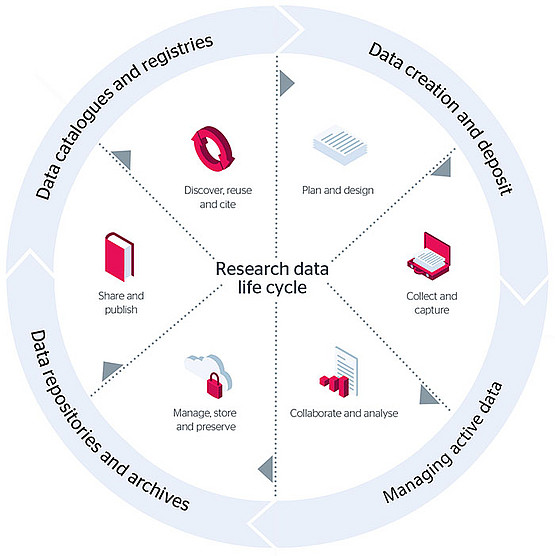
\includegraphics[width=.5\textwidth]{rdm-lifecycle-jisc.png}
	\caption[The life cycle of digital research objects]{The life cycle of digital research objects. License: JISC Research data management toolkit (\href{https://www.jisc.ac.uk/guides/rdm-toolkit}{www.jisc.ac.uk/guides/rdm-toolkit}), CC-BY-ND}
	\label{fig:rdm-lifecycle}
\end{figure}


\subsection{The FAIR guiding principles for scientific data management and stewardship}

Since their publication, the so-called \glsunset{FAIR}\gls{FAIR} principles \citep{wilkinson2016fair} have become guidelines for \gls{rdm} efforts for digital research objects.
They describe four measurable properties of research data that -- the better they are fulfilled -- serve the ultimate goal to improve the discoverability and reusability of data by machines and humans alike \citep{wilkinson2016fair}.
The \gls{FAIR}ness of data can be improved on each of the four related but separable major characteristics that are behind the \gls{FAIR} acronym (taken verbatim from \citet{wilkinson2016fair}):

\begin{itemize}
	\item \textbf{F}indable: To be Findable, (meta)data  are assigned a globally unique and persistent identifier (F1); data are described with rich metadata (F2); metadata clearly and explicitly include the identifier of the data it describes (F3);  (meta)data are registered or indexed in a searchable resource (F4)
	\item \textbf{A}ccessible: To be Accessible, (meta)data are retrievable by their identifier using a standardized communications protocol (A1); the protocol is open, free, and universally implementable (A1.1); the protocol allows for an authentication and authorization procedure, where necessary (A1.2);  metadata are accessible, even when the data are no longer available (A2)
	\item \textbf{I}nteroperable:  To be Interoperable, (meta)data use a formal, accessible, shared, and broadly applicable language for knowledge representation (I1); (meta)data use vocabularies that follow FAIR principles (I2); (meta)data include qualified references to other (meta)data (I3); and
	\item \textbf{R}eusable: To be Reusable, meta(data) are richly described with a plurality of accurate and relevant attributes (R1); (meta)data are released with a clear and accessible data usage license (R1.1); (meta)data are associated with detailed provenance (R1.2); (meta)data meet domain-relevant community standards (R1.3)
\end{itemize}

A pivotal factor for the importance of the FAIR principles is the increasing digitization of research practice, and with it, a rapid growth in research data \citep{dfg}.
Innovation relies on the ability to integrate new and existing data, and where the amount of data to discover, understand, and consolidate requires automation, research objects themselves need to become self-descriptive.
For this, the term ``machine-actionable'' is central to the \gls{FAIR} principles.
It is used to describe an ideal state in which a digital object provides detailed information (metadata) to an autonomously-acting, computational data explorer in two possible contexts: For one, as metadata about the object (``What is it?''), and second, as metadata about its content (``How do I process it?'') \citep{wilkinson2016fair}.
Notably, the \gls{FAIR} principles do not suggest specific metadata standards, implementations, or technology choices.
They do highlight the importance of community-endorsed vocabularies, however, and advocate to either extend them if they do not yet include the attributes required for rich annotations, or create suitable new community-endorsed vocabularies. \\
The end state of FAIR \gls{rdm} for any digital research object is a high quality digital publication that facilitates and simplifies its discovery, evaluation, and reuse in downstream studies.
This reusability refers to the further use or utilization inside or outside its original research context, by the original author or different actors.
It is arguably the most important feature of a research object for various stakeholders: It can make research more efficient, foster collaborations, and speed up progress, and as it can reduce duplicate efforts it constitutes an economical benefit for funders as well as the public and industry \citep{nfdi2022data}.
Considering additional time spent, cost of redundant storage, licensing costs, research retraction, double funding, and missed potential for economic growth, the European Commission estimates that the cost of not having FAIR data lies between 10 and 26 billion euro per year \citep{eu2019FAIR}.
The largest position in their cost-benefit analysis is the time wasted by researchers when non-FAIR data takes more time to find, retrieve, clean, integrate, and peer review.
Together with the aspect of research retraction, the last point hints at an important side effect of good data management: Reproducibility.
Throughout this thesis, the connection between research data management and reproducibility will be exemplified.
The following sections will outline \gls{rdm} requirements and solutions in the field of neuroimaging that work towards this goal.


% Internationally accepted standard
%The largest funding institution for the sciences and humanities and research in Germany, the \gls{grf}, states that access to data and software according the the FAIR principles are of comparable importance to science as access to publications \citep{dfg}





\subsection{Research data management in neuroimaging}
\label{chap:k1-rdm-2}

%\[
%\left[
%\begin{tabular}{@{\quad}m{.3\textwidth}@{\qquad}m{.6\textwidth}@{\quad}}
%	\includegraphics[width=.7\linewidth]{qr_pub_niso.png} &
%	\raggedright%
%	\textbf{Related publications} \par
%	The following section contains a subset of the work presented in our original publication \citet{NISO2022119623}.
	%
%\end{tabular}
%\right]
%\]


Neuroimaging data poses a number of additional challenges for research data management.
For one, the field is characterized by complex datasets.
They typically encompass different modalities (such as imaging, electro-physiological, and behavioral measurements), and often entail several recording sessions.
The \gls{BIDS} \citep{gorgolewski2016brain} is a community-endorsed standard for organizing and describing neuroimaging data, and is widely considered as a successful solution for data standardization in such datasets.
It defines common and modality specific schemes for file names and file organization, file formats, and metadata to accompany raw  or derived data, i.e., both original acquisitions as well as the outputs of common processing pipelines.
\gls{BIDS} has widespread and growing support for different neuroimaging modalities, and is made a common prerequisite by neuroscientific data portals such as OpenNeuro \citep{markiewicz2021openneuro} or processing tools such as BIDSApps \citep{gorgolewski2017bids} or fMRIprep \citep{esteban2019fmriprep}.
An example of an \gls{meg} dataset, structured to \gls{BIDS} or organized idiosyncratically, is shown in \cref{fig:BIDS}. \\
The storage demands of neuroimaging data are not trivial, either.
\gls{BIDS} regulates which file formats must be used for which data type, and focuses on open file formats for accessibility and compression to reduce disk space requirements.
But neuroimaging data are nevertheless sizable \citep{van2014human}.
And a growing awareness that robust findings require sufficiently long recordings \citep{li2021moving} as well as large and representative samples \citep{button2013power, turner2018small} leads to large-scale datasets such as the \gls{HCP} \citep{van2013wu}, the \gls{ABCD} Study \citep{casey2018adolescent}, or the \gls{UKB} project \citep{matthews2015uk} that pose infrastructural challenges for storage, analysis, transfer and archival.
Moreover, in human neuroimaging, data underlie strict data protection regulations such as the \gls{HIPAA} in the United States, or the \gls{GDPR} in Europe.
This requires compliance to variable terms of data usage agreements, and often involves idiosyncratic processes to retrieve data \citep{waitedata}.\\
Processing of neuroimaging data is complex, too.
It usually involves multi-stepped workflows from acquisition through analysis to archival, where each step frequently requires several different software tools \citep{poline2011, NISO2022119623}.
The number of ``researchers' degrees of freedom'' -- the amount of possible combinations of methods, parameters, and tools -- in neuroimaging analyses is thus large \citep{bowring2019exploring}.
But variations in analytic choices affect numeric results and conclusions \citep{silberzahn2018}.
When \citet{botvinik2020variability} instructed 70 independent research teams to analyze the same task-based \gls{fMRI} dataset with tools and methods of their choice to test the same hypotheses, conclusions were highly variable.
A similar project, EEGManyPipelines (\href{https://eegmanypipelines.org/}{eegmanypipelines.org}), is currently ongoing in the field of \gls{eeg}, and expects to find even more variability.
One central aspect \gls{rdm} thus needs to provide in neuroimaging is precise information about how tools, data, and actors were involved in the generation of a file.
This is necessary because, despite reporting guidelines for \gls{MRI} \citep{nichols2017best}, \gls{meg} \citep{pernet2020issues}, and \gls{eeg} \citep{styles2021towards} studies, traditional publications still regularly fail to report all relevant details about recording, processing, and analysis  \citep[see, e.g.,][]{vsovskic2022better}.
Such \textit{digital provenance} (illustrated in \cref{fig:prov1}) is not meant to decrease the analytical variability.
Instead, it captures thorough, machine-actionable processing descriptions that are necessary to investigate differences between analysis outcomes, reproduce, or reuse them as \gls{FAIR} principle R2 advocates.
Chapter \ref{chap:k3} will further elaborate on this problem.\\
Overall, careful \gls{rdm} is necessary to translate complex data with difficult storage requirements and sophisticated processing workflows efficiently into scientific insights in the field of neuroimaging.
Given these specific complexities, solutions to these challenges often arise from the community of researchers.
The following section will highlight one of several software tools that aids with the complex task of research data management: DataLad.
%A subsequent chapter, \cref{chap:k2}, will later focus on how research data management is a prerequisite of reproducible research, specifically with regards to software environments and large sample sizes.
%In addition, \cref{chap:k2} will highlight pragmatic approaches to \gls{rdm} that can be embedded in standard research practice and contribute to the FAIRification of data, even in absence of established metadata formats.

%BIDS
\begin{figure}
	{\scriptsize
		\begin{minipage}{.49\textwidth}
			\begin{forest}
				pic dir tree,
				for tree={% kleiner Zeilenabstand
					s sep=0.02cm}
				[memento/
				[memento\_001/
				%		[Move\_correc\_SSS\_alignedinitial\_nonfitiso/
				%		[1\_memento\_001\_ml83-1\_mc\_transforminitial.fif, file]
				%		[2\_memento\_001\_ml83-1\_mc\_transforminitial.fif, file]
				%		[3\_memento\_001\_ml83-2\_mc\_transforminitial.fif, file]
				%		[data\_fix1.mat, file]
				%		[data\_fix\_ft1.mat, file]
				%		[data\_fix\_new1.mat, file]
				%		[data\_fix\_reduced1.mat, file]
				%		[delay\_photodiode\_subject\_long\_default\_realign\_only\_ICA1.mat, file]
				%		[memento\_results\_ICA\_newall\_alignedinitial228.mat, file]
				%		[memento\_results\_ICA\_newall\_alignedinitial461.mat, file]
				%		[memento\_results\_ICA\_newall\_alignedinitial511.mat, file]
				%		[num\_trials\_old\_ICA.mat, file]
				%		[resultfile\_probs-1.mat, file]
				%		[trial\_out\_ind.mat, file]
				%		]
				[Move\_correc\_SSS\_realigneddefault\_nonfittoiso/
				[1\_memento\_001\_ml83\_mc\_realigneddefault.fif, file]
				[2\_memento\_001\_ml83-1\_mc\_realigned\_default.fif, file]
				[3\_memento\_001\_ml83-1\_mc\_realigned\_default.fif, file]
				[memento\_results\_ICA228.mat, file]
				[memento\_results\_ICA455.mat, file]
				[memento\_results\_ICA461.mat, file]
				[memento\_results\_ICA511.mat, file]
				[memento\_results\_ICA\_newall228.mat, file]
				[memento\_results\_ICA\_newall455.mat, file]
				[memento\_results\_ICA\_newall461.mat, file]
				[memento\_results\_ICA\_newall511.mat, file]
				[mri\_aligned.mat, file]
				[num\_trials\_old\_ICA.mat, file]
				[outfile\_new\_all.mat, file]
				[resultfile\_new\_all.mat, file]
				[template\_grid.mat, file]
				[trial\_out\_ind.mat, file]
				]
				[Raw/
				[1\_memento\_001\_ml83.fif, file]
				[2\_memento\_001\_ml83-1.fif, file]
				[memento\_001\_ml83-2.fif, file]
				]
				]
				]
			\end{forest}
		\end{minipage}
		\quad
		\begin{minipage}{.49\textwidth}
			\begin{forest}
				pic dir tree,
				for tree={% kleiner Zeilenabstand
					s sep=0.02cm}
				[memento/
				[dataset\_description.json, file]
				[participants.json, file]
				[participants.tsv, file]
				[README, file]
				[sub-001/
				[meg/
				[sub-001\_acq-calibration\_meg.dat, file]
				[sub-001\_acq-crosstalk\_meg.fif, file]
				[sub-001\_coordsystem.json, file]
				[sub-001\_task-memento\_channels.tsv, file]
				[sub-001\_task-memento\_events.tsv, file]
				[sub-001\_task-memento\_log.tsv, file]
				[sub-001\_task-memento\_meg.json, file]
				[sub-001\_task-memento\_split-01\_meg.fif, file]
				[sub-001\_task-memento\_split-02\_meg.fif, file]
				[sub-001\_task-memento\_split-03\_meg.fif, file]
				]
				[sub-001\_scans.tsv, file]
				]
				]
			\end{forest}
		\end{minipage}
	}
	\caption[An example of a BIDS-structured dataset]{A real-world example of a single subject's MEG acquisition. The left side shows the file tree of the data from a project directory with an idiosyncratic organization. It includes a mix of raw data, preprocessed data, and intermediate results, and the naming scheme is inconsistent. The right side shows the same subject's data, but structured according to \gls{BIDS}. The naming scheme is consistent, and apart from raw MEG data the directory includes metadata files from the experiment and acquisition machine that are required to understand the data without the original authors.}
	\label{fig:BIDS}
\end{figure}


% provenance
\begin{figure}
	\centering
	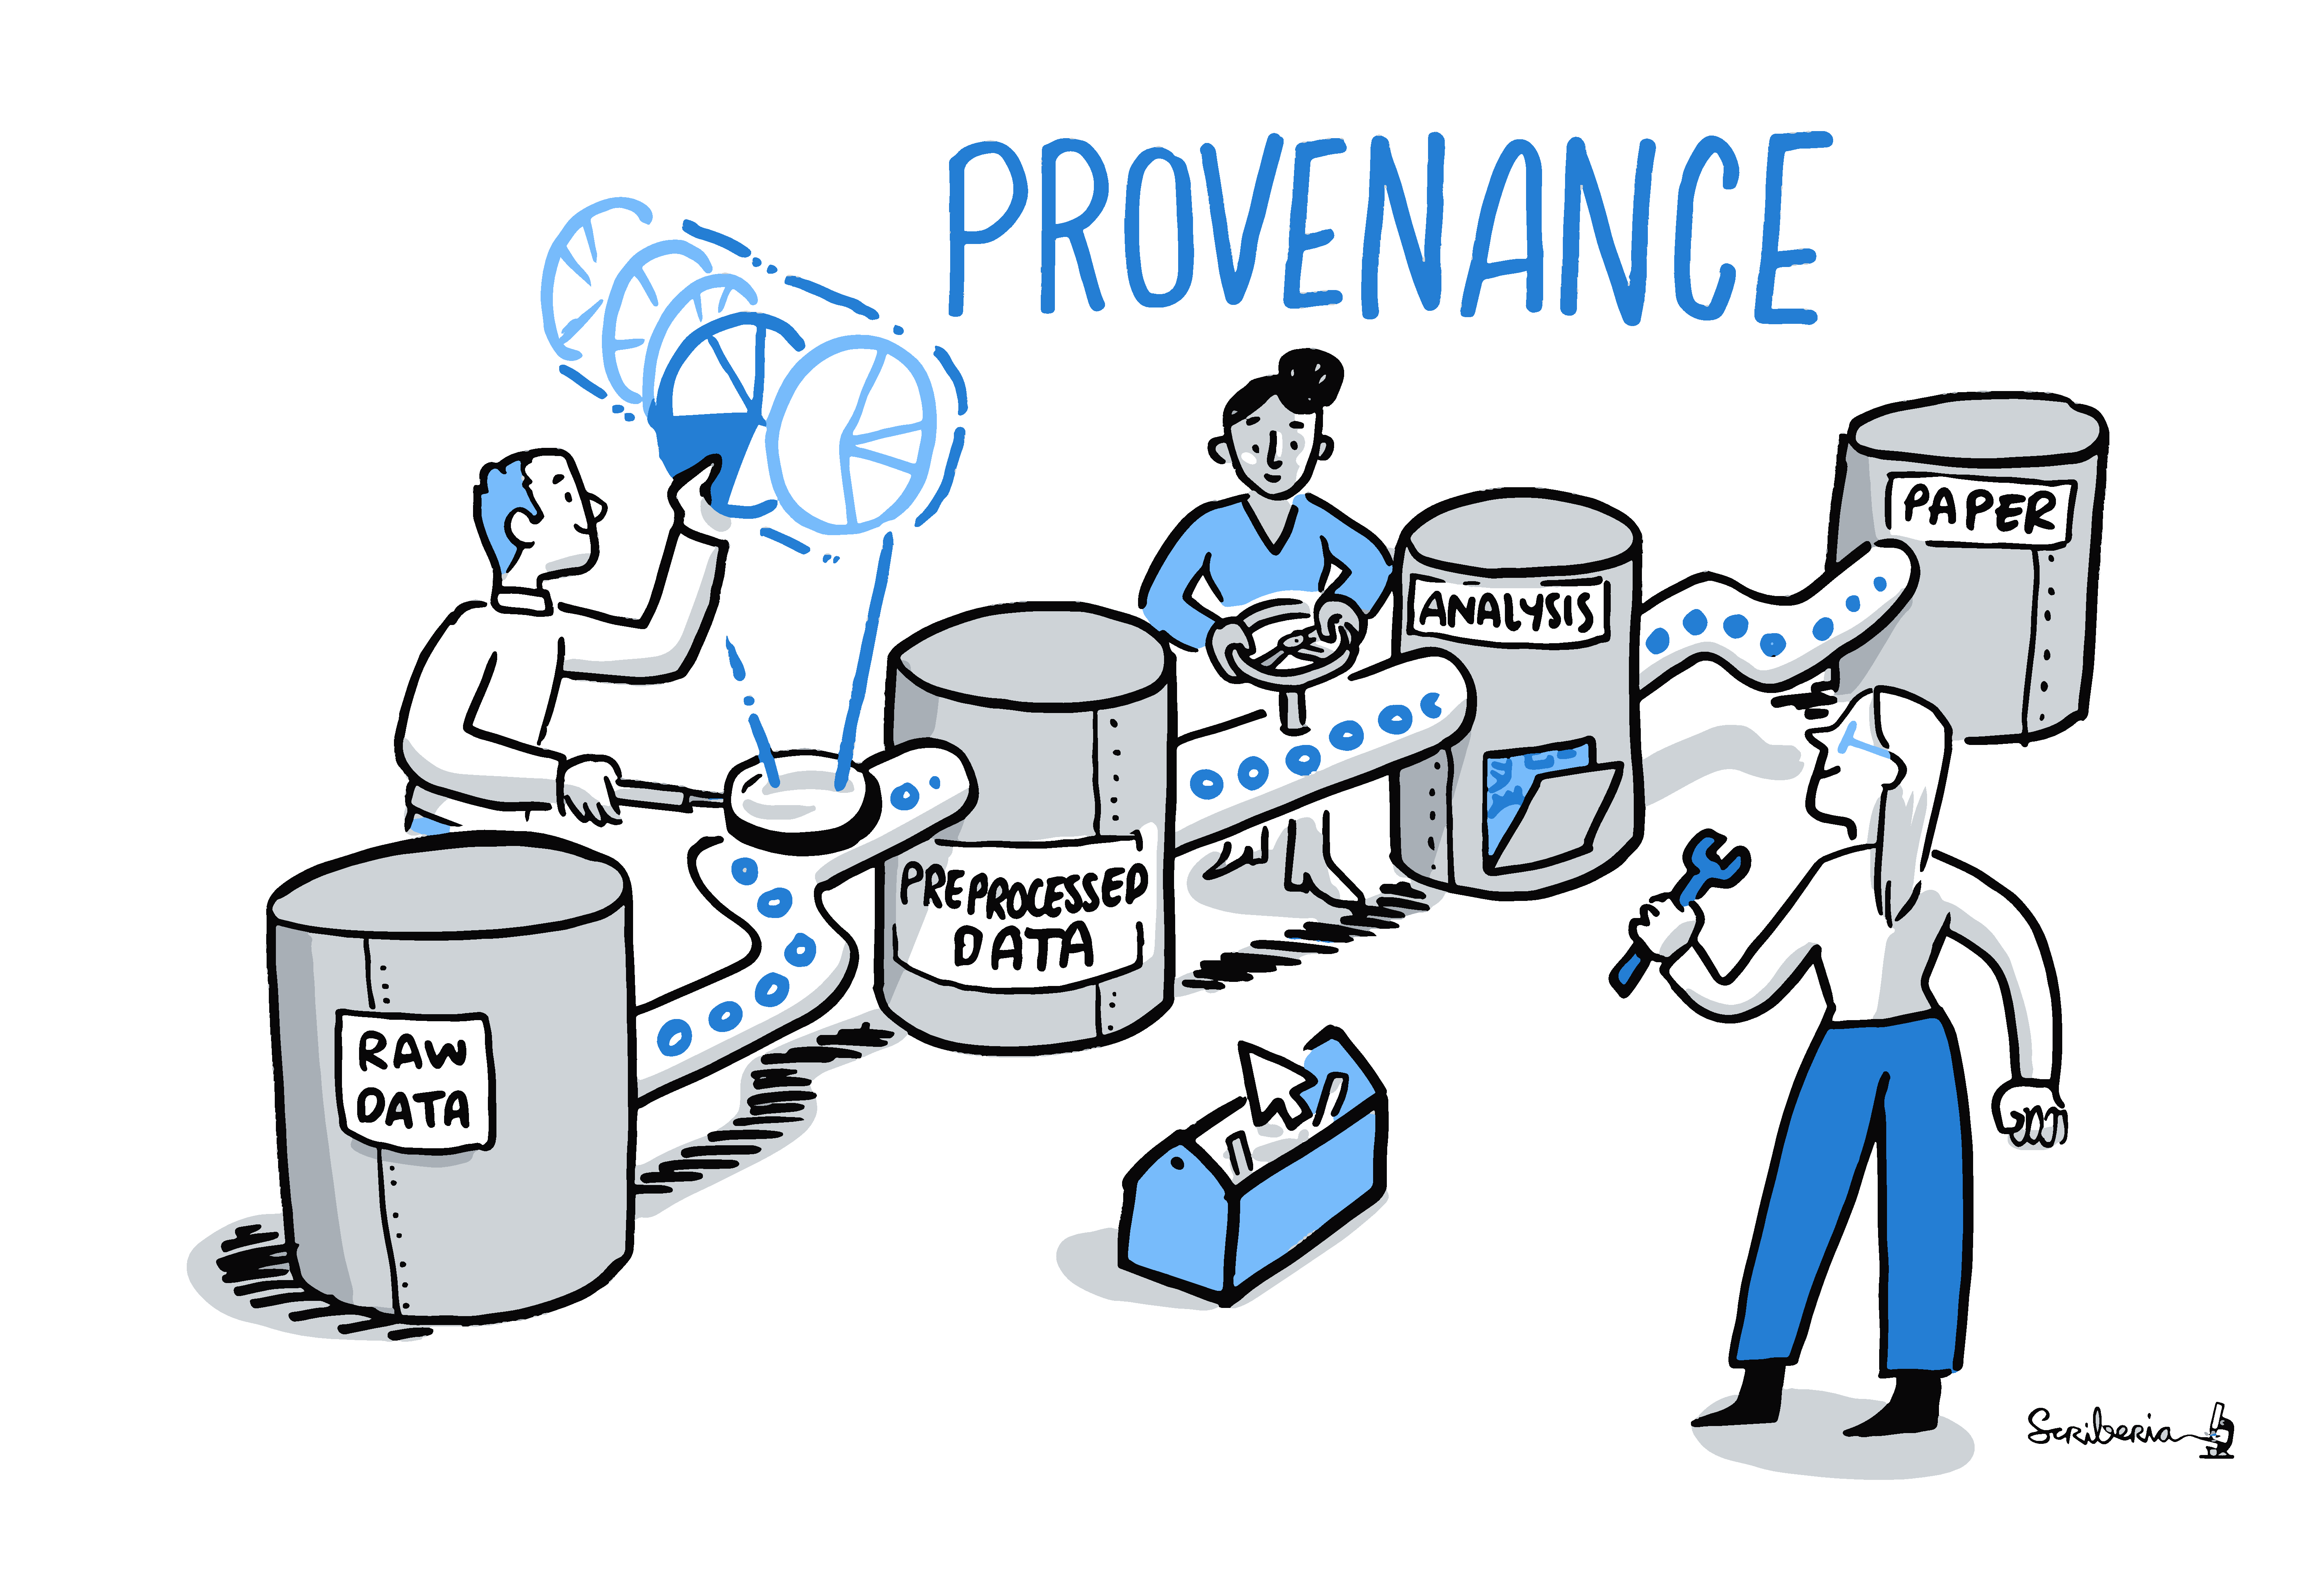
\includegraphics[width=.5\textwidth]{provenance.pdf}
	\caption[Provenance throughout the research process]{In multi-stepped analyses, a variety of choices affect the final outcome. Digital provenance, information about how tools, data, and actors were involved in the generation of file, is required to retrace, understand, and trust the decisions that led to a research outcome. Such provenance can be an outcome of good research data management. License: Scriberia and the Turing Way Project, CC-BY}
	\label{fig:prov1}
\end{figure}



% link to chapter 3: Research data management is a prerequisite of reproducible research

\section{DataLad as a software solution for research data management challenges}

%\[
%\left[
%\begin{tabular}{@{\quad}m{.3\textwidth}@{\qquad}m{.6\textwidth}@{\quad}}
%	\includegraphics[width=.7\linewidth]{qr_pub_datalad.png} &
%	\raggedright%
%	\textbf{Related publications} \par
	The following section provides an overview of the software tool DataLad and its use for research data management.
	The reader is invited to refer to our original publication \citep{Halchenko2021} for a more detailed description.%
%\end{tabular}
%\right]
%\]

%This introduces DataLad as a software solution for research data management

DataLad (\href{http://datalad.org}{datalad.org}) is a Python-based, MIT-licensed software tool for the joint management of code, data, and their relationship.
It builds up on git-annex, a versatile system for data logistics \citep{hessannex}, and Git, the industry standard for distributed version control.
To address the technical challenges of data management, data sharing, and digital provenance collection, it adapts principles of open-source software development and distribution to scientific workflows. \\
%Initially, DataLad development started with the idea to make data retrieval as easy as installing software with package managers on Unix-based operating systems\footnote{On a Debian system, a user can install thousands of software package with a single command such as \texttt{apt get install <package-name>}.}.
%Now, DataLad aims to make data management as easy as managing code \citep{Halchenko2021}.
DataLad's aim is ``to make data management as easy as managing code'' \citep{Halchenko2021}.
The latter benefits from a well-established ecosystem of tools, platforms, and processes.
The distributed version control tool Git provides the ability to track changes in small-sized, text-based files, and is a de-facto standard in collaborative software development. In 2022, 93.78\% of respondents in Stackoverflow's annual developer survey (\url{survey.stackoverflow.co}) reported to use it.
Hosting platforms for Git repositories such as GitHub (\url{github.com}), GitLab ({\url{gitlab.com}), or Gin (\url{gin.g-node.org}) have been developed to serve as facilitators for collaboration, discovery, and reuse.
In the scientific community it is widely recommended to employ version control for code to foster reproducibility \citep[e.g.,][]{sandve2013ten}, and it is established practice to develop and share research software and code using Git and Git hosting platforms \citep[e.g.,][]{nord2019towards, strupler2017reproducibility, bryan2018excuse, corti2019managing}.
But other components of scientific projects, such as data or computing environments, are not as transparently managed or accessible as code and software.
Digital research objects are usually stored in multiple different locations \citep{parsons2013research}, and their consumption is complicated by disconnected and non-interoperable hosting solutions:
Different storage services use different protocols, means of authentication, or other idiosyncrasies that require custom workflows.
Moreover, as will be elaborated in chapter \ref{chap:k3}, scientific computation is not reproducible enough, because data provenance is often incomplete and rarely automatically captured.
And over the course of a research project, often as part of the standard, multi-stepped processing workflow, data evolve and change just like code does:
Continued acquisitions enlarge the raw dataset; Transformations to -- likewise evolving -- community standards change file formats, dataset organization, or enrich available metadata; And continuous quality control processes can fix errors in datasets.
In the case that data or other research objects were subject to change over the course of a project, there is a need to identify which exact version has been used -- otherwise, the reproducibility of a result is threatened \citep{hardwicke2018data}.
Yet unlike code in software development, data tend not to be as precisely identifiable because data versioning is rarely or only coarsely practiced.
Last but not least, in the absence of standardized data packages, there is no uniform way to declare actionable
data dependencies and derivative relationships between inputs and outputs of a computation.
Consequentially, data needs to be kept alongside to results to ensure reproducibility, even if it is hosted elsewhere already.
Especially in the age of big data neuroscience \citep{bzdok2017inference}, downloads or storage of datasets can become infeasible \citep{horien2021hitchhiker, grisham2016proposed}.
And although projects might only draw insights from only a subset of a dataset, such as only specific modalities, tasks, or participants, a project has heavier disk space demands if the original dataset is only available as a bulk download.\\
DataLad aims to solve these issues by providing streamlined, transparent management of code, data, computing environments, and their relationship.
Its main features are 1) Version control for data of any size or type; 2) Streamlined procedures to consume, publish, and update  all elements of scientific projects, with interoperability adapters to established scientific and commercial tools and services; 3) Data linkage as precisely versioned, lightweight dependencies; And 4) actionable process provenance capture for arbitrary command execution that affords automatic re-execution.

\subsection{Technical features}

Fundamental to DataLad's functionality is the concept of the ``DataLad dataset'', DataLad's central data structure.
On a technical level, it is a joint Git and git-annex repository with additional metadata and features for scientific use cases added on top by DataLad.\\
Git excels at managing and collaborating on text files, and provides a powerful back bone to DataLad's features.
Git repositories can be easily distributed as linked \textit{clones} to suitable infrastructure to share files and their revision history.
Locally, changes to files can be saved (\textit{committed}) with detailed provenance and transferred (\textit{pushed}) to all clones of a repository, and remote revisions can be retrieved and integrated (\textit{pulled}).\\
However, Git is not designed to handle large or binary files as common in science.
Git-annex overcomes this limitation and adds support to track and transfer files of arbitrary size or type without placing their content into Git.
Instead, it places file content into a managed repository \textit{annex} and only commits a lightweight reference that encodes the file's name and content identity via content hash into Git.
This reference allows a decoupling of file content (handled by git-annex) and file name (tracked with Git), but retains the ability to transparently notice and track changes: If file content changes, the identity reference known to Git changes, too, and the version control system becomes aware of the modification.
The same mechanism guarantees file integrity at all times and solves data privacy concerns without impacting discoverability, as potentially sensitive content can be kept private but its metadata can be distributed easily.
While Git keeps a reference of the content \textit{identity}, git-annex tracks content \textit{availability}, and manages data transport with an extensible set of protocols and set of hosting solutions to and from a local repository annex at a granularity of individual files. \\
DataLad, finally, extends Git and git-annex with easy to use modularization, re-executable annotation of changes, and targeted interfaces and interoperability adapters.\\
Modularization facilitates reusability in research workflows.
Scientific projects can encompass a large amount of files, or have a heterogeneous nature, comprising different data sources or evolving data across different processing stages.
Organizing them into a modular structure of homogeneous or smaller components enables more efficient reuse.
DataLad allows to nest individual datasets via versioned linkage as lightweight dependencies, and provides seamless recursive operations across dataset boundaries by extending Git’s submodule mechanism.
With this, DataLad provides a ``monorepo''-like user experience in datasets with arbitrarily deep nesting, and makes it trivial to operate on individual files deep in the hierarchy or entire trees of datasets, while individual datasets can easily be reused in new contexts (see \cref{fig:subdslinkage}).\\
Re-executable annotations of changes constitute process provenance.
In DataLad datasets, DataLad can wrap any command execution and automatically capture the command, the generated outputs or modification, and optionally all required input elements with a so-called \texttt{datalad run} or a \texttt{datalad containers-run} command.
The former command captures the execution of any shell command, and the latter command can use software containers, tracked in DataLad datasets, for executing commands inside a specific software environment or containerized pipeline.
Both commands retrieve inputs, initiate command execution, and, if it succeeds, save results together with a re-executable provenance in a structured annotation to a Git commit message (see)\cref{fig:fairly_metadata}).
In addition to providing reliable information about past command-line invocations, these machine-readable records make it possible to easily re-execute commands, for example to verify if a result is computationally reproducible or to apply an analog change to a different dataset state.\\
Interoperability adapters, finally, streamline data publication and consumption routines.
Being able to efficiently retrieve and update research objects across a variety of available storage options is an important part of \gls{rdm} \citep{borghi2018data}.
Git can already interact with other local or remote repositories via standard or custom network transport protocols, and git-annex readily provides access to a wide range of external data storage resources via a large set of protocols.
On top of this, DataLad implements support for additional services that require custom protocols, such as the \gls{osf} \citep{hanke2021dlosf} or XNAT \citep[\url{www.xnat.org},][]{halchenko2021xnat}, and can add more fine-grained access (e.g. direct access to individual components contained in an archive hosted on cloud storage).
With this approach, DataLad can help to overcome technological limitations of storage solutions, or integrate seamlessly with technology that is already in use.

\begin{figure}
	\centering
	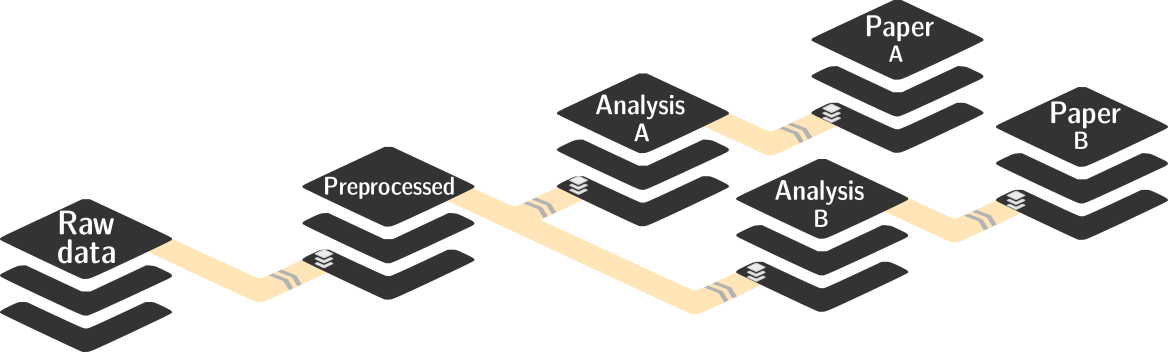
\includegraphics[width=.6\textwidth]{linkage_subds.png}
	\caption[DataLad dataset linkage]{Exemplary dataset hierarchy in a research project. DataLad datasets can be linked as actionable superdataset-subdataset relationsships. This allows, for example, to add a DataLad dataset with preprocessed data in a dependency-like link to an analysis. As DataLad datasets decouple sizable file content from file availability metadata, such links are only a fraction of the size of the data they track. At the same time, linkage is seamless, and DataLad operations can work across dataset boundaries. This feature enables modular projects from stand-alone units that facilitate reuse.}
	\label{fig:subdslinkage}
\end{figure}

\subsection{Development principles}

DataLad's development is guided by four principles \citep{Halchenko2021}:
\begin{itemize}
	\item The only two recognized entities are Datasets and the files they comprise,
	\item A dataset is a Git repository with an optional annex,
	\item The should be as few custom procedures and data structures as possible,
	\item Complete decentralization, with no required central server or service, but maximum interoperability with existing 3rd-party resources and infrastructure.
\end{itemize}

These principles ensure DataLad's open and domain agnostic nature, maximize the long-term utility of DataLad datasets, minimize users' technical debt and reduce the risk of adoption.
When using DataLad datasets for digital objects, access to any resource managed with DataLad has no critical dependency on service deployments governed by central entities, and even on DataLad itself.
A further characteristic is that DataLad is developed not as a singular tool, but as an extensible ecosystem of software packages.
A core package provides basic functionality, and DataLad extensions, stand-alone Python packages with additional DataLad functionality, can enhance it with domain-focused or technology-specific features.
This aims to keep the source code maintainable, and allows users to tune the command-suite to their specific needs.


\subsection{User experience}

On the conceptual level, a DataLad dataset is an overlay structure to version control files of any size, track and publish files in a distributed fashion, and record, publish, and execute actionable provenance of files and file
transformations.
On a file system, it appears like a regular directory.
Users can either create DataLad datasets from scratch (\texttt{datalad create}) or install them from a variety of sources (\texttt{datalad clone}).
When consuming DataLad datasets from external sources, annexed file content can be retrieved (\texttt{datalad get}) and removed (\texttt{datalad drop}) on demand if the given user has potentially necessary access rights.
Generally, DataLad's commands aim to simplify standard workflows from Git, git-annex, or hosting services to make them more accessible to technical novices.
For example, committing a file into Git requires a \texttt{git add} followed by a \texttt{git commit}, and annexing a file requires a \texttt{git annex add} followed by a \texttt{git commit}.
A \texttt{datalad save}, on the other hand, performs either action, with automatic decision making whether the file is annexed or committed to Git.
Likewise, publishing a repository to hosting sites usually requires interactions in the hosting site's web interface, but DataLad provides a set of \texttt{create-sibling-<service>} commands that spare users the need to visit the hosting service.
And publication dependencies or automatic configurations can publish Git revision history and annexed file contents conjunctly, using \texttt{datalad push}.
Provenance capture can be achieved by wrapping command executions in either a \texttt{datalad run} or \texttt{datalad containers-run}\footnote{The \texttt{datalad containers-run} command is provided by the \texttt{datalad-container} extension package, available with standard Python package managers.} command, and they can be re-executed using \texttt{datalad rerun} (see \cref{fig:fairly_metadata}).
When working in hierarchies of datasets, any command's \texttt{--recursive} parameter applies it to downstream datasets.
Despite the fact that DataLad provides its own set of commands, compatibility with all Git and git-annex functionality is retained, and users are free to chose their workflows.
Like Git and git-annex, DataLad is primarily developed as a command line tool, but a \gls{gui} exists as well (see \cref{fig:gooey}).\\
With DataLad's streamlined data transport routines, users cab utilize web sources, including major cloud storage providers, paths on local or remote computational infrastructure, or neuroscientific data registries such as OpenNeuro \citep{markiewicz2021openneuro} for file storage or collaboration.
At the same time, the separation of file content and file name makes a lean, meta-data based representation independent from actual data retrieval.
Thus, datasets of arbitrary scale can be cloned, exposing file names and revision history of all contained files, and provide actionable access to its content at a fraction of their total size.
And in order to expose datasets for easier access, users can publish DataLad datasets to common repository hosting infrastructure as access points to install data, without actually publishing data contents to these services.
These features aid with \gls{rdm} tasks in scientific projects.
A thorough overview of them can be found in the software's documentation, which is elaborated on in chapter \ref{chap:k2}, and a comprehensive use case is detailed in chapter \ref{chap:k3}.

% provenance
\begin{figure}
	\centering
	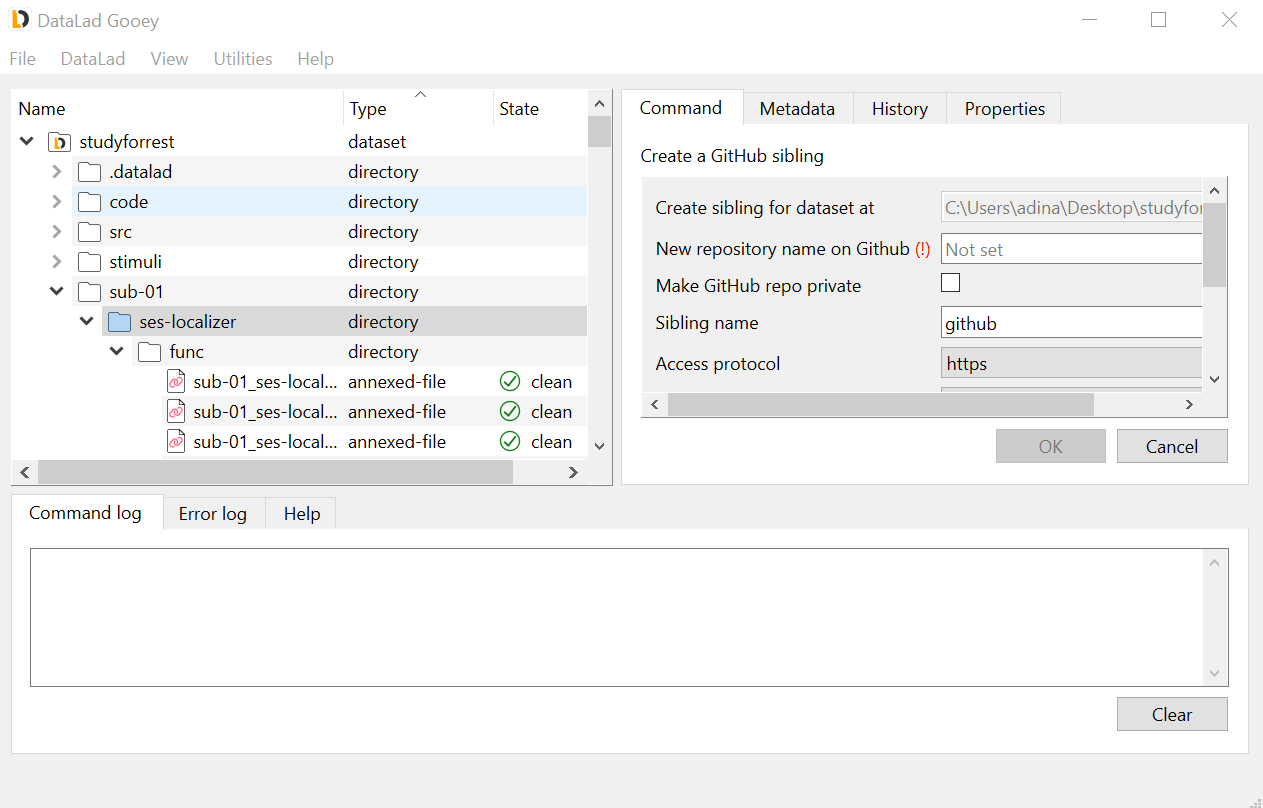
\includegraphics[width=.9\textwidth]{datalad_gooey.png}
	\caption[DataLad: Graphical User Interface]{The \gls{gui} of DataLad on a Windows system, provided by an extension package \texttt{datalad-gooey}. A file tree (left) provides an overview of the file system, and annotates elements into DataLad datasets, contents tracked with Git or git-annex, untracked, modified, or clean states. A command window (right) as well as right-click drop down menus (not shown) lets users parametrize and execute DataLad commands. A log window (bottom) can display result outcomes, error, or help text.}
	\label{fig:gooey}
\end{figure}



\subsection{Software adoption and relevance}

As DataLad does not employ tracking code, the exact number of its users is not known.
However, download statistics from the major Python package managers \texttt{pip} and \texttt{conda}, and popularity statistics from users of the Debian operating system can provide rough references.
According to \url{pypistats.org}, the main DataLad Python package was downloaded from the Python Package Index 300 times per day on average in May 2023.
The Python distribution Anaconda (\url{anaconda.org}) counts a total of 333932 downloads of the software throughout versions 0.9.3 (April 2018) and 0.18.3 (May 2023), averaging 180 downloads per day.
The \texttt{popularity-contest} software is a Debian package that, if installed on a users system, reports anonymous statistics about most-used Debian packages.
This data is aggregated into a popularity contest.
According to it, in May 2023 between 0.08 and 0.1 percent of systems reporting statistics have a DataLad installation (see \cref{fig:popcon}).
All of these sources contain biases that limit conclusion to the number of users, though.
Installations via Python package managers are commonly performed by individual end users, whereas installations of Debian packages can correspond to system-wide installations on multi-user systems such as high performance computing infrastructure.
Likewise, upgrades of existing installations to more recent versions are included in these data, as well as temporary installations of the software in automated continuous integration test suites.
Nevertheless, download statistics attest that it is an actively used tool with a user base that exceeds the circle of its developers by far.
The citation count of the academic paper, totaling 53 in May 2023, 1.5 years after its publication by \citet{Halchenko2021}, and active contributor community around the source repository on GitHub, currently amounting to 48 individuals with committed code contributions, confirms that.
DataLad's current popularity, however, has not been established from the beginning of its development.
The next chapter will highlight how scientific software like DataLad can be improved and gain popularity, and, vice versa improve scientific practice.



% !TeX root = ../main-english.tex
% !TeX spellcheck = en-US
% !TeX encoding = utf8
% -*- coding:utf-8 mod:LaTeX -*-

%This smart spell only works if no changes have been made to the chapter
%using the options proposed in preambel/chapterheads.tex.
\setchapterpreamble[u]{%
	\dictum[Carole Goble]{Better Software, Better Research}
}

%\chapter{Improving scientific practice through software usability: The DataLad Handbook}
\chapter{Improving scientific practice through software usability}
\label{chap:k2}



Scientific software is an integral part of the research process, and improving the quality of research software benefits the research itfelf \citep{goble2014better}.
This next chapter details how a documentation project for DataLad increased software quality, software popularity and enabled users to tackle complex \gls{rdm} use cases.
It refers to our original publication \citep{wagner2020datalad}.


\section{The central role of research software in science}

% Whats scientific software?

Scientific software, often also referred to as research software, can broadly be defined as software used for scientific purposes.
As software requirements for scientific use cases can be specialized, the developers of research software often overlap with the community of scientists that uses the software \citep{hannay2009scientists}, and over the past decade, the term ``Research Software Engineer'' has been established to describe researchers that dedicate parts of their scientific work to creating and maintaining software \citep{hettrickRSE}.

% Why is it important?
Scientific software is an integral part of research in science, engineering, and humanities.
The majority of scientific work could not be done without software, thus, fittingly, the United Kingdom's Engineering and Physical Sciences Research Council describes it as a ``critical infrastructure that underpins cutting edge science and engineering research'' (CITATION) % https://www.ukri.org/what-we-offer/browse-our-areas-of-investment-and-support/research-infrastructure-theme/

% recognition
More recently, research software has been gaining academic credit it has long lacked.
It is recognized as academic output in the San Francisco Declaration on Research Assessment (DORA; \href{https://sfdora.org/}{sfdora.org}), and the Agreement on Reforming Research Assessment (CoARA; \href{https://coara.eu}{coara.eu}), both of which have been signed by thousands of academic institutions worldwide. The \gls{grf}, the largest funding institution for the sciences and humanities and research in Germany, counts software a ``scientific result'' in their evaluation of academic CVs.
Academic journals, such as the Journal of Open Source Software (\href{https://joss.theoj.org/}{joss.theoj.org}), and article types, such as Nature's ``Toolbox'' (\href{https://www.nature.com/nature/articles?type=toolbox}{www.nature.com/nature/articles?type=toolbox}), have been created to support the scholarly publication and reuse of research software.

% the need to improve
With the acknowledgment of the importance of scientific software in research, there also is an awareness that its quality, reusability, and longevity needs to be ensured and improved.

One of the strategies for this is to make research software open source.
% why does open source improve
For example, Open Source is recommended by the \gls{grf} \citep{dfg}.

And calls for proposals to improve the quality, usability or longevity of research software have been put forward by major national funders, including Germany \citep{dfgrs}, the United Kingdom \citep{ukri}, and the United States \citep{nih}.

One set of problems from which software quality can suffer are documentation deficiencies (CITATION NEEDED).
The mere existence of software is insufficient to ensure its uptake and use according to best practices.
To improve scientific practice, research software needs to enable and empower their users through usability and documentation.
This makes documentation a major factor in the success of scientific software, and an integral part of the software development process.\\
The next section will explore this problem and its consequences.


\subsection{Documentation deficits of scientific software and their consequences}


% what is documentation, provide definitions/delineations
Documentation is information about a software.
It fulfills different roles depending on its target audience, and the literature distinguishes several different types of documentation.
\citet{Parnas2011} categorizes documentation either as a \textit{tutorial} or as a \textit{reference work}.
Both kinds are needed for different audiences: Whereas experienced users and contributors need reference documents to guide further development, such as the elements of an \gls{api}, new users and contributors need a basic understanding of the software tool and its intended use cases.
Commonly distinguished are also \textit{technical} and \textit{user} documentation: The former contains information for developers and users by describing features, maintenance information, or design choices.
The latter targets end users of a software product with accessible explanations how to install a tool, use its features, or step-by-step instructions (CITATION NEEDED). % https://medium.com/@kesiparker/technical-documentation-vs-user-documentation-ff68e7de1985
User documentation also matches the concept of \textit{task-based} documentation, which is broken down into the activities that users will go through as they work, starting with basic tasks and continuing with more advanced tasks that become possible as users continue to work. (CITATION NEEDED) %https://www.linux-magazine.com/Online/Blogs/Off-the-Beat-Bruce-Byfield-s-Blog/Why-projects-need-task-based-documentation

% maybe Design/Architectural docs


% consequences
Research software often lacks comprehensive documentation \citep{segal2007some} \citep{pawlik2012documentation}.
Commonly reported reasons for this are a lack of funding, incentives, and interest by software developers \citep{pawlik2012documentation}.
Yet although it is commonly regarded as separate from the actual piece of software, software documentation is heavily tied to the quality of a software tool and the software development process.
A lack of documentation hinders knowledge transfer both among users and developers, impedes maintenance, and creates a steep learning curve for new users and new developers alike \citep{theunissen}.
\citet{Parnas2011} describes a vicious circle that sets in when the quality of software documentation is poor:
``Reduced [documentation] quality leads to reduced [software] usage, [r]educed [software] usage leads to reductions in both resources and motivation, [r]educed resources and motivation degrade [software] quality further''.
% maybe workflows that break, workflow testing


\section{Documentation in the DataLad project}

Since the first release (0.0.1, March 2015), DataLad had technical documentation with a design overview and a reference documentation.
Any amount of documentation is better than no documentation at all.
However, documentation can still be insufficient if it does not meet the needs of the target audience.
Solely technical or reference documentation, for example, can be suboptimal for novices: It may be incomplete, narrowly focused on individual commands, or assume existing knowledge readers lack (Segal, 2007; Pawlik et al., 2015), and can thereby discourage potential users or inhibit the adoption of a tool.\\
Even though technical documentation is useful for developers, a central target audience for documentation of the DataLad ecosystem are scientists.
While experts in their respective domains and methodologies, scientists may not have domain-agnostic technical skills.
Task sets such as those required in \gls{rdm} require a broad set of technical skills \citep{grisham2016proposed}, and research curricula seldom teach computing ecosystem literacy.
In fact, even computer science curricula often miss critical topics about the computing ecosystem.
At the \gls{MIT}, this lack famously resulted in the internationally popular, self-organized class ``The missing semester of your CS education'' (\href{https://missing.csail.mit.edu/about/}{missing.csail.mit.edu}).
In addition, the high usability of modern computers' and applications' front ends spares users the need to develop the same level of familiarity with their computers than previous generations of computer users had \citep{mehlenbacher2003documentation}.
A considerable part of this target audience can thus be considered technical novices for which technical documentation is not ideal. \\
Research suggests, too, that scientists' needs for documentation go beyond reference manuals.
In an analysis of user questions in support forums of scientific software packages, \citet{swarts2019open} found that the focus in 80\% of inquiries was on operations and tasks, such as a required sequence of operations to achieve a specific goal.
In breaking down user questions by purpose, \citet{swarts2019open} further found that users were most interested in a description of operations or tasks, followed by insights about the reasons behind the action.
And in separating documentation types into ``feature-based'' (closer related to the concept of reference documentation) or ``task-based'',  \citet{swarts2019open} reports twice as many questions seeking explanations in software with feature-based compared to task-based documentation.
This hints at a disconnect between knowing \textit{how} something should be done and \textit{why} it should be done this way.
Overall, it highlights that users of scientific software show a clear need beyond the documentation of individual commands, but seek to understand general usage principles and master complex combinations of features to achieve specified goals.
This type of empowerment is what the DataLad handbook project aimed to achieve.

% Only rarely does a consumer tool involve a terminal instead of a \gls{gui}, and typical applications perform a complete suite of tasks such that users do not need to combine several tools to accomplish one goal (CITATION NEEDED).
% However, powerful scientific tools are often command-line-based (e.g., EXAMPLES), and complex task sets such as those required in \gls{rdm} require a broad set of technical skills \citep{grisham2016proposed}.
% DataLad, too, is primarily developed as a command line tool.

%\pagebreak

\subsection{The DataLad Handbook: A user-focused and workflow-based addition to standard software documentation}

The initial idea to the DataLad Handbook (\href{http://handbook.datalad.org}{handbook.datalad.org}) arose at the 2019 Meeting of the \gls{ohbm}, during the Symposium ``From Open Science to Science: Shifting the status quo in data sharing, software, and publishing''.
Gregory Kiar's presentation ``Technology and Platforms Enabling Reproducible and Open Publishing'' included a recommendation and warning about DataLad: While it would be a powerful tool capable of solving many challenges, users will face difficulties learning which features existed and how they could use them \citep{kiar}.
Motivated by this expressed need of the scientific community for additional guidance, the DataLad Handbook project was initiated.

\subsubsection{Design considerations}
We identified three types of stakeholders with different needs: \textit{Researchers} need accessible educational content to understand and use the tool, \textit{planners}, such as PIs or funders, need high-level, non-technical information in order to make informed yet efficient decisions on whether the tool fulfills their needs, and \textit{trainers} need reliable, open teaching material.
Drawing from personal user experiences with the software, usability research (CITATION NEEDED), and educational concepts (CITATION NEEDED), the Handbook project was set out with the following goals about its contents:

\begin{itemize}
	\item Applicability -> tutorial,  real-world \gls{rdm} applications -> domain-agnostic
	\item Integrative concept of the entire software -> The contents covered by the Handbook need to increase in difficulty, and build up on previous content
	\item Up-to-dateness: tested , up-to-date code snippets
	\item Nevertheless, users should be able to mix-and-match/not have to read the entire documentation
	\item The language should be accessible for technical novices
	\item Trial and error: Common errors are explicitly demonstrated in the safe-space of a tutorial

\end{itemize}

Arising from this specification analysis, the following initial structure was designed to meet the above requirements and fulfill the needs of the three stakeholders \citep{wagner_adina_s_2020_7906718}\footnote{This structure was extended prior to the second release with an additional part ``Beyond Basics'', covering advanced features}:

\begin{itemize}
	\item Introduction: The first part of the book, covering high-level descriptions of the software and its features and detailed installation instructions for all operating systems.
	\item Basics: The second part of the book, written in the form of a continuous, code-along tutorial, set in a domain-agnostic fictional storyline about an \gls{rdm} application
	\item Usecases: The third part of the book, containing short, standalone start-to-end descriptions of real-world usecases, with concise step-by-step instructions, and references to further reading in the Basics.
\end{itemize}

In addition to design and content requirements, the following technical goals were set:

\begin{itemize}
	\item integration test suite
	\item Optional advanced information: Toggleable or custom sections contain extra information. This keeps the visible information consise, but allows for exploration of advanced contents
	\item web-based and printable/downloadable
	\item versioning
\end{itemize}



\subsubsection{The technical backbone}

The technical backbone of the Handbook was chosen with the intent to support declared goals, and to maximize configurability, autonomy, and reusability of the project.
It builds up entirely from flexible and extendable open source infrastructure:
On the highest level, it uses Sphinx as a documentation generator (\href{https://www.sphinx-doc.org/en/master/}{www.sphinx-doc.org}).
Sphinx transforms documents written in reStructuredText, a lightweight markup language, to a variety of output formats, among them HTML, PDF, \LaTeX, or EPUB.
Initially a by-product of the Python documentation, it has been adopted by the Open Source community at large;
GitHub's dependency graph reports that it is used by almost 300.000 projects in TODO-May 2023\footnote{https://github.com/sphinx-doc/sphinx/network/dependents}. \\
Sphinx supports an extension mechanism with which additional functionality can be integrated.
Leveraging this mechanism, the Handbook project extended standard Sphinx features with custom admonitions and designs, for example toggle-able boxes for optional details.
This is implemented as a Python package alongside the Handbook source code, making the Handbook project a reusable and installable Sphinx extension.
A major functional enhancement is provided with a separate Python package, \texttt{autorunrecord}, an additional custom-made Sphinx extension that allows sequential execution of code in a specified environment, and embedding a record of the code and its output as code snippets into the documentation. \todo{make autorunrecord citable}
Figure TODO provides an overview of the custom-developed features. \\
\todo{create figure of custom admonitions}
Free hosting for the project is provided by Read the Docs (\href{https://readthedocs.org/}{readthedocs.org}), a free software documentation hosting platform that integrates with Sphinx.
Illustrations in the handbook are based on the undraw project by Katerina Limpitsouni (\href{https://undraw.co/}{undraw.co}). \\
The ability of the documentation to sequentially execute code and record its outcomes has been used to utilize the Handbook as an integration test for the DataLad software in addition to a user guide.
If new software developments in the DataLad core packages break documented workflows, a continuous integration test suite will fail, alerting developers to the fact that their changes break user workflows. \\
The project is openly hosted on GitHub.
To ensure reusability, such as the adaptation by \citet{brooks2021handbook}, the project is released under a CC-BY-SA license.
Under its terms, all elements can be reused in original or derived form for all purposes under the condition that the original project is attributed and that derivative work is shared under an identical ("not more restrictive") license (CITATION NEEDED?).


% figure of custom admonitions


\subsubsection{Project and community management}

Ensuring the longevity of software projects beyond the duration of individual researcher's contracts requires community building (CITATION NEEDED).
A user-driven alternative to documentation by software developers, ``Documentation Crowdsourcing'', has been successfully employed by the NumPy project \citep{pawlik2014crowdsourcing}.
% maybe mention pandas documentation sprint: https://python-sprints.github.io/pandas/
The Handbook project extends this concept beyond reference documentation.
To achieve this, it set up to encourage and welcome improvements by external contributors.
Mirroring processes in larger crowd-sourced documentation projects such as the ``The Turing Way handbook for reproducible, ethical and collaborative research'' \citep{the_turing_way_community_2022_7625728}, credit is given for both code-based and non-code-based contributions.
Contributors are recognized in the source repository, on the DataLad Website, and as co-authors in both the printed version of the Handbook and its Zenodo releases.
As of TODO-May 2023, a total of TODO-54 contributors provided input in the form of content, bug fixes, or infrastructure improvements.


\subsubsection{Impact and scope}

Work on the DataLad Handbook began in June 2019, and the first release followed in January 2020.
It has been under continuous development for more than four years, averaging two releases per year, and complements  the DataLad ecosystem with a comprehensive user guide.
Releases of the DataLad core package are coordinated with matching releases of the Handbook project, and past release versions remain accessible online.
Its PDF version spans more than 600 pages.
An analysis of traffic during from December 2022 and TODO-July 2023 revealed that handbook.datalad.org averaged TODO-30000 total page views per 30 days.
In the same time span, the technical documentation of DataLad at docs.datalad.org averaged TODO-8000 total page views per 30 days, roughly a fifth of the traffic of the user documentation.
\todo{create a graph}

%maybe citations?
Confirming observations from the literature \citep{loggemDDD}, the conjunct development of user-documentation has positive effects on software quality.
As the writing process involves manual software testing, we observed a higher discovery rate of software errors.
The user-focused approach uncovers deficiencies of the technical documentation and \gls{api} elements with suboptimal user experience.
The workflow-based nature of demonstrations highlights API inconsistencies.
And the integration test that the handbook constitutes catches incompatibilities between the software and common usage practice.
% maybe lower barrier of access for non-technical people to raise issues or feature requests
These documentation features facilitate software development, and had a major impact on the conjoin 0.12.0 release of DataLad (Jan 2020), the first with a matching handbook release.
The popularity data in \cref{fig:popcon} also confirms a marked increase in downloads from this date onward.

\begin{figure}
	\centering
	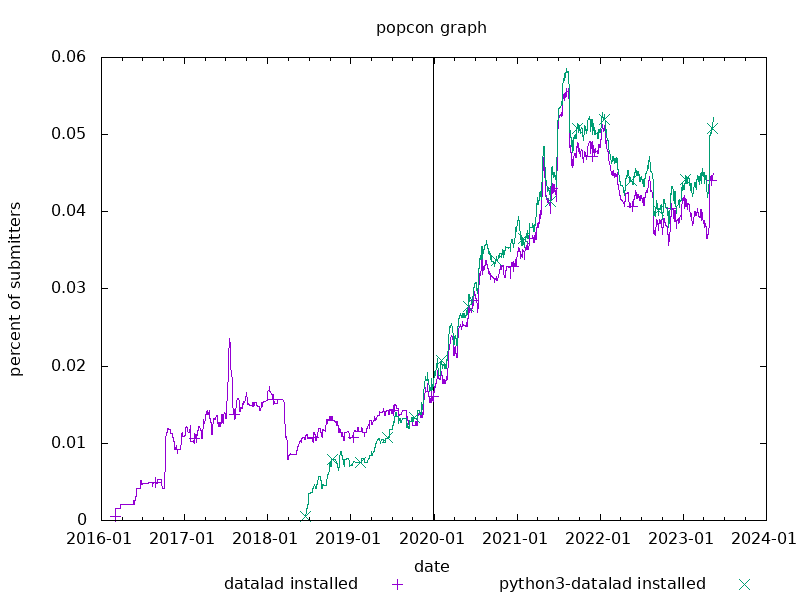
\includegraphics[width=.8\textwidth]{popcon-datalad.png}
	\caption[Debian package popularity counts for DataLad]{Popularity of the Debian packages DataLad and python3-datalad over time, expressed in percent of users that installed the package from the total amount of users submitting download statistics. January 2020 marks the first release of the Handbook as an accompanying user guide. Source: Debian Popcon, May 2024}
	\label{fig:popcon}
\end{figure}

\pagebreak


% !TeX root = ../main-english.tex
% !TeX spellcheck = en-US
% !TeX encoding = utf8
% -*- coding:utf-8 mod:LaTeX -*-

%This smart spell only works if no changes have been made to the chapter
%using the options proposed in preambel/chapterheads.tex.
\setchapterpreamble[u]{%
	\dictum[Ian Holmes, in an \href{https://twitter.com/ianholmes/status/288689712636493824}{\#overlyhonestmethods tweet}]{You can download our code from the URL supplied. Good luck downloading the only	postdoc who can get it to run, though.}
}


\chapter{Ensuring computational reproducibility across computational environments}
\label{chap:k3}

% from NISO: Beyond their potential to mitigate transparency and reproducibility issues, these practices provide important benefits for individual researchers by increasing exposure, reputation, chances of publication, number of citations, media attention, potential collaborations, and position and funding opportunities (Allen and Mehler, 2019; McKiernan et al., 2016; Nosek et al., 2022; Markowetz, 2015; Hunt, 2019).
Partially fueled by external incentives or requirements \citep{mckiernan2016open} \citep{dfg}, research curricula founded within the Open Science Movement \citep{munafo2017manifesto} \citep{poldrack2017scanning}, and a growing ecosystem of openly available infrastructure and tools \citep{NISO2022119623}, practices of publishing reproducibly are becoming more frequent.
Widespread sharing of code and data allows researchers to verify, reuse, and improve upon past work \citep{borghi2018data}.
Grass-roots movements such as Reprohack (\href{https://www.reprohack.org/}{www.reprohack.org}) or the ``Ten Years Reproducibility Challenge'' (\href{https://rescience.github.io/ten-years/}{rescience.github.io/ten-years}) train researchers to check published studies for reproducibility.
Consequently, attempts to reproduce previous studies often happen in different computational environments than those that originally created the results in question.
Ensuring computational reproducibility across computational environments is, however, a difficult technical challenge.
This following chapter outlines first its challenges, particularly in the field of neuroimaging, then its opportunities, and lastly an implementation to ensure computational reproducibility across computational environments.
Parts of this chapter were published as \citet{wagner2022fairly}: ``FAIRly big: A framework for computationally reproducible processing of large-scale data'' and are appropriately marked as such.


\section{The origins of reproducibility}

% from NISO: psychology (Open Science Collaboration, 2015; Klein et al., 2018), social sciences (Camerer et al., 2016, 2018), neuroimaging (Munafò et al., 2017; Botvinik-Nezer et al., 2020; Li et al., 2021), preclinical cancer biology research (Errington et al., 2021; Errington et al., 2021), and more (Hutson, 2018; Nissen et al., 2016; Serra-Garcia and Gneezy, 2021).
Over the past decade, interest in reproducibility has been fueled by salient failures to reconfirm published results in numerous fields, from psychology \citep{open2015estimating}, to biomedical imaging \citep{wagner202310}, to artificial intelligence \citep{hutson2018artificial}, or econonmics \citep{camerer2016evaluating}, often termed \textit{reproducibility crises}.
However, proposals to increase reproducibility, transparency, and robustness of science were made independently in various disciplines long before the current trend, in some cases dating back several centuries (maybe Robert Boyle, chemistry CITATION NEEDED).
Even the field of \textit{computational reproducibility} originated already more than 30 years ago in the field of seismology \citep{claerbout1992electronic} \citep{buckheit1995wavelab}, despite increased usage of the term in scientific literature only from 2015 onward (see \cref{fig:ngram}).
Consequently, the terminology around reproducibility has varied considerably over the years and across domains, and there is no universally agreed upon standardization of terminology in place yet \citep{barba2018terminologies}.
To disambiguate between several conflicting definitions of terms around reproducibility that are in active use, we shall define the terms used in this thesis as follows:

\subsubsection{Reproducibility}

Following the definition of \citet{peng2006}, \textit{reproducibility} refers to the practice of verifying a published result with the same methods and materials used by the original authors.

\subsubsection{Replicability}

\textit{Replicability}, on the other hand, refers to strengthening scientific evidence in favor of a result when ``multiple investigators [find similar results] using independent data, analytical methods, laboratories, and instruments''  \citep{peng2006}.

\subsubsection{Computational Reproducibility}

\textit{Computational reproducibility}, finally, matches the definition put forward in the 2019 report on ``Reproducibility and Replicability in Science'' by the National Academies of Science, Engineering and Medicine \citep{engineering2019reproducibility}: ``We define reproducibility to mean computational reproducibility – obtaining consistent computational results using the same input data, computational steps, methods, code, and conditions of analysis''.


\begin{figure}
	\centering
	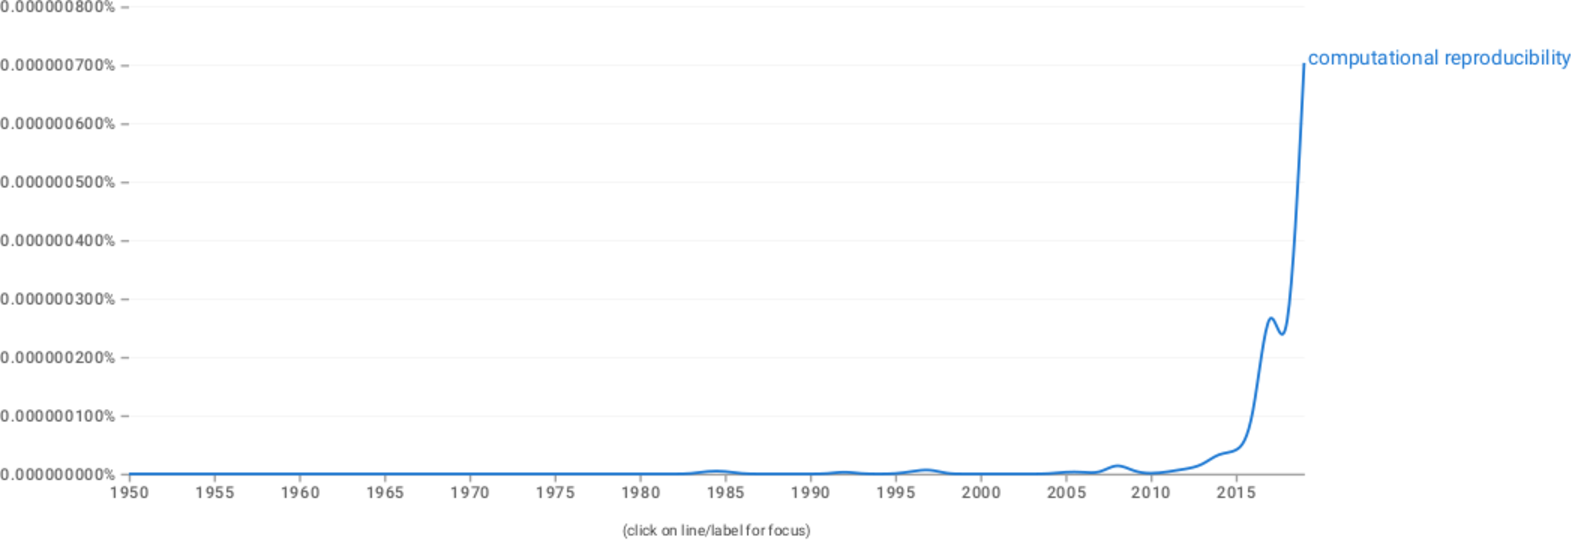
\includegraphics[width=\textwidth]{google_ngram_reproducibility_2023-05-08.pdf}
	\caption[Computational reproducibility in the literature]{Popularity of computational reproducibility: A chart of the frequencies of the n-gram ``computational reproducibility" (using yearly count, normalized be the numbers of publications in each year) in literature included in the English(2019) corpus of Google books. This graph has been created using the Google Ngram Viewer (\href{https://books.google.com/ngrams/info}{books.google.com/ngrams}) \citep{michel2011quantitative}}
	\label{fig:ngram}
\end{figure}


\subsection{``Everything matters'' for computational reproducibility in neuroimaging}

% maybe NARPS paper?`

The building blocks of research output extend to more than the files that constitute the actual research output, but also to all elements involved in its generation \citep{claerbout1992electronic}.
Consider different types of research output:
Raw data originates from acquisitions based on - potentially ongoing - experiments, raw data transformations, or data cleaning.
Processed data or results stem from computations with analysis code or software in specific versions on particular data.
And software, expressed in raw (code) or derived (transformed into executable) form, is created or used in specific computational environments, with compilers, underlying libraries, and systems in distinct versions.
Consequently, these building blocks play an integral part in the genesis of research outputs, and changes in these building blocks or their composition can translate to changes in the resulting research output.\\

The complexity in neuroimaging studies makes reproducibility non-trivial:
The details of how code, software, or data have been used to generate a research output, such as analysis parameterization, the subset of data used as input, or sequence and invocation of employed software tools, are volatile.
A study of data availability, reusability, and reproducibility demonstrated that well-described, ``in principle reusable'' data often does not suffice to reproduce the scientific findings of the corresponding publications due to  missing process provenance metadata \citep{hardwicke2018data}.


The fact that different neuroimaging software tools can produce distinct results from the same data despite using similar conceptual methodology is well known \citep{bowring2019exploring}.
This has been attributed to implementation differences (CITATION NEEDED), software errors \citep{eklund2016cluster}, or analytic configurations.
For example, in task-based fMRI, \citet{li2021moving} found that the choice of output space or resolution can have a marked impact on variability between conceptually similar processing pipelines.
Surprising result variability can also occur when the same data is analyzed repeatedly with the same processing pipeline, but minor variations in parametrization. \citet{mueller2017commentary} reported that the choice of resampling resolution impacts alpha inflation, and \citet{li2021moving} identified the decision whether or not to include global signal regression as a major source of intra-pipeline variation.
But also different operating systems, or differences in versions of a singular software tool or operating system can result in different outcomes of the same analysis \citep{gronenschild2012effects} \citep{glatard2015reproducibility}.
%more here
Computational reproducibility across computing environments thus often remains elusive unless accounted for from the very start.
Therefore, in addition to ``Everything matters'',  \citet{kennedy2019everything} cued the phrase ``Reproducible by Design (as opposed to reproducibility as an afterthought)'' for conducting research in a way that makes computational reproducibility possible.
The next section highlights a number of strategies for this, and how reproducibility is tied to research data management.

% However, a growing number of studies suggest that differences in the implementation of these processing steps or how they are “glued together” can yield notably different outcomes. Studies systematically comparing specific preprocessing steps such as segmentation15, motion correction16, and registration17–19 have reported substantial variation in outputs generated across independently developed packages when applied to the same data. In the analysis of task fMRI data, end-to-end pipelines built using different software packages have been found to produce marked variation in the final results20–23. from https://www.biorxiv.org/content/10.1101/2021.12.01.470790v2.full


\section{Towards re-usable research objects}


The reusability of research objects has become a distinct characteristic of scientific practice as it allows for reproduction, verification, building up upon and extending existing work, evidence synthesis, and minimizing duplicate efforts in the advancement of science \citep{thanos2017research}.
With this, it maximizes the impact of the funding and work that resulted in the research output.
Therefore, it is considered the “ultimate goal” of the FAIR principles \citep{wilkinson2016fair}, and an explicit and central expectation in a variety of funding sources such as the Economic and Social Research Council (ESRC, UK), the European Research Council (ERC, EU), or the National Institutes of Health (NIH, US).
In the scope of the FAIR principles, reusability focuses on the ability of a human or a machine to decide if data are useful and usable in a particular context based on richly curated metadata.
This reusability requires trust \citep{bechhofer2010research}. Re-users must be able to audit the steps performed in an experiment or analysis in order to be convinced of the validity of the results or derivatives.
FAIR principle R1.2, ``(Meta)data are associated with detailed provenance'' \citep{wilkinson2016fair}, refers to this.
Where resources are not fully FAIR yet, manual reproducibility typically provides this form of trust: for example when a new student checks if the previous findings that a their project builds up on still hold.\\

Many scientific fields or projects argue that FAIRness requires coordinated use of ontologies for metadata and brought forward efforts for ontology development and consensus building (e.g., \citep{wise2019implementation}, \citep{abrams2022standards}, \citep{papadiamantis2020metadata}), but not in all domains are the necessary metadata standards incentivized or ready to use.
A few years before the publication of the FAIR principles, \citet{bechhofer2013linked} cued the term "reusable research object" in a conceptual position paper, and defined it as a ``container for a principled aggregation of resources, produced and consumed by common services and shareable within and across organisational boundaries. [...It] includes not only the data used, and methods employed to produce and analyse that data, but also the people involved in the investigation. An association with a dataset (or service, or result collection, or instrument) is now more than just a citation or reference to that dataset (or service or result collection). The association is rather a link to that dataset (or service or result collection) that can be explicitly followed or dereferenced providing access to the actual resource and thus enactment of the service, query or retrieval of data, and so on.''
% Detail how datalad adheres to these requirements.
In the following, I will highlight four properties of DataLad dataset or its contents that make them a reusable research object \citep{wagnerohbm2021}, and argue why the \gls{rdm} features that DataLad provides assist with FAIRification.

\subsubsection{Versioned}

The information ``I generated X from data Y with software Z'' is insufficient for reproducibility and trustworthiness if Y exists in multiple versions or subsets, if different releases of Z have relevant implementation differences, or if Z behaves differently depending on the environment it is used in.
The first relevant feature is version control for all relevant files -- from data to code to software environments.
If digital research objects are tracked, they can be accessed and used transparently in a uniquely identified version state, and this exhaustive identity registration removes ambiguity that arises if the files in question are not completely static.
DataLad Datasets provide such versioning for any digital file.
This lays the foundation for exhaustive tracking \\



Tracking can be applied with different levels of granularity, e.g., for each conceptually important step, or covering a complex transformation at once, but in both cases unambiguous identification of starting state, transformation, and end state is needed.

\subsubsection{Actionable}


The most pragmatic approach to capture metadata is at the time of their creation, with the tools and persons that are involved in the creation of research outputs anyway \citep{dallas2016digital}.
Compared to post-hoc reconstruction, immediate metadata curation by expert actors has advantages even if it does not conform to an eventual ontology yet. For one, it can be detrimental for metadata quality if the information isn’t supplied at the point in time or by the actors that have maximal knowledge - anything not carefully recorded can be easily forgotten \citep{gryk2019foregrounding}.
Annotating research outputs only after their creation is tedious, often without an immediate benefit for curators, rarely explicitly incentivized \citep{edwards2011science} \citep{san2009long}, and thus easily swept under the table
But while early curation can increase the comprehensiveness of metadata, additional measures should guarantee its validity, as even fully described research outputs fail to be reproducible or reusable if their description or provenance contains errors (see, e.g. \citep{manninen2017reproducibility}).
The most pragmatic approach to valid metadata is to base subsequent processing on them.
In the simplest case, this can be a codified parametrization of an analysis in a configuration or analysis design file (see e.g., \citep{jas2018reproducible}).
If an analysis based on the file completes successfully, it constitutes valid provenance metadata, created by an expert or automatically at the earliest possible time at no additional cost.
It also adds immediate benefit for curators as it captures relevant provenance and detects erroneous or missing metadata in passing.
This process is easiest if the tools used during the creation of a research output use the same metadata that gets eventually published alongside the final research output.
Even if this metadata does not follow established community standards yet, it preserves knowledge that would otherwise be lost, without requiring additional training, impeding later additions, or putting additional burden on scientists - it is a byproduct of standard scientific practice.
FAIRness is not a fixed state, but a maturation process where digital objects are rendered increasingly self-descriptive to the machine \citep{wilkinson2019evaluating}.
Ensuring actionable metadata, i.e., metadata that is cheaply acquired, validated by experts, simply structured, and machine-readable to relevant tools in the evolution of a research output, supports this process.
The simpler such actionable metadata are structured, the lower the barrier to aggregate them, and the easier it is to read or transform them into an eventual ontology or metadata standard.
The earlier metadata are captured, the more structured and comprehensive they are, the more useful they are to their creators, and the more time there is to ensure their validity via direct use.


\subsubsection{Modular}

The reusability of scientific work can improve if it is accessible in modular units that constitute unambiguous multi-use components, such as raw data, processed data, or software. Generally speaking, we refer to modularization as any process that structures data into distinct units. In the simplest case, this means placing conceptually distinct content into separate files, and grouping files in individual directories to reflect more global structures. Modularization into distinct units, such as the directories “code/” and “inputs/”, increases transparency if each location is associated with distinguishable content, flexible recombination of such components into new projects, continuous evolution of an individual module without impact on other components of a project, and location-specific access control. Different rules of thumb can guide the decision to modularize. One is different target audiences, e.g., when two research outputs cater to the needs of separate consumer populations (raw data versus aggregated results), if they are available at different confidentiality levels (personal versus anonymous data), or if the utility of the data depends on different amounts of domain knowledge or access (data in proprietary formats versus conversions to open file formats). Modularization is also useful if research outputs underlie a different evolutionary pace, e.g., “factual” data like measurements versus subsequent processing flavors, or a single acquisition in longitudinal or large-scale studies versus the final dataset that eventually encompasses all acquisitions. Technical constraints can constitute a reason, too. The UKBiobank (www.ukbiobank.ac.uk) collects data from 500.000 participants, but a directory hierarchy with 500,000 subdirectories exceeds the limits of some file systems, warranting modularization. While modularization is a standard data management strategy to reduce clutter, project complexity may impede or blur it accidentally. Consider an analysis that saves computed derivatives next to input data instead of a distinct output location: input-output relations aren’t necessarily intuitive anymore without domain or project knowledge. In a modular approach, inputs and outputs remain clearly dissociatable in separate units.
At first glance, modularization may appear contradictory to the first trait. A single modular unit can not entail all relevant elements of a scientific study or data analysis if it should facilitate reuse within and outside its original purpose. In order to achieve exhaustive tracking of all elements without sacrificing modularity, multiple modular units must be linkable in dependency relationships.
A useful metaphor are package management systems such as conda or APT: A software package is a modular unit, installed with a package manager. However, packages usually depend on other software packages, which are listed as its “dependencies”. During installation, package managers check if all of the linked dependencies exist on the system, and if not, install them in the required versions automatically. In scientific projects, modular units (data, software, code) are the dependencies of a given research output. When those units are tracked, dependency relationships can include precise versions. Beyond transparency and tidiness, modularization and linkage thus provide methods for reuse with which stand-alone units can be assembled into new projects, and research output contains the pieces it was derived from as linked dependencies.


\subsubsection{Portable}

The more portable a digital research object is, the easier it is to reuse it.
A research object is fully portable if no adjustments are necessary for it to function the way it is intended to on different computational infrastructure, and ultimate portability is achieved if it can be used by a naive re-user with a different area of expertise (i.e., without domain knowledge).
The more adjustment or domain knowledge is necessary, the less portable a research output becomes. An openly shared computational pipeline is not fully portable if its invocation requires expert knowledge, licenses, or proprietary data structures, an openly shared dataset is not fully portable if a re-user has to invest many hours into data wrangling


\begin{figure}
	\centering
	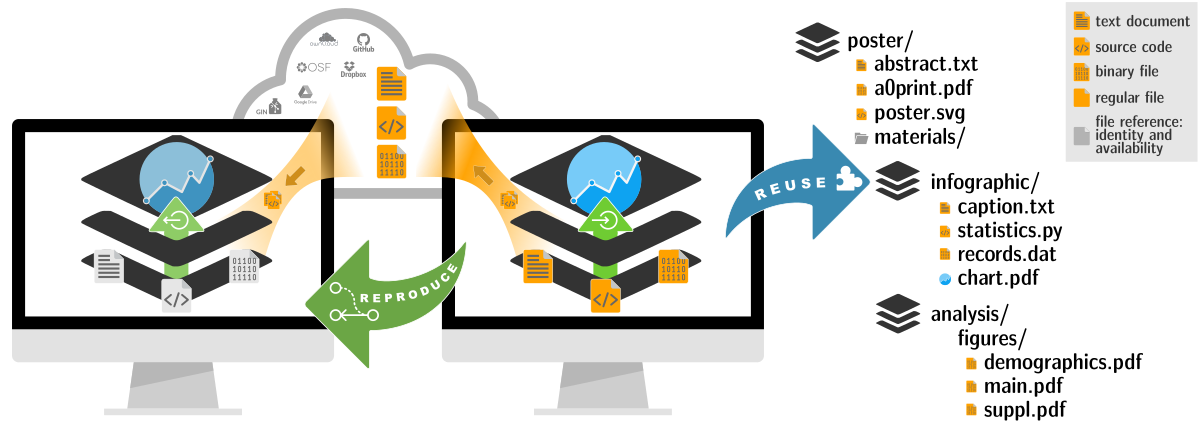
\includegraphics[width=.9\textwidth]{vamp.png}
	\caption[DataLad datasets as reusable research objects]{Reusing research outputs implies trust, and trust should be earned through verification. Verification is enabled by provenance information. Provenance capture of research outcomes requires exhaustive tracking of all inputs, as well as process records that describe how inputs were combined and transformed to generate outputs (middle). When lightweight metadata are actionable, they can be used to reproduce research outputs in a different environment from precisely identified inputs by (re-)applying the recorded process (left). A data structure that affords this type of portable recomputation is a self-contained unit that can be reused as a modular input component for incremental research (right).
	}
	\label{fig:vamp}
\end{figure}




% curation needs to be pragmatic

Although FAIR research objects are universally desirable, in practice, the necessary standards and procedures for creating FAIR (meta)data are not always already in place when research is conducted.
This can turn FAIRification into a bureaucratic data governance effort, diminishing the immediately obvious benefits for the curator \citep{zehl2016handling}.


The next section details a technical implementation and proof-of-concept analysis to create such reusable research objects as a byproduct of \gls{rdm} in analyses of any scale.





One way to track digital files is
While it is possible to exhaustively track all elements involved in a project with version control, industry use differs from RDM demands in science.
In industry contexts, it is primarily employed in software engineering for small-sized text files (source code). Science often works with large amounts of potentially sizable or binary files.
To exhaustively track all elements involved in a scientific project, large and binary files such as data and computational environments need to be versioned, too.
The concept of software containers - portable, light-weight software environments - make it possible to encapsulate computational environments as in-principle trackable elements, and a range of tools provide the ability to track even terabyte-sized and binary files.
Overall, version control is a well-established and reliable tool in industry and science. It can be employed at any point during a project, and yields a hands-on digital notebook of a project.
By extending its use beyond small-sized files to any digital research outputs and everything involved in its generation, version control can not only constitute established and beneficial research data management, but also lay the foundation for reusability by exhaustively tracking relevant digital elements and making them identifiable in precise versions.

From Donoho Buckheit 2015: Performance has everything to do with specifics: exactly what was done (which wavelets,
which coders, which detectors, which corpus of data) with exactly what parameters. In
this setting, publishing figures or results without the complete software environment could
be compared to a mathematician publishing an announcement of a mathematical theorem
without giving the proof. Waveleticians ought to publish their complete computational
environments


As highlighted in the Introduction, digital research outputs are the by- or end-products of scientific studies or analyses, from code, software, raw data or processed data, to analysis results or papers.

\pagebreak

\section{FAIRly big: A framework for computationally reproducible processing of large-scale data}

% role of sample size for reproducible results: \citep{li2021moving}

%  \citep{li2021moving} "highlight the reality that as the test-retest reliability approaches optimal levels for laboratory measurement, pipeline implementation differences will impose an inherent upper bound on the agreement of preprocessed data. These findings also underscore that 10 minutes of data, which has been common in the field until at least recent years, are insufficient for producing results that are reliable enough to reveal substantive pipeline-related variation."

\begin{figure}
	\centering
	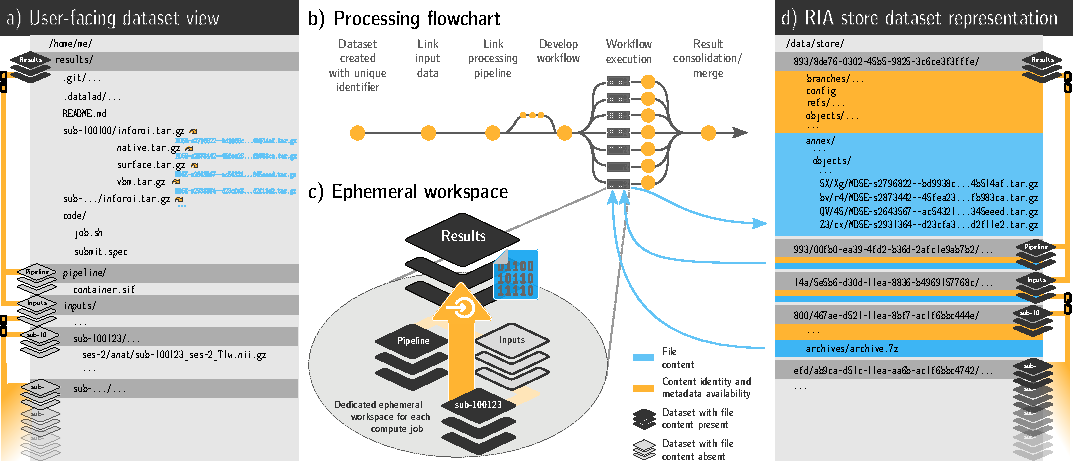
\includegraphics[width=\textwidth]{ukbworkflow_simplified.pdf}
	\caption[]{}
	\label{fig:fairly_workflow}
\end{figure}

\begin{figure}
	\centering
	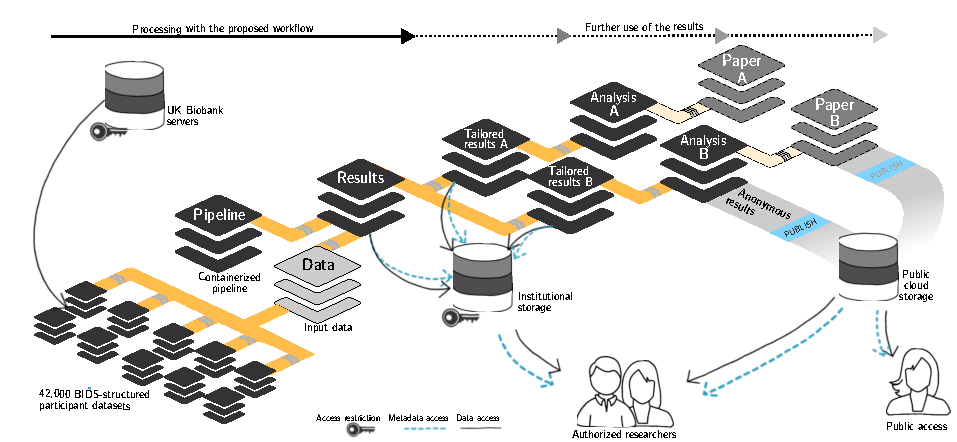
\includegraphics[width=\textwidth]{ukb_datasets.pdf}
	\caption[]{}
	\label{fig:fairly_datasets}
\end{figure}

\begin{figure}
	\centering
	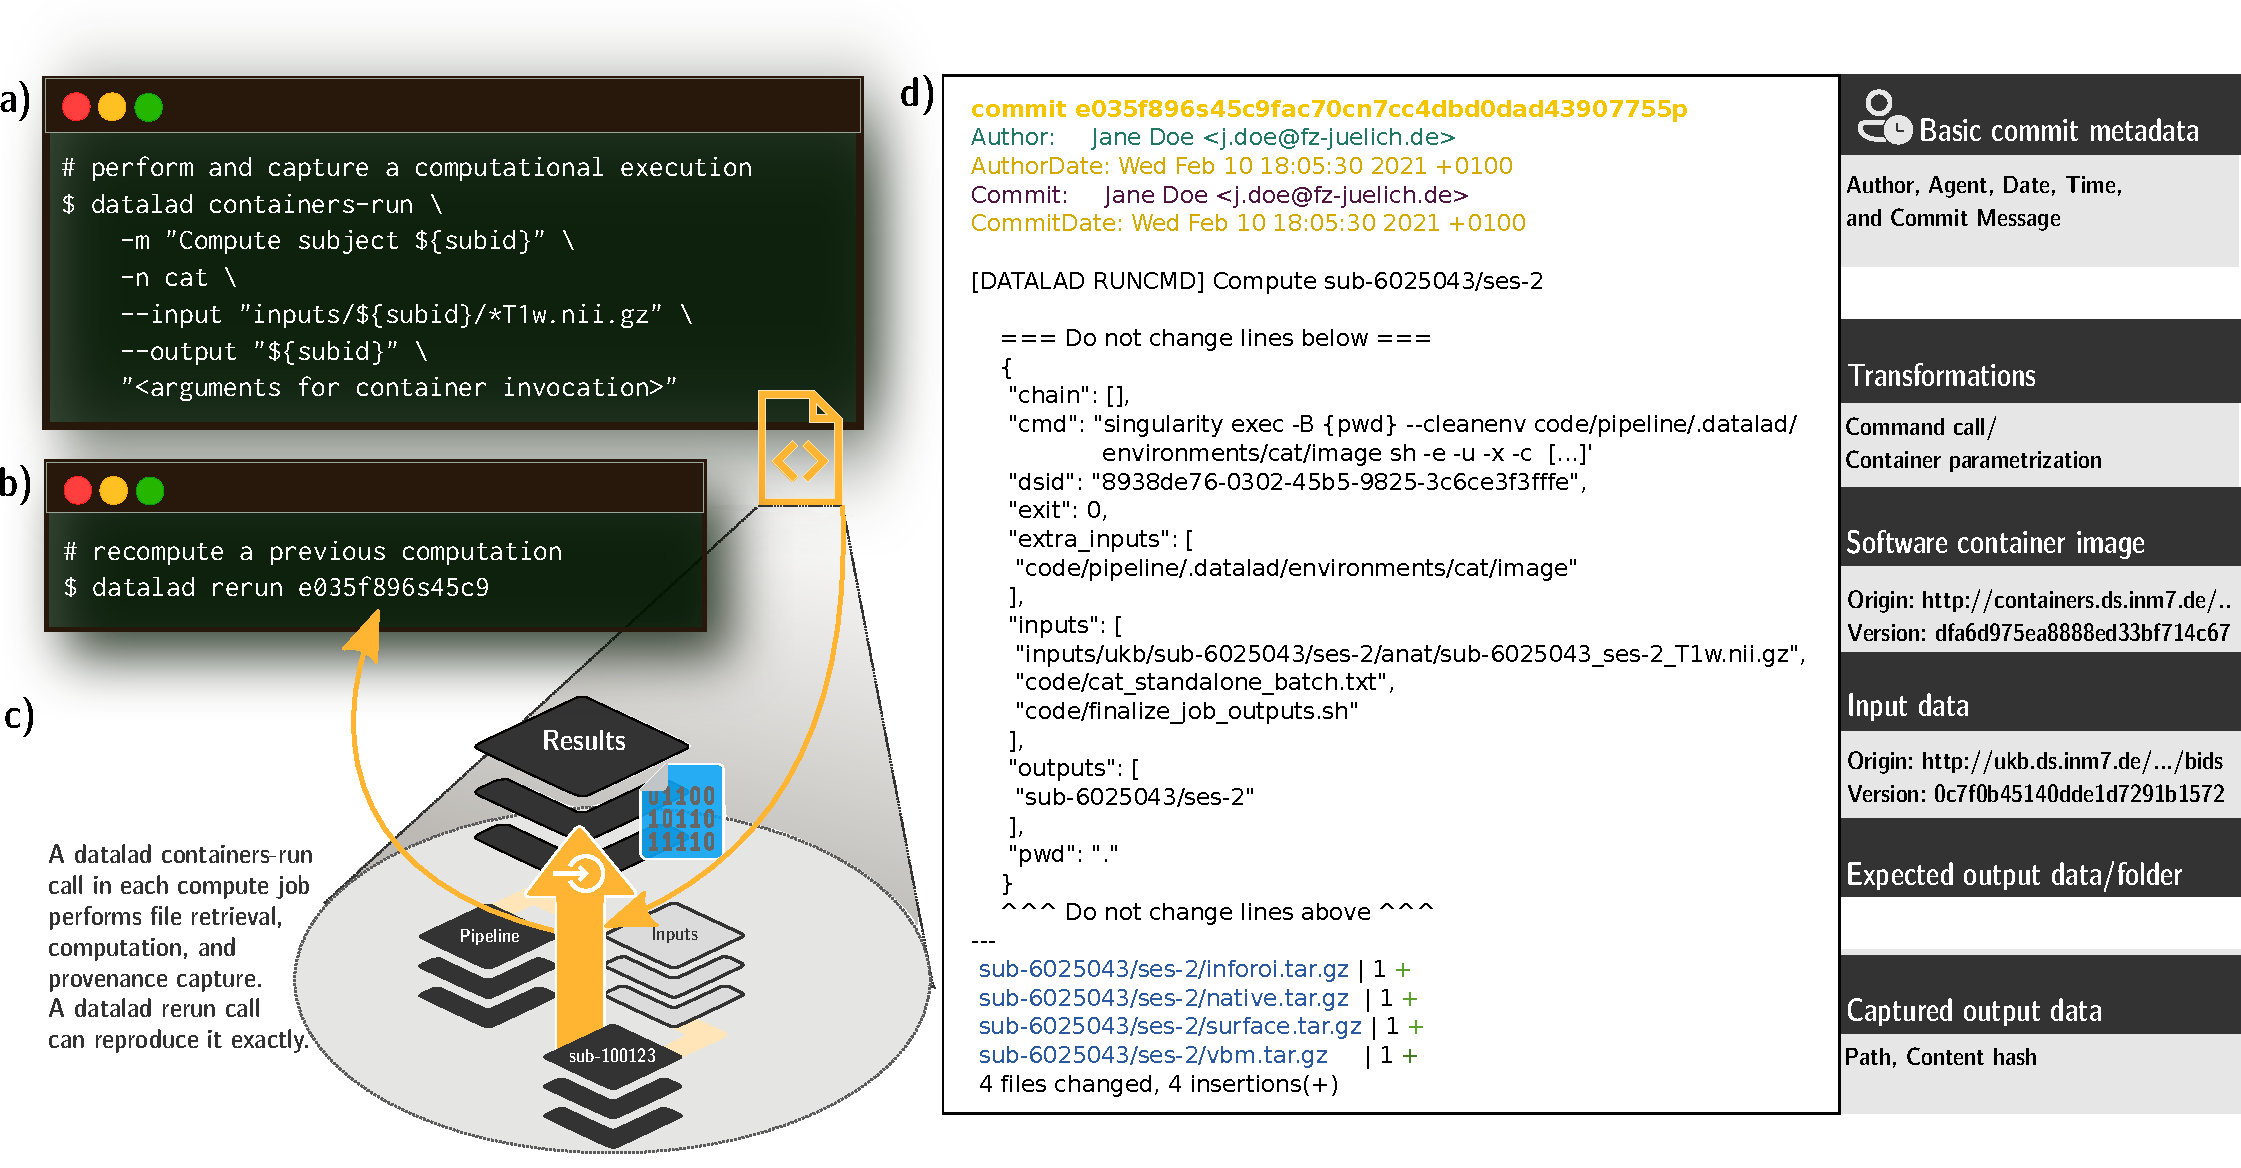
\includegraphics[width=\textwidth]{coarsemetadata.pdf}
	\caption[]{}
	\label{fig:fairly_metadata}
\end{figure}

% on re-analyzing the pipeline, cite li2021moving: "we demonstrated the role that pipeline replication can play as a means of exploring analytic variation and assessing the robustness of findings. To this end, we leveraged and extended the flexibility of C-PAC to replicate non-MATLAB dependent minimal processing pipelines (ABCD-BIDS, CCS, fMRIPrep-LTS) in a single platform"


\pagebreak
% !TeX root = ../main-english.tex
% !TeX spellcheck = en-US
% !TeX encoding = utf8
% -*- coding:utf-8 mod:LaTeX -*-

%This smart spell only works if no changes have been made to the chapter
%using the options proposed in preambel/chapterheads.tex.
\setchapterpreamble[u]{%
	\dictum[Isaac Newton]{If I have seen further it is by standing on the shoulders of Giants}
}

\chapter{Maybe Magma? Computational cognitive neuroscience?}
\label{k4}

Look mom, some text!

\pagebreak


% !TeX root = ../main-english.tex
% !TeX spellcheck = en-US
% !TeX encoding = utf8
% -*- coding:utf-8 mod:LaTeX -*-

%This smart spell only works if no changes have been made to the chapter
%using the options proposed in preambel/chapterheads.tex.
\setchapterpreamble[u]{%
	\dictum[Albert Einstein]{If we knew what it was we were doing, it would not be called research, would it?}
}

\chapter{Reproducibility in exploratory data analyses}
\label{k5}

The previous chapters focused on the technical challenges of reproducibility management, especially when applications need to scale to large samples.
However, a different common difficulty is to ensure reproducibility and maintain good research data management routines when the to be undertaken analyses are not entirely mapped out from the start, and a research project is exploratory in nature.
Even if an analysis project does not yield a published article as its final outcome, intermediate research outcomes are a valuable stepping stone for further research or researchers.
This upcoming chapter describes a data analysis project studying working memory in sequential decision making.

\section{Theoretical background}

%Rationale from Luka
In natural settings, value-based decisions under risk often have to be made without visual presence of competing alternatives.
Do I commit to buying the red bicycle in the store I'm currently in, or should I return to the previous bike shop and pick the blue one?
Do I want to rent the flat I viewed last Sunday, or the apartment I saw on Tuesday?
In such situations, the subjective value of alternative options has to be encoded, held in working memory through a maintenance (or ``delay'') period, and retrieved in order to form a categorical choice.

Numerous studies investigate the neural activity that persist throughout the delay period, and how it might represent relevant properties to subjective value.
\citet{roux2014working} proposed that gamma band oscillations of groups of neurons are generically involved in the maintenance of working memory.

However, \citet{pavlov2022oscillatory} highlighted the lack of agreement in the field in a systematic review recently.
However, the temporal dynamics of the decision process as well as the maintenance of different valued options in working memory are less thoroughly investigated questions.


\section{The MEMENTO study}


Therefore, the memento study investigated how decision-relevant information is retained in working memory using a decision making task with concurrent \gls{meg} acquisition.
It was acquired as part of the SFB 779 project B16N (``offline value representations in sequential decision making'') at the Otto-von-Guericke University Magdeburg in 2016 by \citet{kaiser}, and has not been previously published.
The following study overview adheres to the COBIDAS MEEG reporting guidelines for reproducible MEEG research \citep{pernet2020issues}.
The code used for preprocessing and analysis was bundled into a publicly available Python package \texttt{pymento\_meg} and is available from GitHub\footnote{\url{https://github.com/adswa/pymento_meg}} and \url{PyPi.org}.
Underlying software packages are listed in Table TODO.

\subsection{Participants}

$N = 22$ right-handed, healthy participants with normal or corrected-to-normal vision were recruited at the Center for Behavioral Brain Sciences and on the university campus Magdeburg.
Their mean age was 26 years, and 10 participants were male.
Handedness was assessed with the Edinburgh Handedness Inventory \citep{oldfield1971assessment}.
Participants gave their informed consent to participate in the study, and received a base monetary compensation in the order of 8€ per hour with a performance-dependent bonus of up to 3€.
Ethics approval was obtained from the University Clinic Magdeburg.

\subsection{Experimental design}

The experiment consisted of 510 trials, grouped into 5 blocks with a variable break in between.
Each trial required a decision between one of two stimulus options, presented as gabor patches on the left and right side of the screen (\cref{fig:memento_trial}).
Importantly, stimulus options were presented in succession, with a delay period through which the decision-relevant properties of the first stimulus had to be retained in working memory.
The number of stripes in the gabor patch encoded the reward magnitude (either 0.5, 1, 2, or 4 points), and the angle of stripes encoded reward probability (either 10\%, 20\%, 40\%, or 80\%): The more stripes, the higher the reward, and the larger the angle, the higher the probability.
\cref{fig:memento_stim} provides an overview.
Participants learned these associations in a tutorial prior to the experiment (\cref{fig:memento_tutorial}).
Each trial started with a fixation cross (1000-1900ms, jittered), followed by the first stimulus on the left side of the screen for 700ms, a 2000ms delay period through which the phrase ``or'' was presented in the center of the screen, the second stimulus option on the right side of the screen for 700ms, and a feedback screen.
Once the second stimulus option was displayed, participants chose the left or right option via a button press with the right or left index finger, respectively.
The feedback screen showed both options side by side with a frame around the chosen option, and revealed which option had been rewarded via color coding (red: unrewarded, green: rewarded).
If a decision was not made within 5 seconds, the trial was aborted and participants saw a message to respond faster.
A progress bar at the bottom of the screen tracked gains over time, resulting in a bonus payment whenever it hit a gold target line.
Participants were instructed to maximize their gains and to respond as fast as possible.
Stimulus presentation was controlled by Psychtoolbox \citep{kleiner2007s} running on Matlab 2012b (The Mathworks Company, Natick, MA).
All stimuli were presented on a grey background with a contrast optimized for the MEG recording chamber.
A photodiode, taped onto the stimulation screen, was used to determine visual stimulus onsets.
TODO: Add delay
In total, the experiment lasted approximately 60 minutes.

\begin{figure}
	\centering
	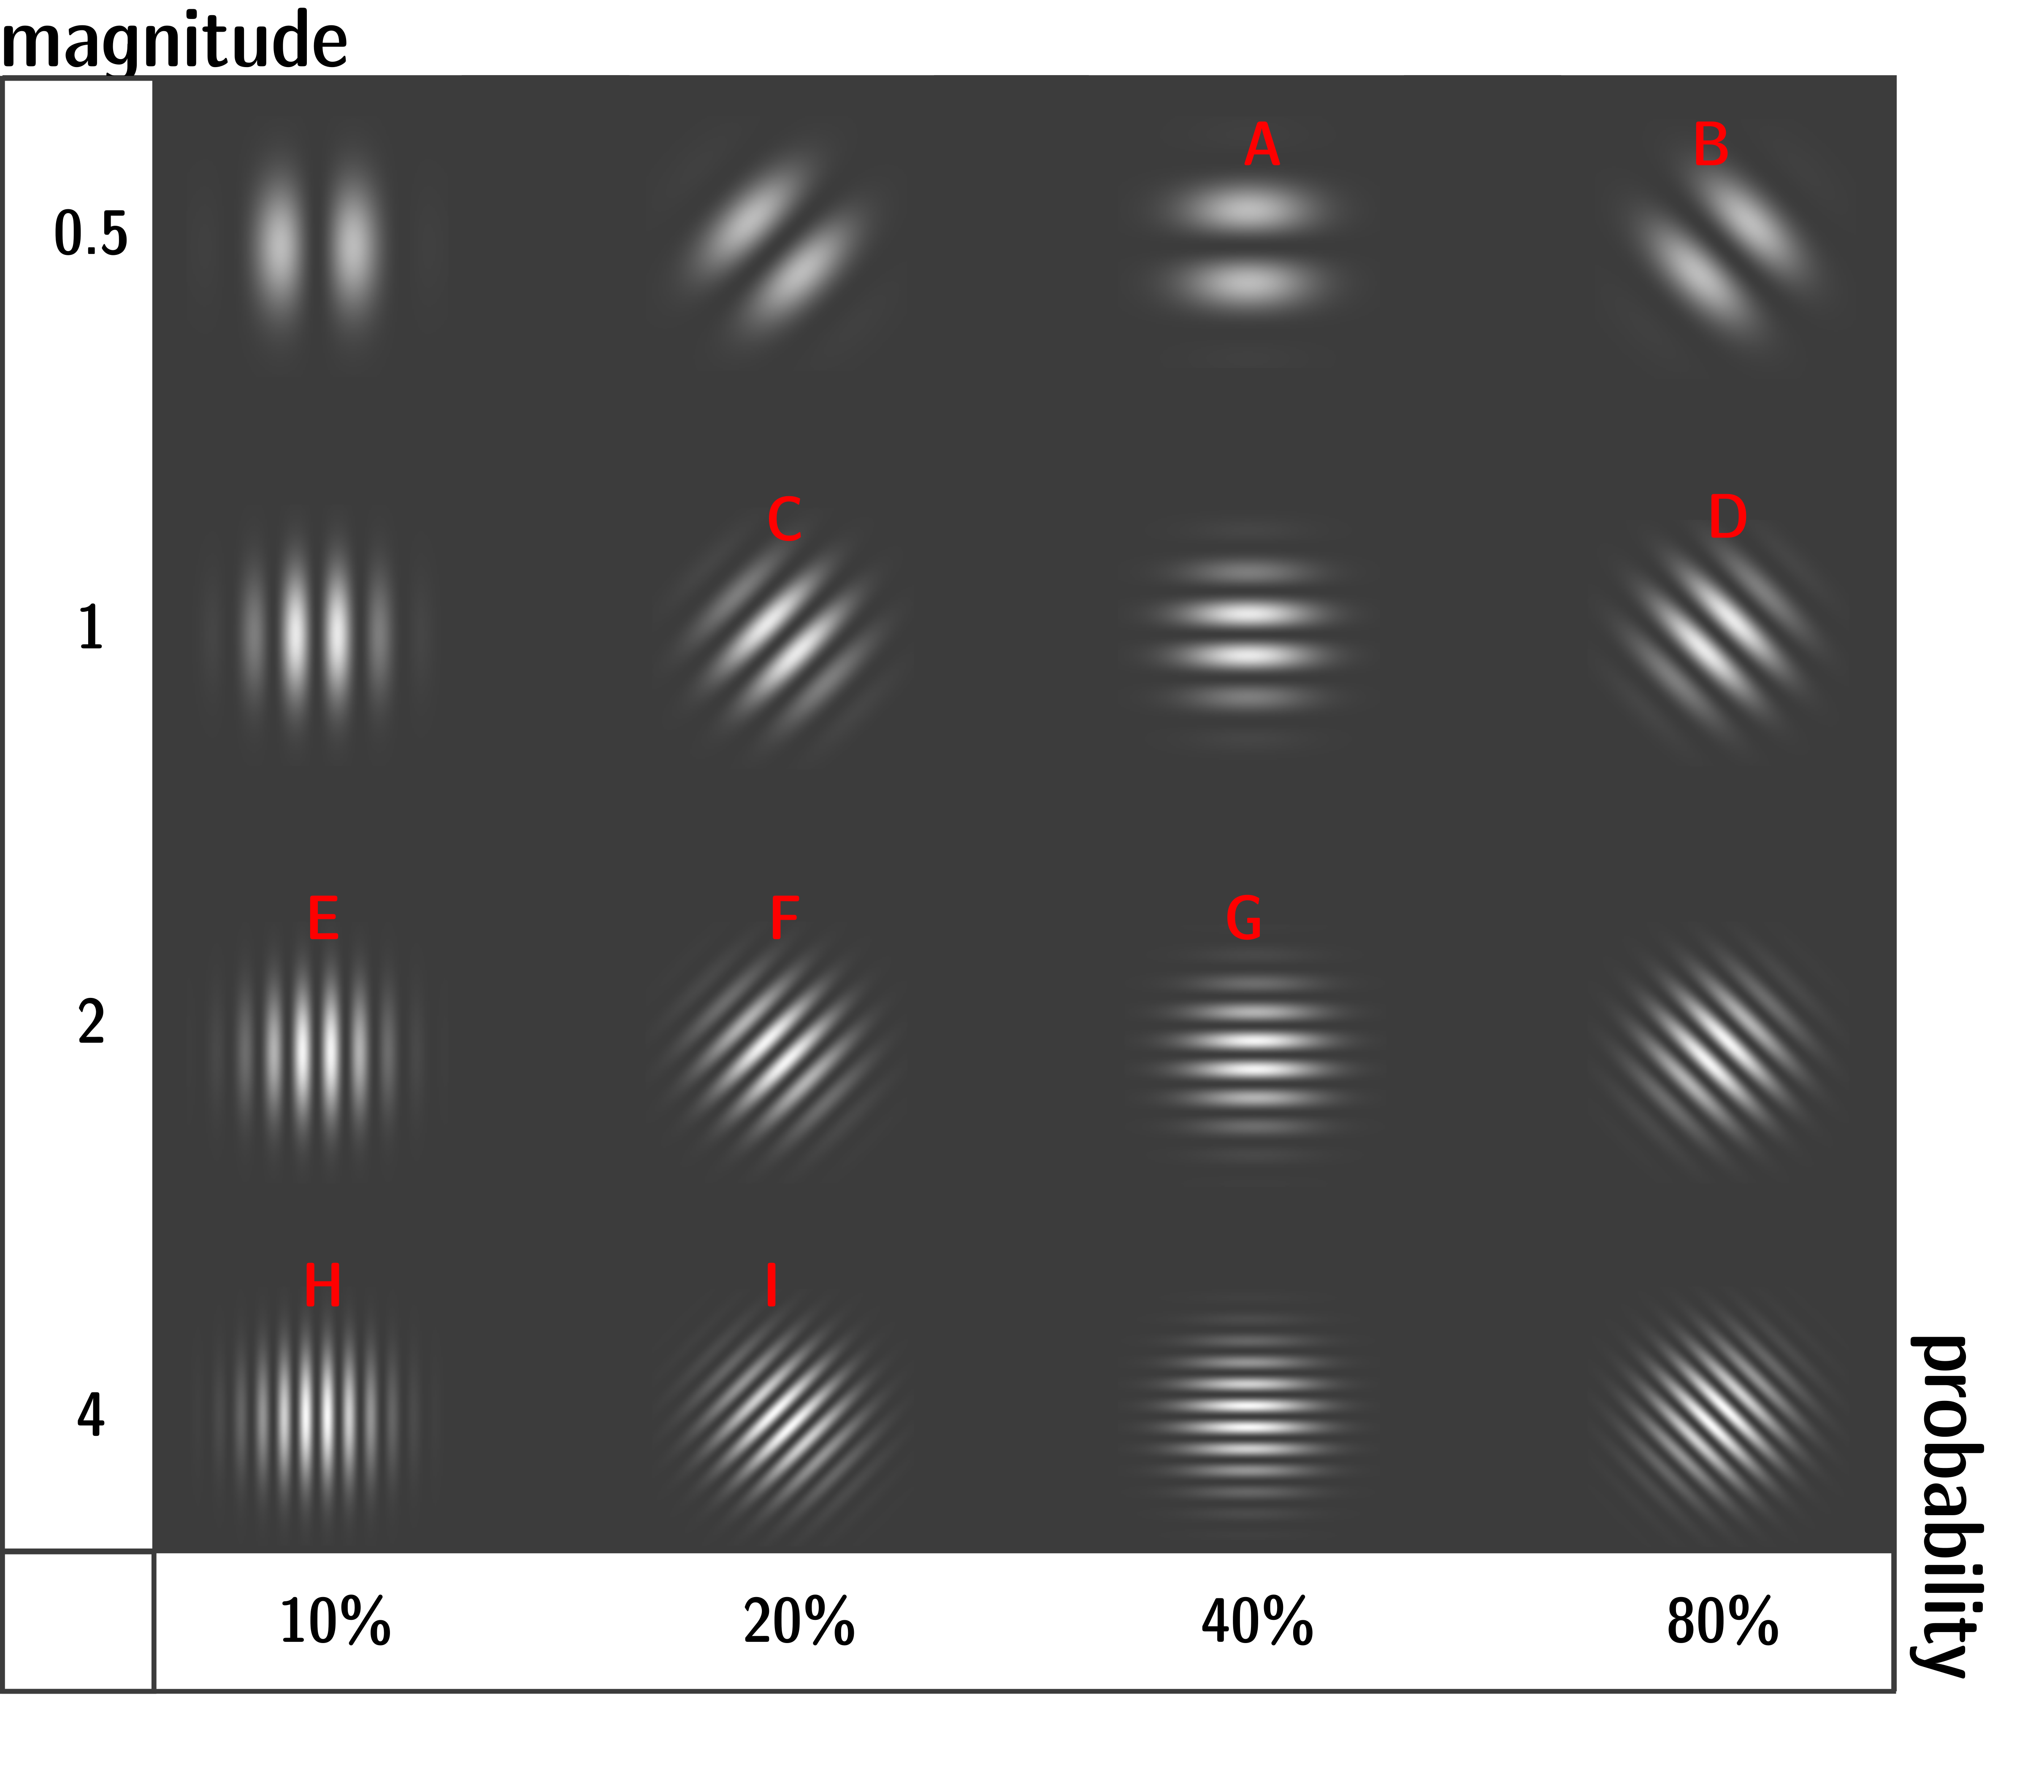
\includegraphics[width=0.5\textwidth]{memento/memento-stimuli.png}
	\caption[Stimulus overview]{Stimulus overview: Gabor patches varied in the number of stripes and their angle, encoding magnitude and probability, respectively. While all presented stimuli were learned in the tutorial, red letters indicate the selection of nine stimulus types used for the left option in the actual experiment. Trials without this annotation were only used intermittent as the right stimulus option to balance the overall expected value between the left and right stimulus option over the course of the experiment.}
	\label{fig:memento_stim}
\end{figure}

\begin{figure}
	\begin{subfigure}{.54\textwidth}
	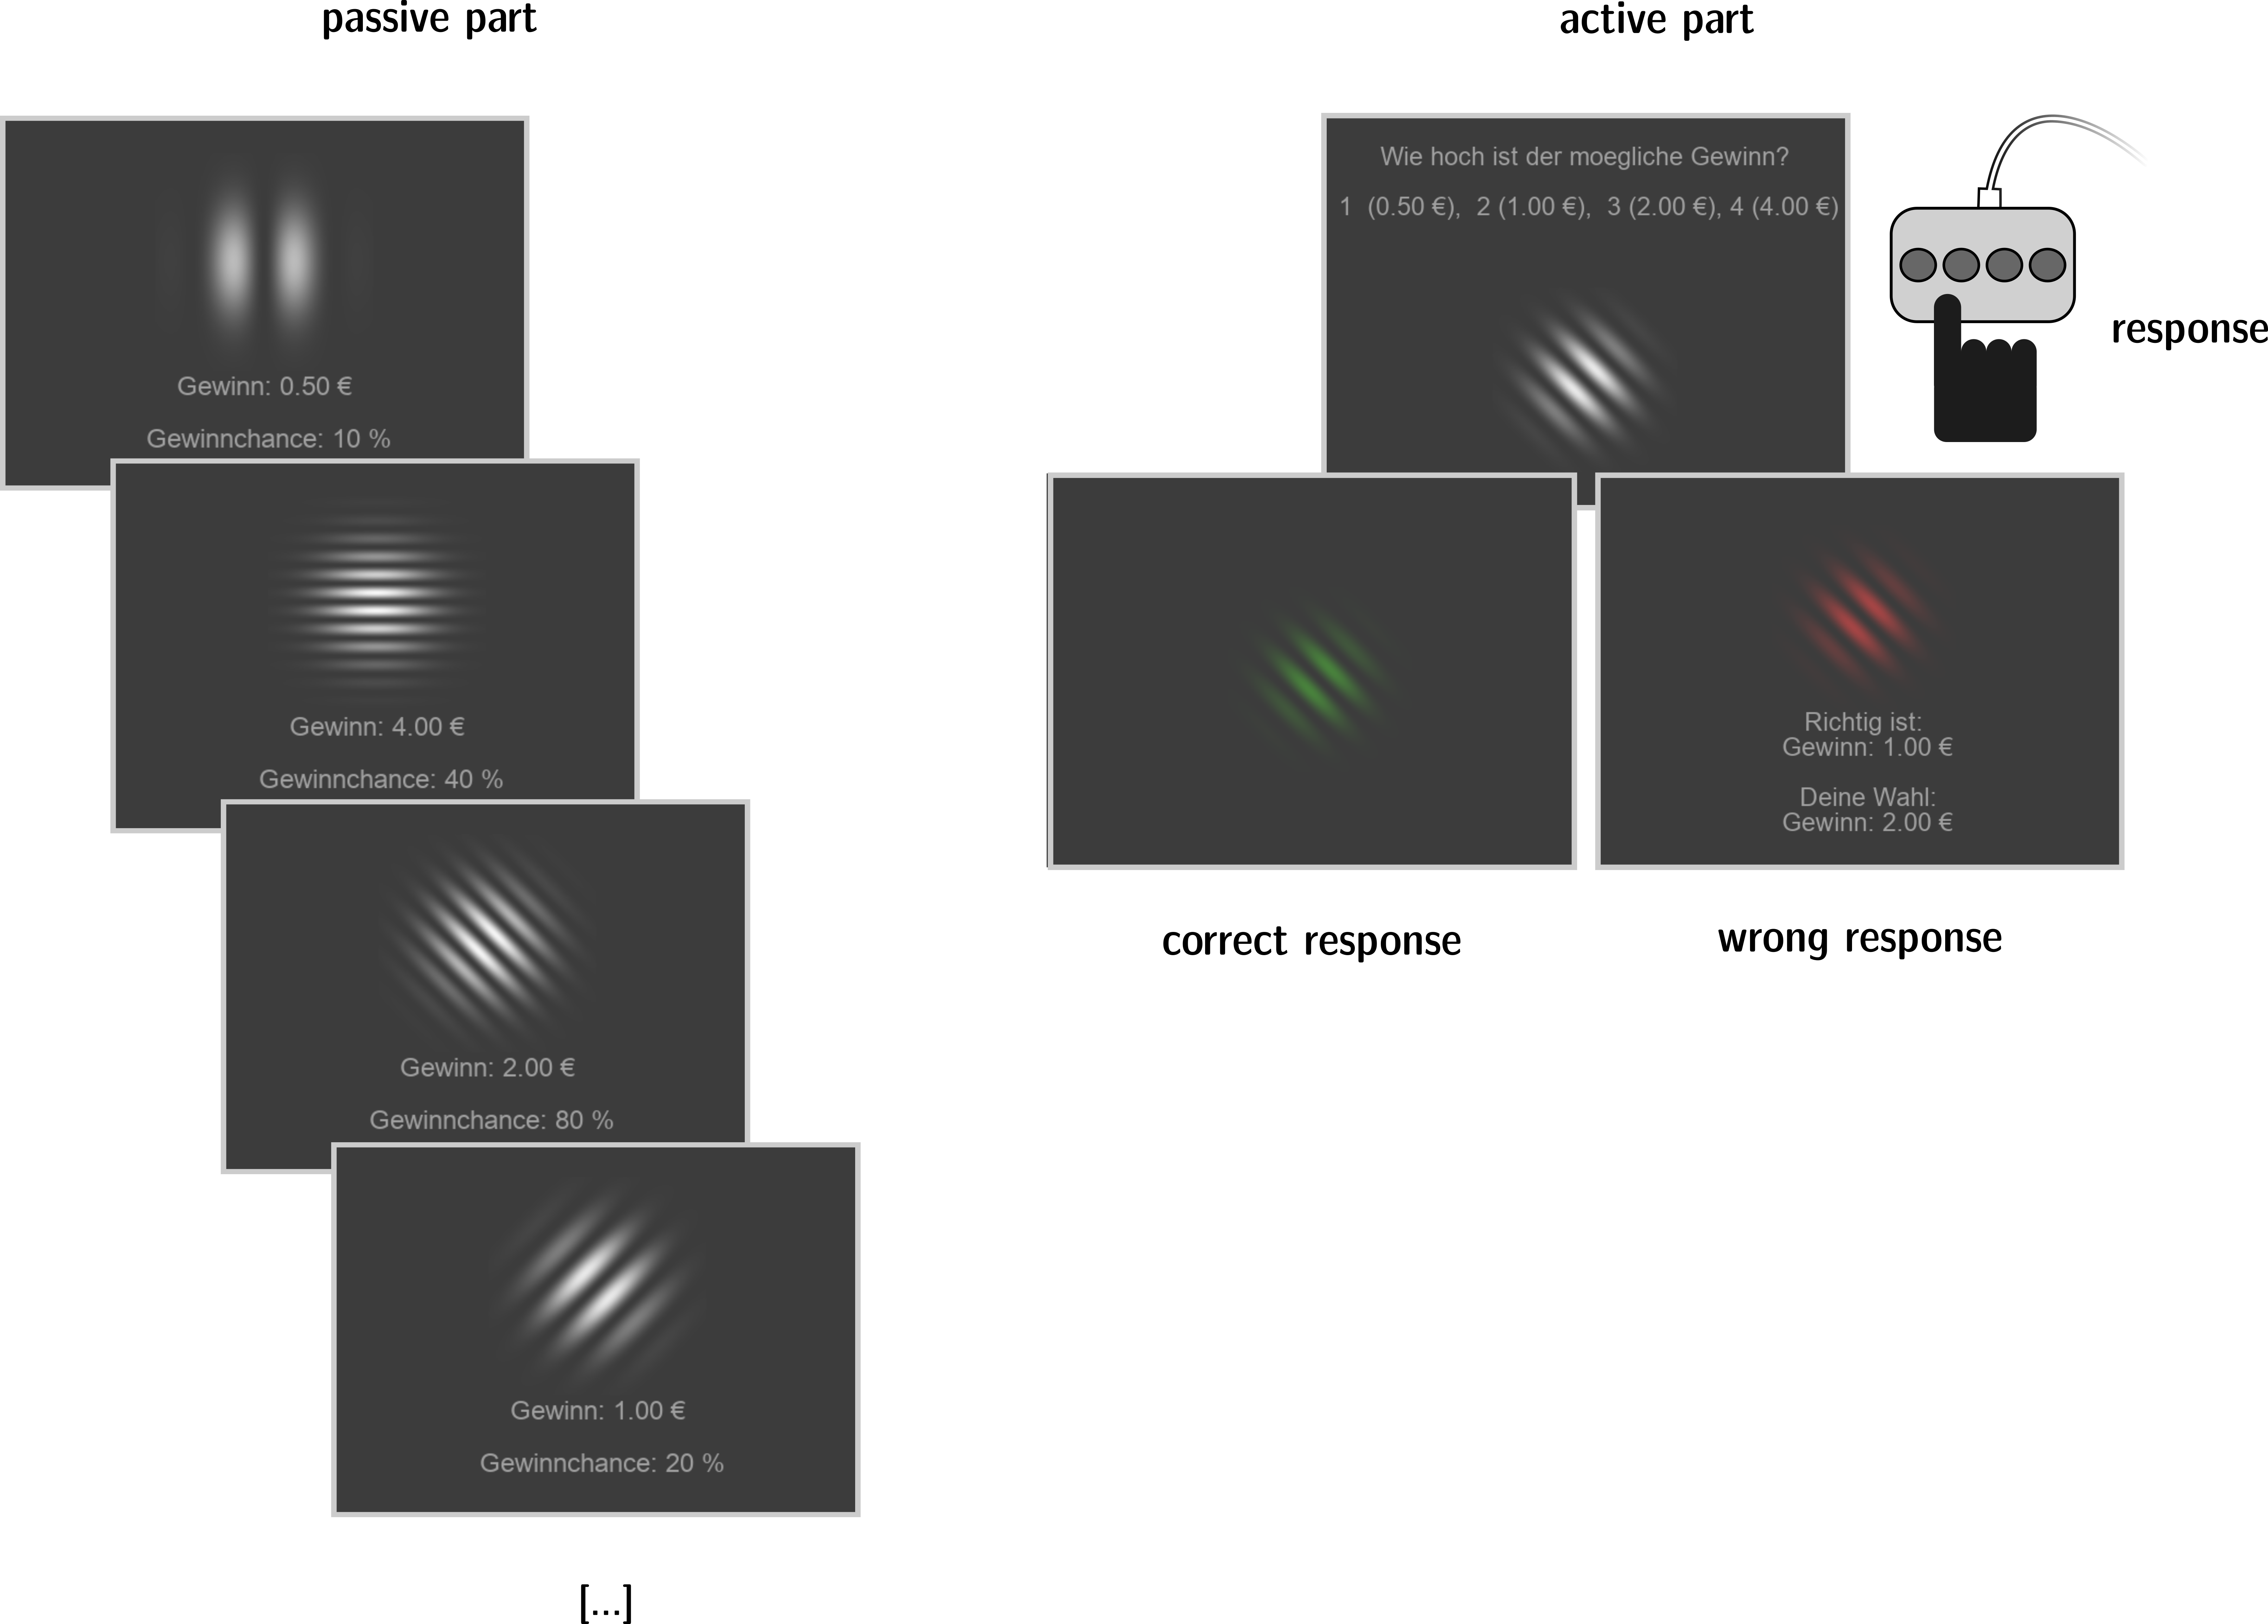
\includegraphics[width=\textwidth]{memento/memento_tutorial.png}
	\caption{Schematic overview of the tutorial.}
	\label{fig:memento_tutorial}
	\end{subfigure}
	\begin{subfigure}{.45\textwidth}
	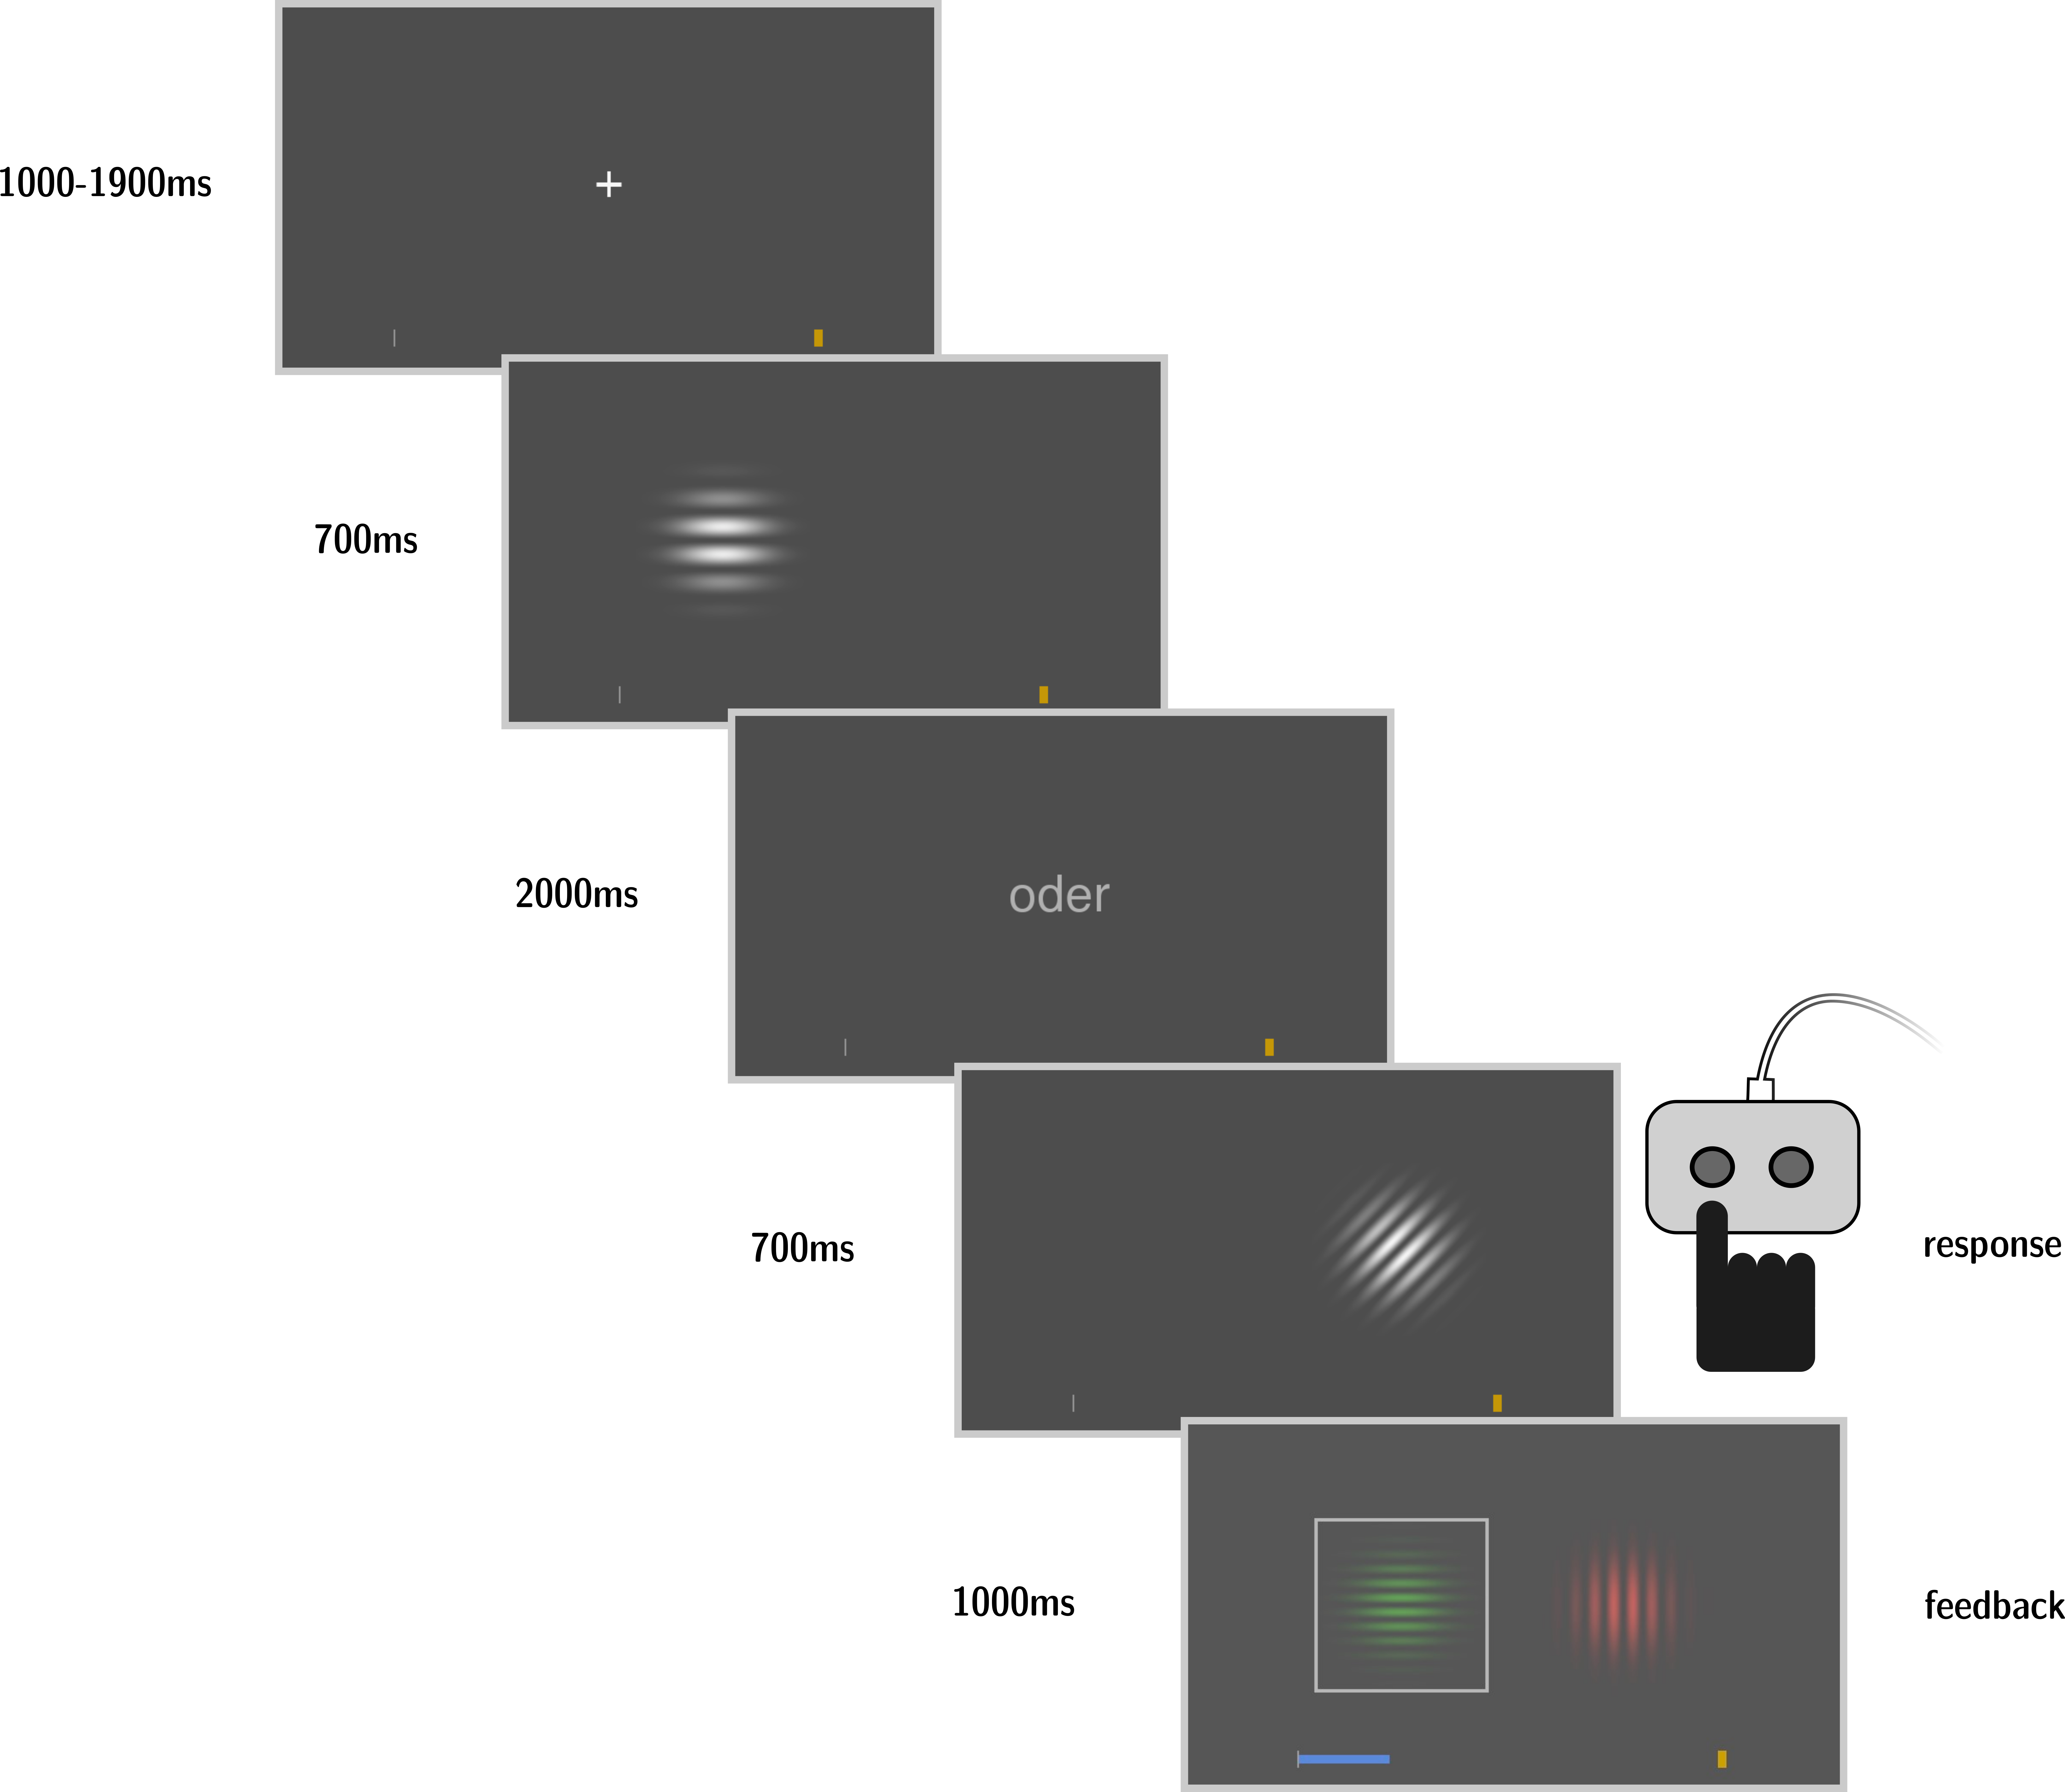
\includegraphics[width=\textwidth]{memento/memento_experiment.png}
	\caption{Schematic overview of a single trial.}
	\label{fig:memento_trial}
\end{subfigure}
	\caption[Memento: Tutorial and trial overview]{Schematic overview of the tutorial (\ref{fig:memento_tutorial}) and a single trial in the experiment (\ref{fig:memento_trial}).
	The tutorial was split in an active and a passive part.
	In the passive part, participants were presented with a stimulus and how its properties translated to reward magnitude and probability. All possible magnitude and probability combinations were presented twice, and participants controlled the pace. The active part then tested participants' knowledge by presenting a stimulus without the annotation. Based on a text prompt, participants had to report its associated magnitude or probability via button press. They received feedback with a green colored stimulus for a correct response, or, for an incorrect response, a red colored stimulus together with a report of their response versus the true response.
	}
\label{fig:memento}
\end{figure}


\subsection{MEG acquisition}

Following a metal test, MEG data were acquired on an Elekta Neuromag TRIUX System with internal helium recycler and 306 sensors (204 planar gradiometers and 102 magnetometers) in a magnetically shielded room.
Participants were instructed to take a comfortable seating position and sit as still as possible.
The experiment was presented on a screen in a distance of one meter from the sitting participants via a projector with a refresh rate of 60 Hz located outside the MEG recording chamber.
Additional sensors captured confounding biological signals:
Lateral and vertical eye movements and blinks were captured using electrooculography surface electrodes on the tori supra- and infraorbitalis and next to the external canthi.
Heartbeat artifacts were recorded with an electrocardiogram.
Head position indicator coils captured the participants head movements.
Behavioral responses were registered using an MEG compatible keyboard.
The neural data was recorded at a sampling rate of 1000Hz and active internal shielding (IAS).


\subsection{Preprocessing}

Prior to preprocessing, raw data were restructured to \gls{BIDS} format (v1.4.0) using mne-bids \citep{Appelhoff2019}.
Simultaneously, behavioral log files were transformed from proprietary .mat into the TSV format.

As the first step of preprocessing, the spatiotemporal extension of the \gls{SSS} method \citep{taulu2005presentation}, \textit{\gls{tSSS}} \citep{taulu2006spatiotemporal}, was applied, as is common for recordings on Neuromag MEG systems with active internal shielding.
\gls{SSS} and \gls{tSSS} remove strong interference from external noise sources and sources within the body itself from the MEG signal.
The methods can be applied on whole-scalp multichannel data when the precise sensor calibrations are known, and were initially developed as the proprietary MaxFilter\textsuperscript{TM} algorithm by Elekta Neuromag.
To this end, Neuromag systems provide a cross-talk compensation and fine calibration file which reduces interference between their co-located magnetometer and paired gradiometer sensor units and encodes site-specific information about sensor orientation and calibration, respectively.
Based on the Maxwell equations \citep{taulu2006spatiotemporal}, \gls{SSS} decomposes \gls{meg} signals ($\phi$) into elementary magnetic fields from sources within the sensor helmet (the \textit{internal} subspace) and into an orthogonal set for fields arising from sources outside (the \textit{external} subspace).

\begin{equation}
	\begin{aligned}
	  \phi = \sum_{l=1}^{\inf}\sum_{m=-l}^{l} \alpha_{lm} a_{lm} + \sum_{l=1}^{L_{out}}\sum_{m=-l}^{1}\beta_{lm}b_{lm}
	\end{aligned}
\label{eq:sss}
\end{equation}

Based on this, it transforms the $N=306$-dimensional signal vector into a lower dimensional subspace that spans all measurable signals, the ``SSS basis'' $S$. Its subspaces $S_in$ and $S_out$ contain the biomagnetic signal and arbitrary external interference, respectively.

\begin{equation}
	\begin{aligned}
		    \phi &= S_x = [S_{in} S_{out}] \begin{bmatrix}
			x_{in} \\
			x_{out}
		\end{bmatrix}
	\end{aligned}
	\label{eq:sss}
\end{equation}

The SSS basis is $n=(L_{in}+1)^2+(L_{out}+1)^2$-dimensional, with typical model orders $L_{in}=8$ and $L_{out}=3$, resulting in $n=95$ (80 internal, 15 external) dimensions.
With $n \ll N$, $\phi$ can be uniquely decomposed into internal and external components

\begin{equation}
	\begin{aligned}
			\phi &= S_x = [S_{in} S_{out}] \begin{bmatrix}
			x_{in} \\
			x_{out}
		\end{bmatrix} = \phi_{in} + \phi_{out}
	\end{aligned}
	\label{eq:sss}
\end{equation}

As the internal and external subspaces are provably linearly independent, brain signals are then reconstructed by retaining only sources inside the helmet, thus excluding external inferences.


\begin{equation}
	\begin{aligned}
    \hat{x} =
\begin{bmatrix}
	\hat{x}_{in} \\
	\hat{x}_{out}
\end{bmatrix}
= S^{\dagger}\phi \\
\hat{\phi}_{in} = S_{in}\hat{x}_{in}\\
	\end{aligned}
	\label{eq:sss}
\end{equation}


According to \citet{taulu2006spatiotemporal}, \gls{SSS} can separate brain signals from sources >0.5m away, suppressing external interference by a factor >100.
The spatiotemporal extension \gls{tSSS} can further detect inferences from closer sources such as stimulators or pacemakers.
These are estimated based on the fact that their strength typically exceeds that of sensor noise and they thus, unlike brain signal, leak into both the internal and external part of the \gls{SSS} reconstruction.
After detecting components with a high temporal correlation between the external and internal subspaces, \gls{tSSS} removes close-by artifacts by projecting the components common to the internal and external subspace out of the internal subspace.
In the absence of nearby artifacts, \gls{tSSS} reduces to \gls{SSS} \citep{taulu2009removal}.
\gls{tSSS} was implemented using mne-python's open source implementation \texttt{maxwell\_filter()} with a chunk duration of 10 seconds and a correlation threshold of at least $0.98$.
Prior to \gls{tSSS}, bad channels were detected and annotated automatically in order to prevent bad channel noise from spreading.
To compensate for head movements, measurements from the head position indicator coils were used to estimate subject motion, and motion correction was then performed as part of the \gls{tSSS} procedure: As the signal representation in the \gls{SSS} basis is device independent, internal data can simply be transformed to a sensor array corresponding to the average head position.
After \gls{tSSS}, gradiometers and magnetometers contain highly similar information and have an altered inter-channel correlation structure because they were reconstructed from a common 80-dimensional subspace \citep{jas2018reproducible}.
Formerly bad channels have also been effectively repaired by the procedure.
After \gls{tSSS}, some spectral artifacts remained in the data, among them power line noise at 50Hz and a spectral peak at 60Hz, likely originating from the presentation screen's refresh rate.
ZAPline filtering \citep{de2020zapline} was performed to remove them using \texttt{meegkit} \citep{barascud2022}.
Figures \ref{fig:prezap} and \ref{fig:postzap} show power spectral density plots of the signal pre and post (effective window size: 2.048 s) applying ZAPline filters.


\begin{figure}
	\begin{subfigure}{.49\textwidth}
		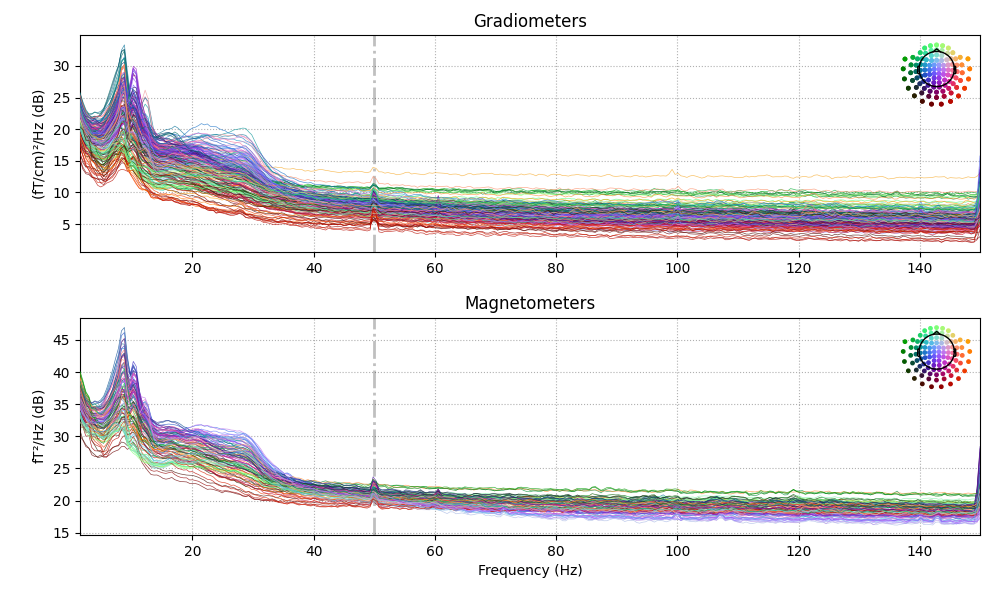
\includegraphics[width=\textwidth]{memento/psd_pre_zapline.png}
		\caption{Power spectral density before ZAPline filtering}
		\label{fig:prezap}
	\end{subfigure}
	\begin{subfigure}{.49\textwidth}
		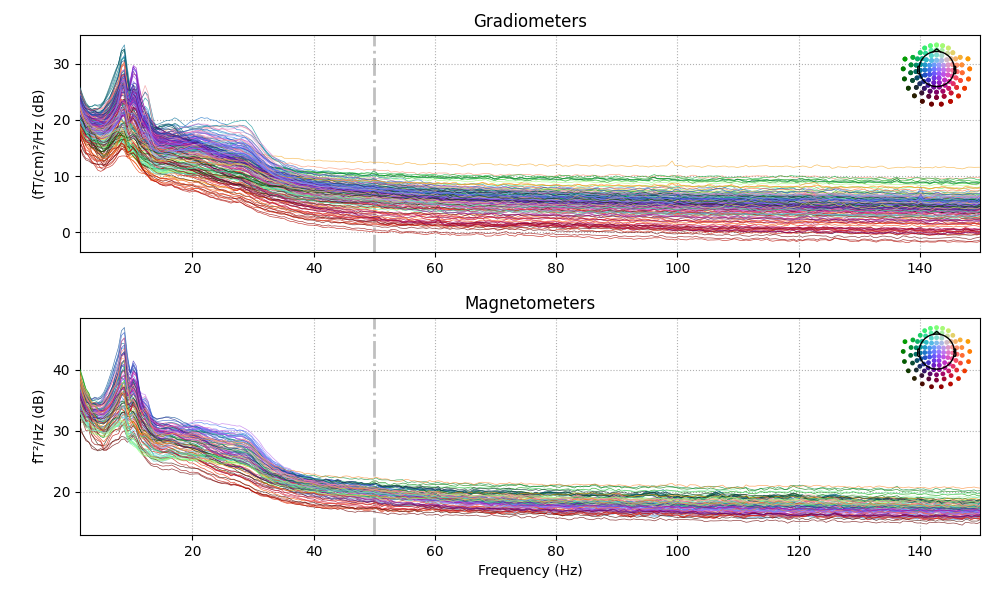
\includegraphics[width=\textwidth]{memento/psd_post_zapline.png}
		\caption{Power spectral density after ZAPline filtering}
		\label{fig:postzap}
	\end{subfigure}
	\caption[Power spectral density before and after ZAPLine filtering]{Power spectral density of all MEG channels
		from a single subject before (\ref{fig:prezap}) and after (\ref{fig:postzap}) ZAPLine filtering.
		Two spikes at 50Hz (power-line frequency) and 60Hz (likely an artifact of the stimulus presentation) are markedly reduced afterwards.
	}
	\label{fig:zapline_psd}
\end{figure}

Next, data were first low-pass filtered with a 100Hz lowpass FIR filter to constrain it into a frequency range of interest.
The filter properties are reported in \ref{fig:preproc} and a visualization is in \ref{fig:filter}.
As eye movements, eye blinks, heart beats, and facial muscle contractions survive \gls{tSSS}, \gls{ica} was used to detect and remove these artifacts.
% The slow drifts are problematic because they reduce the independence of the assumed-to-be-independent sources (e.g., during a slow upward drift, the neural, heartbeat, blink, and other muscular sources will all tend to have higher values), making it harder for the algorithm to find an accurate solution. A high-pass filter with 1 Hz cutoff frequency is recommended. However, because filtering is a linear operation, the ICA solution found from the filtered signal can be applied to the unfiltered signal https://ieeexplore.ieee.org/document/7319296/
As ICA is sensitive to low-frequency drifts \citep{winkler2015ICA}, the data were first processed with a temporary one-pass, zero-phase, non-causal highpass filter (firwin method, Hamming window with 0.0194 passband ripple and 53 dB stopband attenuation, a lower passband edge of 1.00, lower transition bandwidth of 1.00 Hz (-6 dB cutoff frequency: 0.50 Hz), and a filter length of 3301 samples (3.301 s)).
As ICA can further be sensitive to bad segments in the recording, data were temporarily epoched into 5 second splits from the onset of the fixation cross.
\texttt{autoreject} was then used on the first 200 of these epochs to estimate the noise level and compute rejection thresholds.
Afterwards, FastICA \citep{hyvarinen1999fast} was used to decompose the signal into 45 independent components.
For most subjects, components corresponding to ECG activity were identified using cross-trial phase statistics \citep{dammers2008integration} with an automatically computed threshold of 0.16 for the Kuiper statistic, and EOG related components were found using Pearson correlation.
For one subject, however, the ECG channel was flat, and components were manually selected.
Afterwards, the ICA solution was applied to the continuous recording and detected ECG and EOG components were zeroed out.

As a final step, the continous recording was chunked into Epochs of varying length depending on analysis, and \texttt{autoreject} was used to detect and repair or drop bad epochs.
Figure \ref{fig:preproc} summarizes the preprocessing steps.
Figure \ref{fig:cleanepoch} shows an average of cleaned 5 second epochs for a single subject.



\begin{figure}
	\begin{subfigure}{0.4\textwidth}
		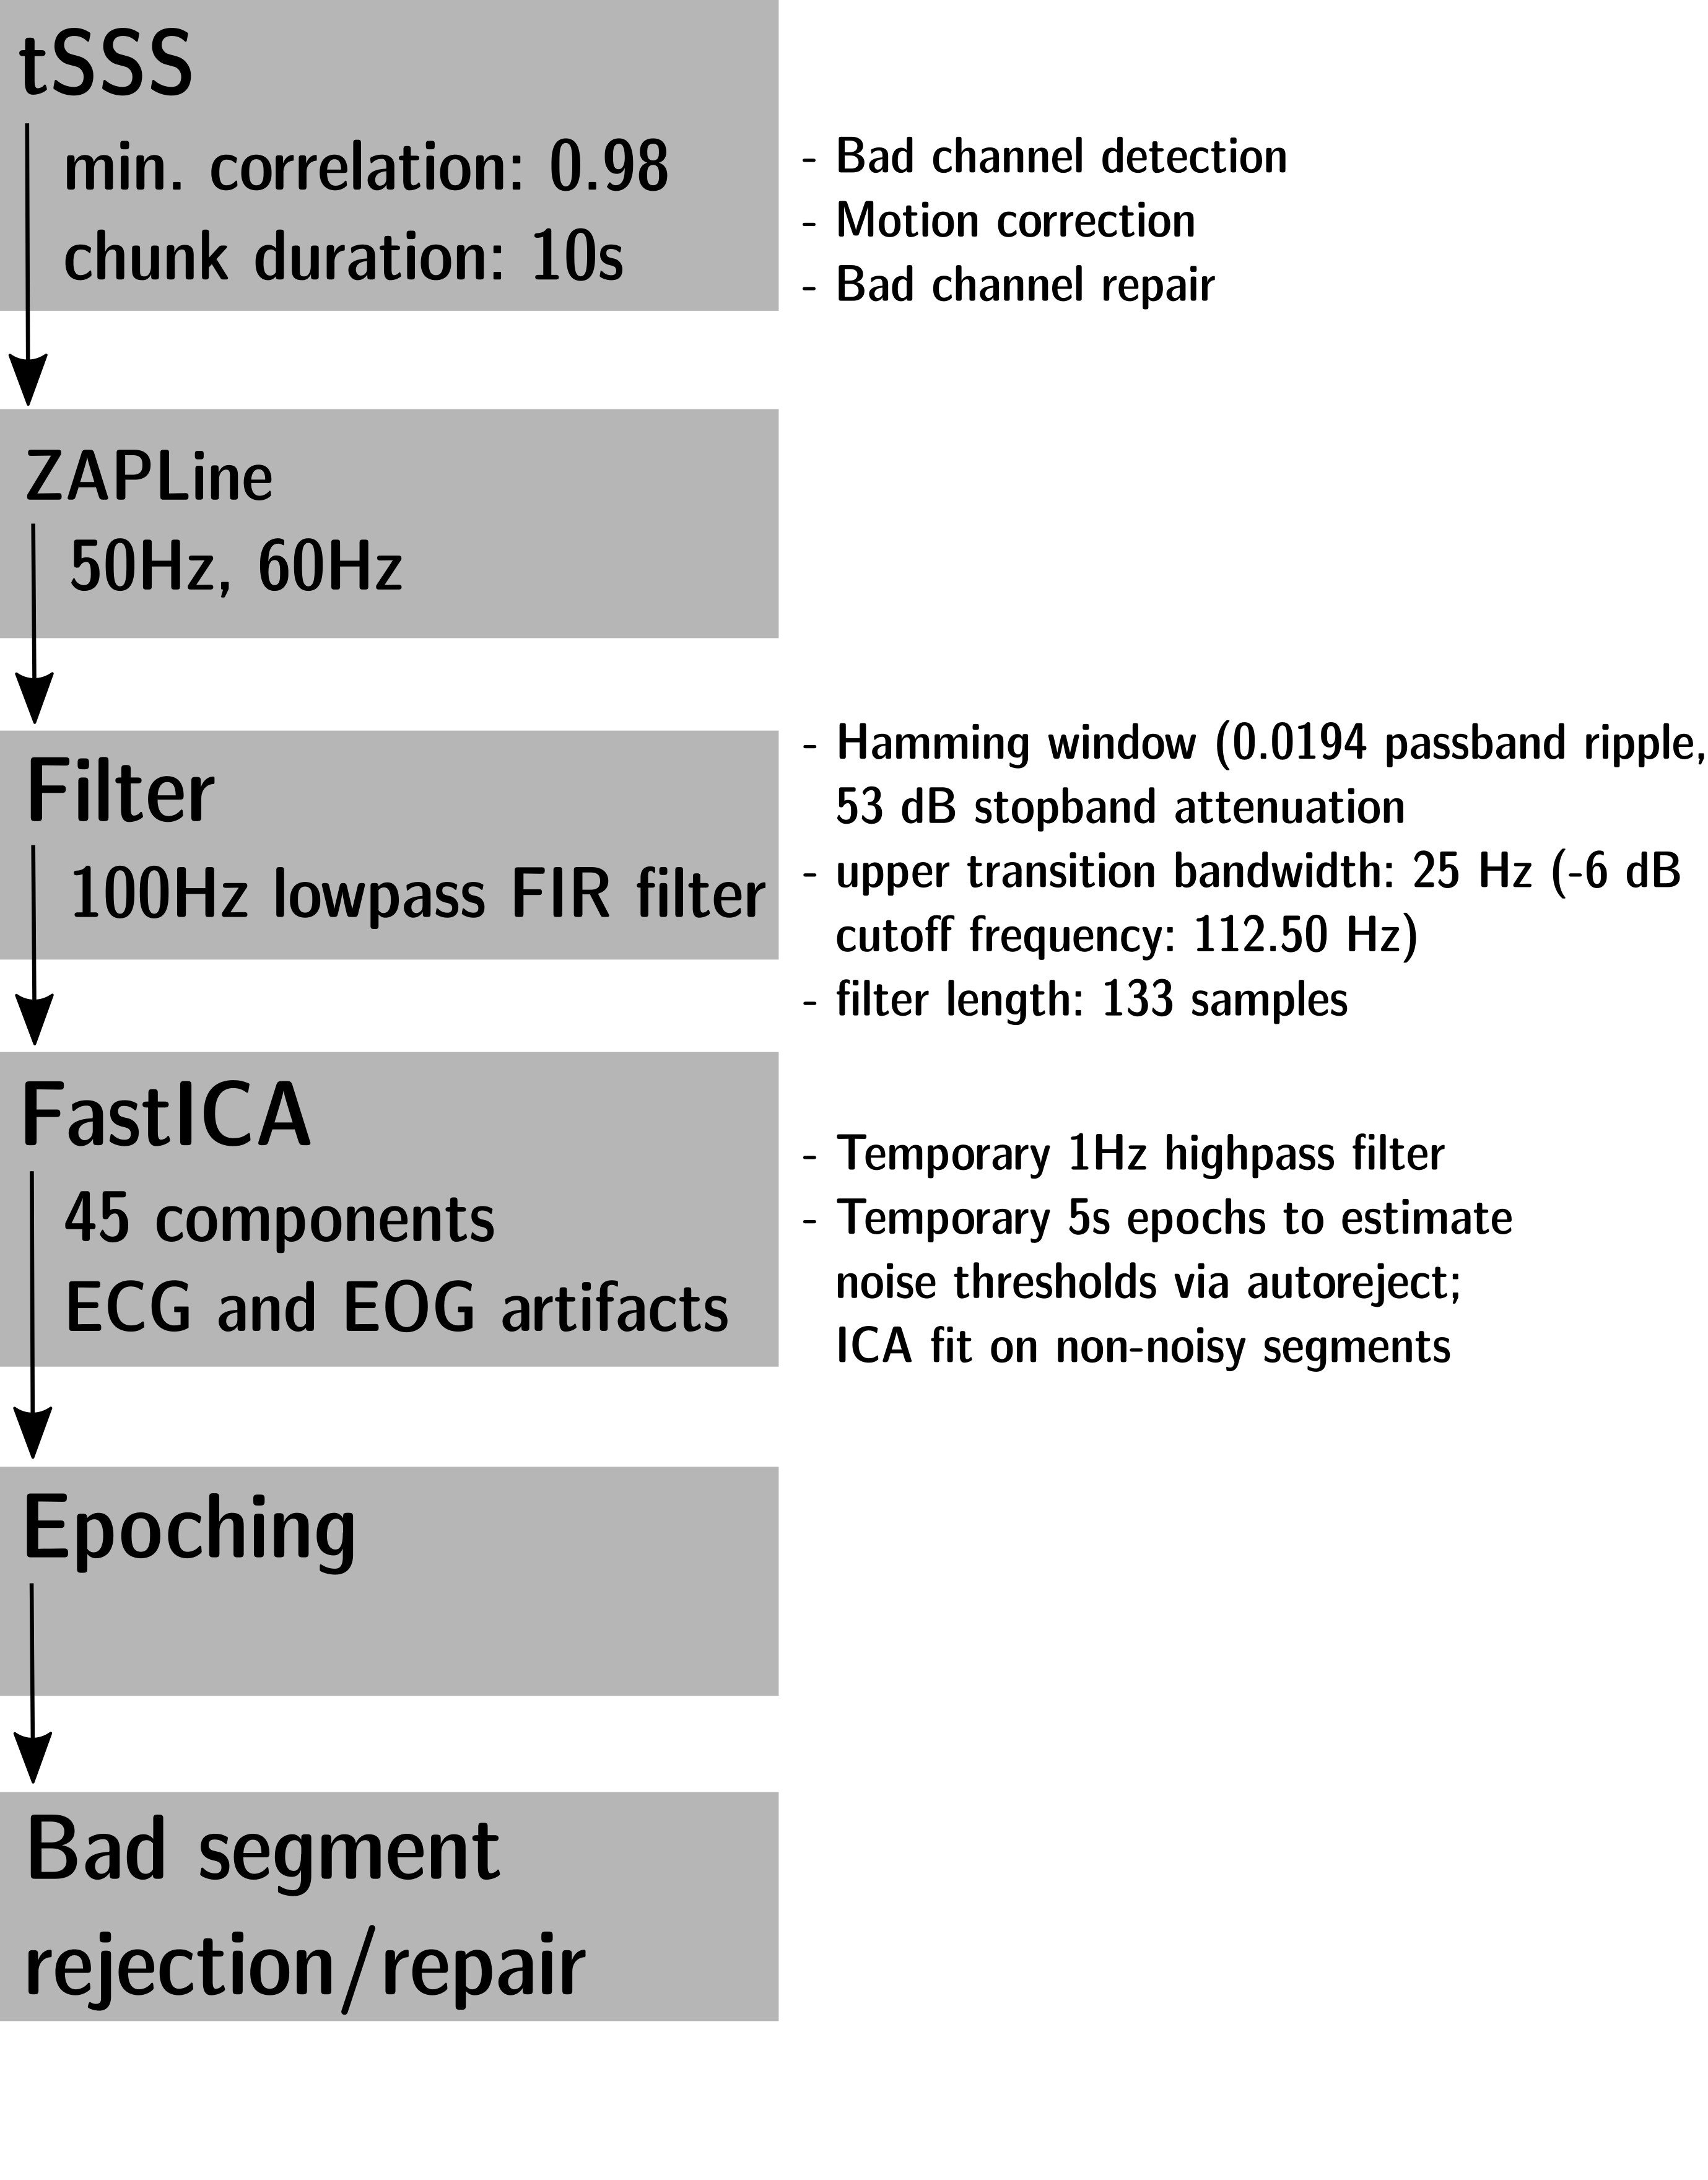
\includegraphics[width=\textwidth]{memento/preprocessing_overview.png}
		\caption[Preprocessing overview]{Preprocessing Overview}
		\label{fig:preproc}
	\end{subfigure}
	\begin{subfigure}{0.4\textwidth}
		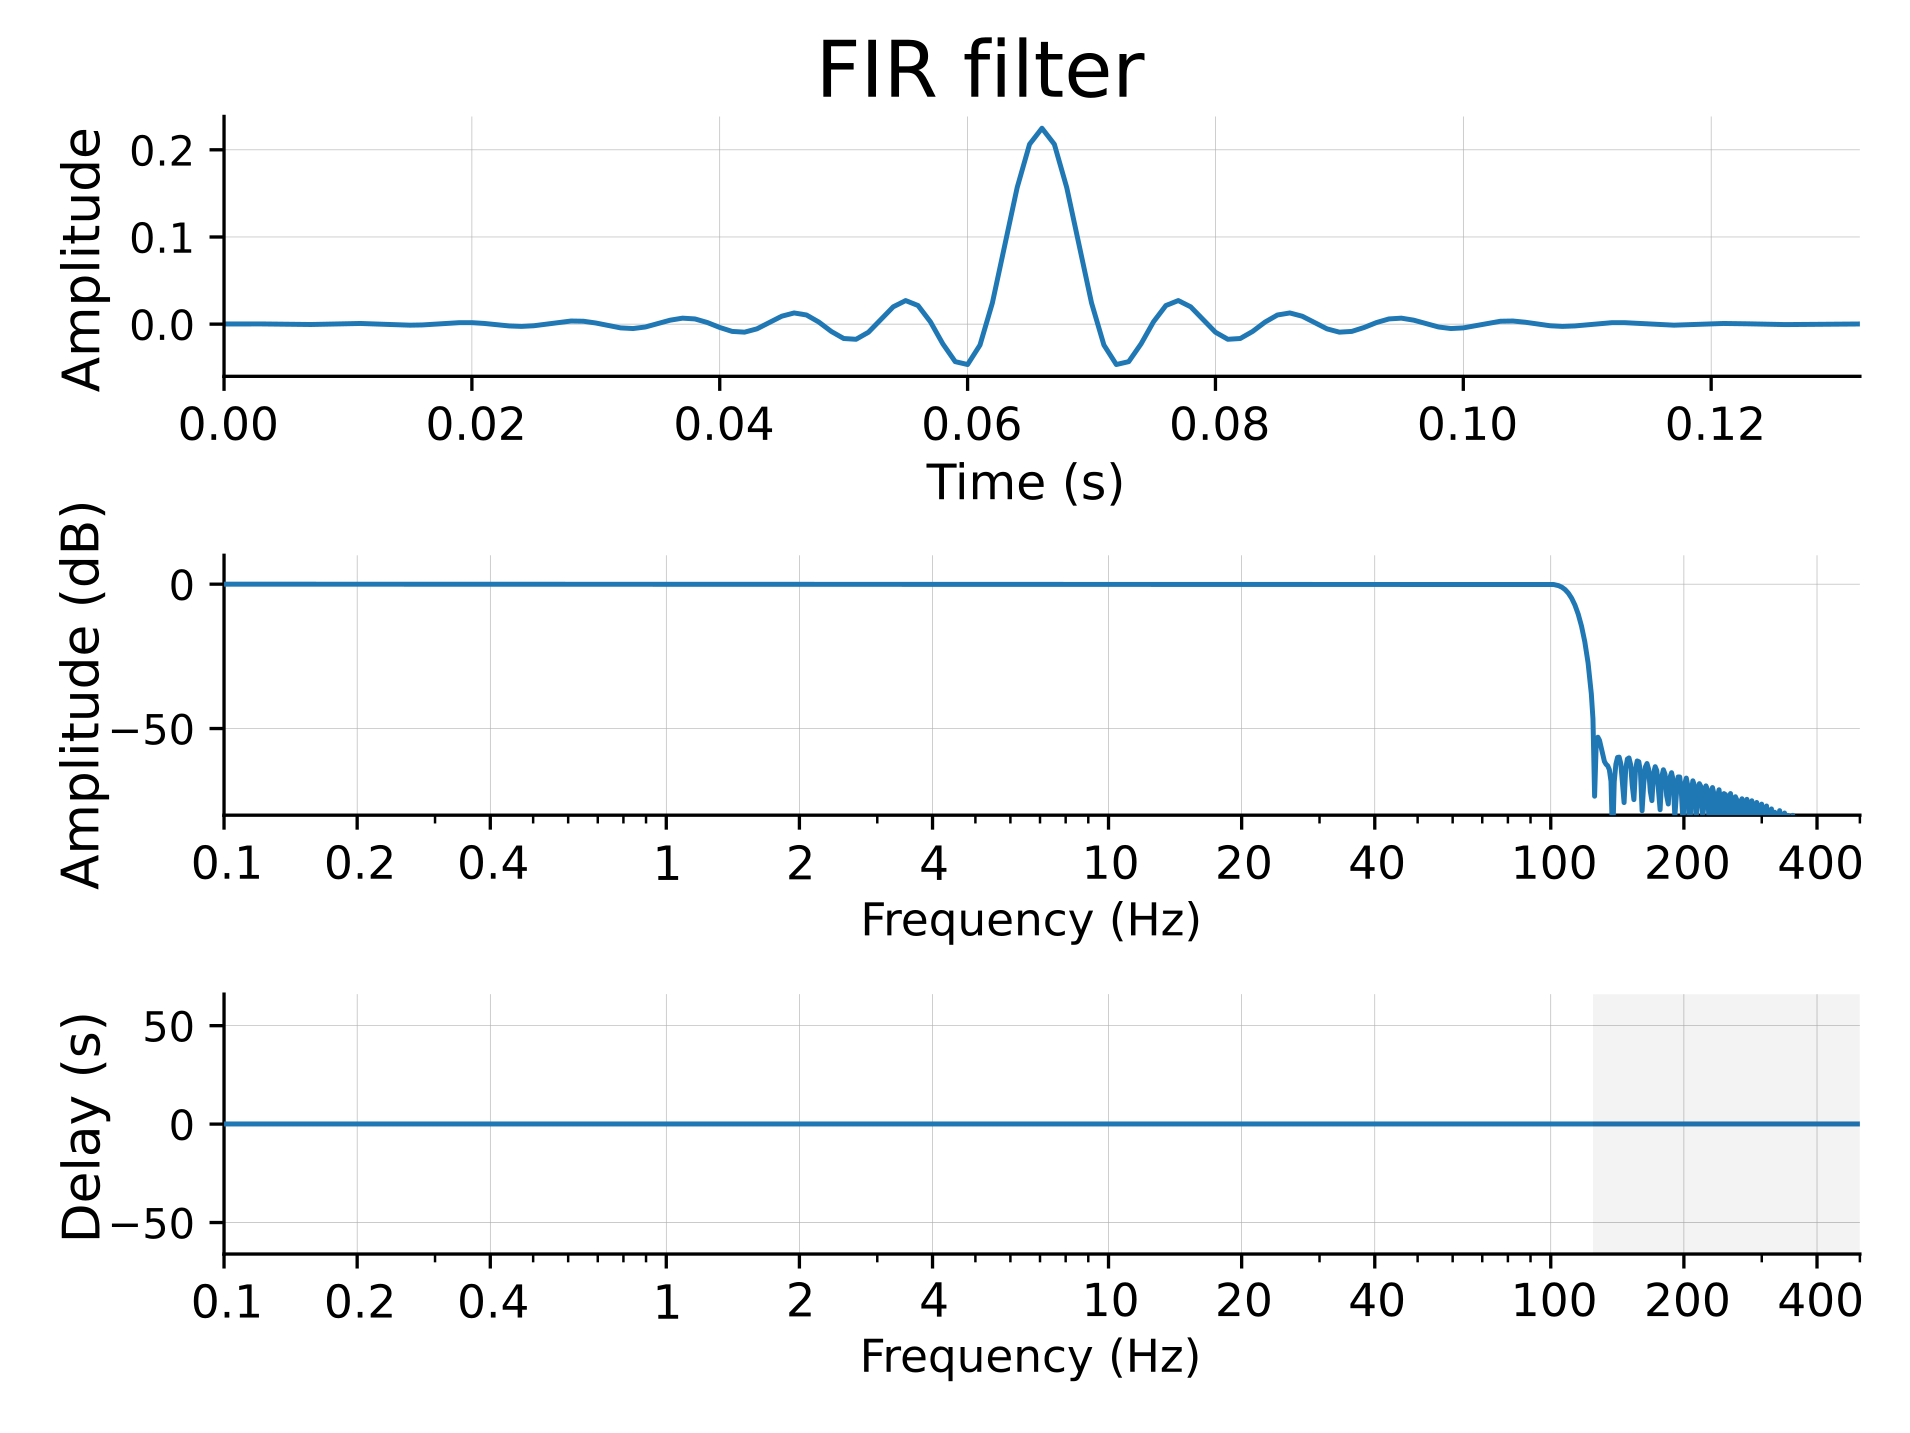
\includegraphics[width=\textwidth]{memento/filter_properties_100hz.png}
		\caption[Lowpass filter properties]{Lowpass filter properties}
		\label{fig:filter}
	\end{subfigure}
	\caption[Preprocessing]{Preprocessing thingies}
\end{figure}

\begin{figure}
	\centering
	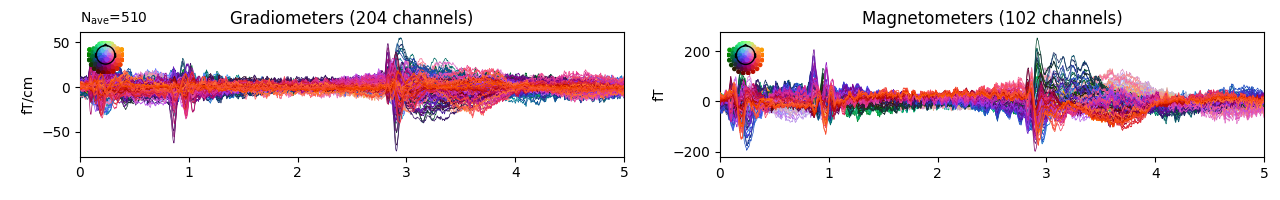
\includegraphics[width=0.5\textwidth]{memento/average_epoch_cleaned.png}
	\caption[Average neural signal over the trial course]{Neural recordings from a single exemplary subject.
		Shown is the average of cleaned epochs with a length of 5 seconds from left stimulus onset, corresponding to a trial from first visual stimulation until
		1600ms after the offset of the second stimulus.}
	\label{fig:cleanepoch}
\end{figure}

All preprocessing steps and the subsequent analysis were implemented using mne python (CITE) or custom Python functions. All preprocessing and analysis scripts are openly available on GitHub and as the python package \texttt{pymento\_meg} (CITE).


\pagebreak

\section{Shared response modeling}

% This needs a general introduction into shared response modeling
The underlying assumption of functional alignment methods is that brain activity can be modeled in an n-dimensional space, where n is the number of measurements (e.g., voxels in \gls{fMRI}, sensors in \gls{meg}, or electrodes in \gls{eeg} acquisitions).
When subjects experience the same events, their brain activity may differ anatomically, but should correspond to similar cognitive processes.
To functionally align the brain activity of multiple participants, we align the vector representations of their brain signals.
Afterwards, we need to assign meaning to the axes of the shared space.

During \gls{tSSS}, the neural signal is decomposed from the 306 dimensional sensor space into an 80-dimensional subspace, the \gls{SSS} basis.
This confirms that the signal of interest can be expressed in fewer than 306 dimensions.
We therefore sought to find out whether we can find meaningful low-dimensional structure in the high-dimensional dataset via \gls{SRM} \citep{NIPS2015_b3967a0e}.

In \gls{SRM}, the objective is to model each subject $i$'s response to temporally synchronized stimuli as a subject-specific base $W_i$ and a shared component over all subject's responses $S$.
In an \gls{meg} acquisition, each subject $i$ has a data matrix of dimensions sensors $\times$ time-points.


\begin{equation}
	\begin{aligned}
    X_i \in \mathbb{R}^{s \times d}
	\end{aligned}
	\label{eq:sss}
\end{equation}

\gls{SRM} estimates a $k$-dimensional shared space $S$, and orthogonal-column basis vectors of the shared response in subject-space  $\{W_i\}^m_{i=1}$  $\{W_i\}^m_{i=1}$


\begin{equation}
	\begin{aligned}
	    min_{w_i, s}\sum_i{\|X_i - W_iS \|}^2_F \\
	s.t. W^T_iW_i = I_k
	\end{aligned}
	\label{eq:sss}
\end{equation}


\begin{figure}
	\centering
	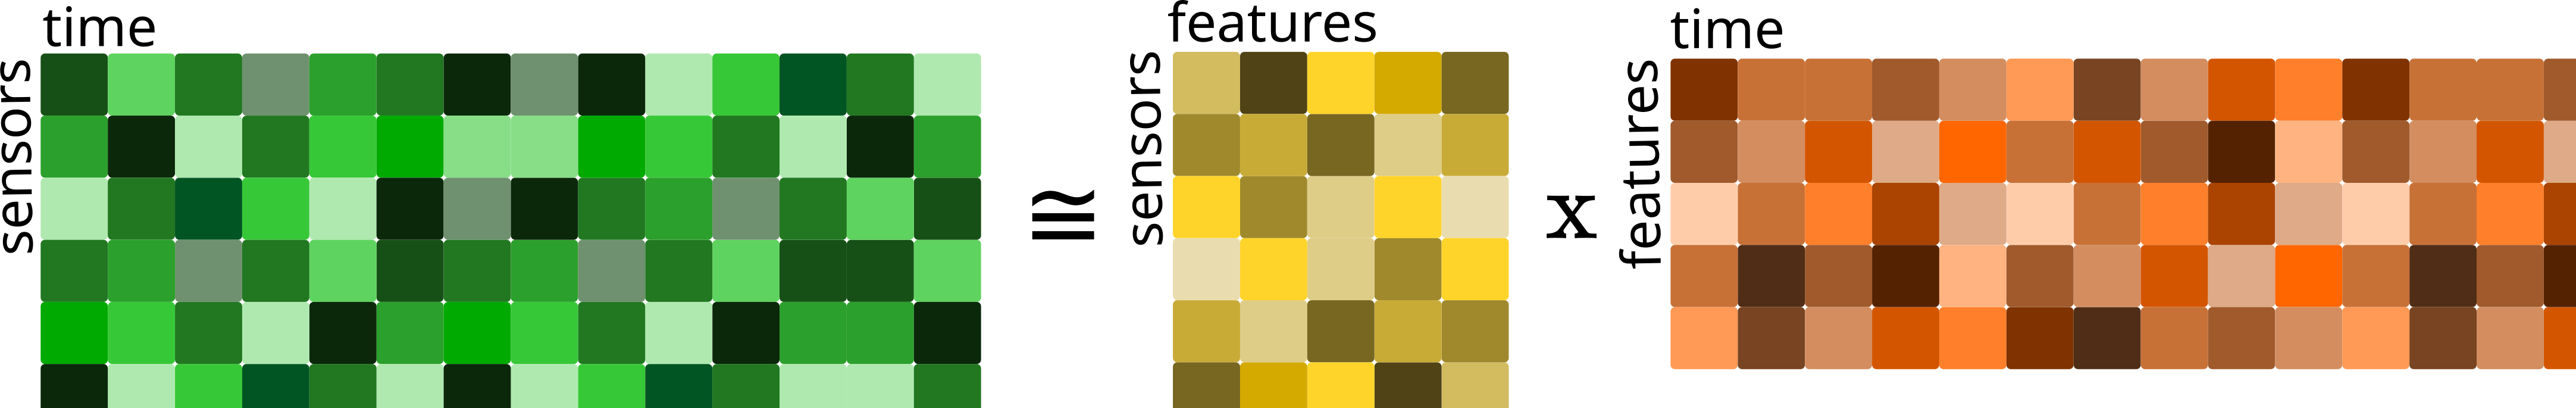
\includegraphics[width=0.9\textwidth]{memento/srm/srm_basics_1.png}
	\caption[SRM overview]{In \gls{SRM} on \gls{meg} data, sensor-by-time matrices are decomposed into a orthogonal subject specific basis matrix (sensor-by-features), a common shared feature matrix (features-by-time), and a subject-specific error}
	\label{fig:srm-basics}
\end{figure}

Given participants experience the same sequence of stimulus events, \gls{SRM} identifies common activity patterns across subjects, and provides a method to transform the original activity into a lower dimensional shared latent component space.
Where the original data in sensor space is a $306$ sensors $\times$ number of samples matrix, the shared response space is a $k$ features $\times$ number of samples matrix.


\begin{figure}
	\centering
	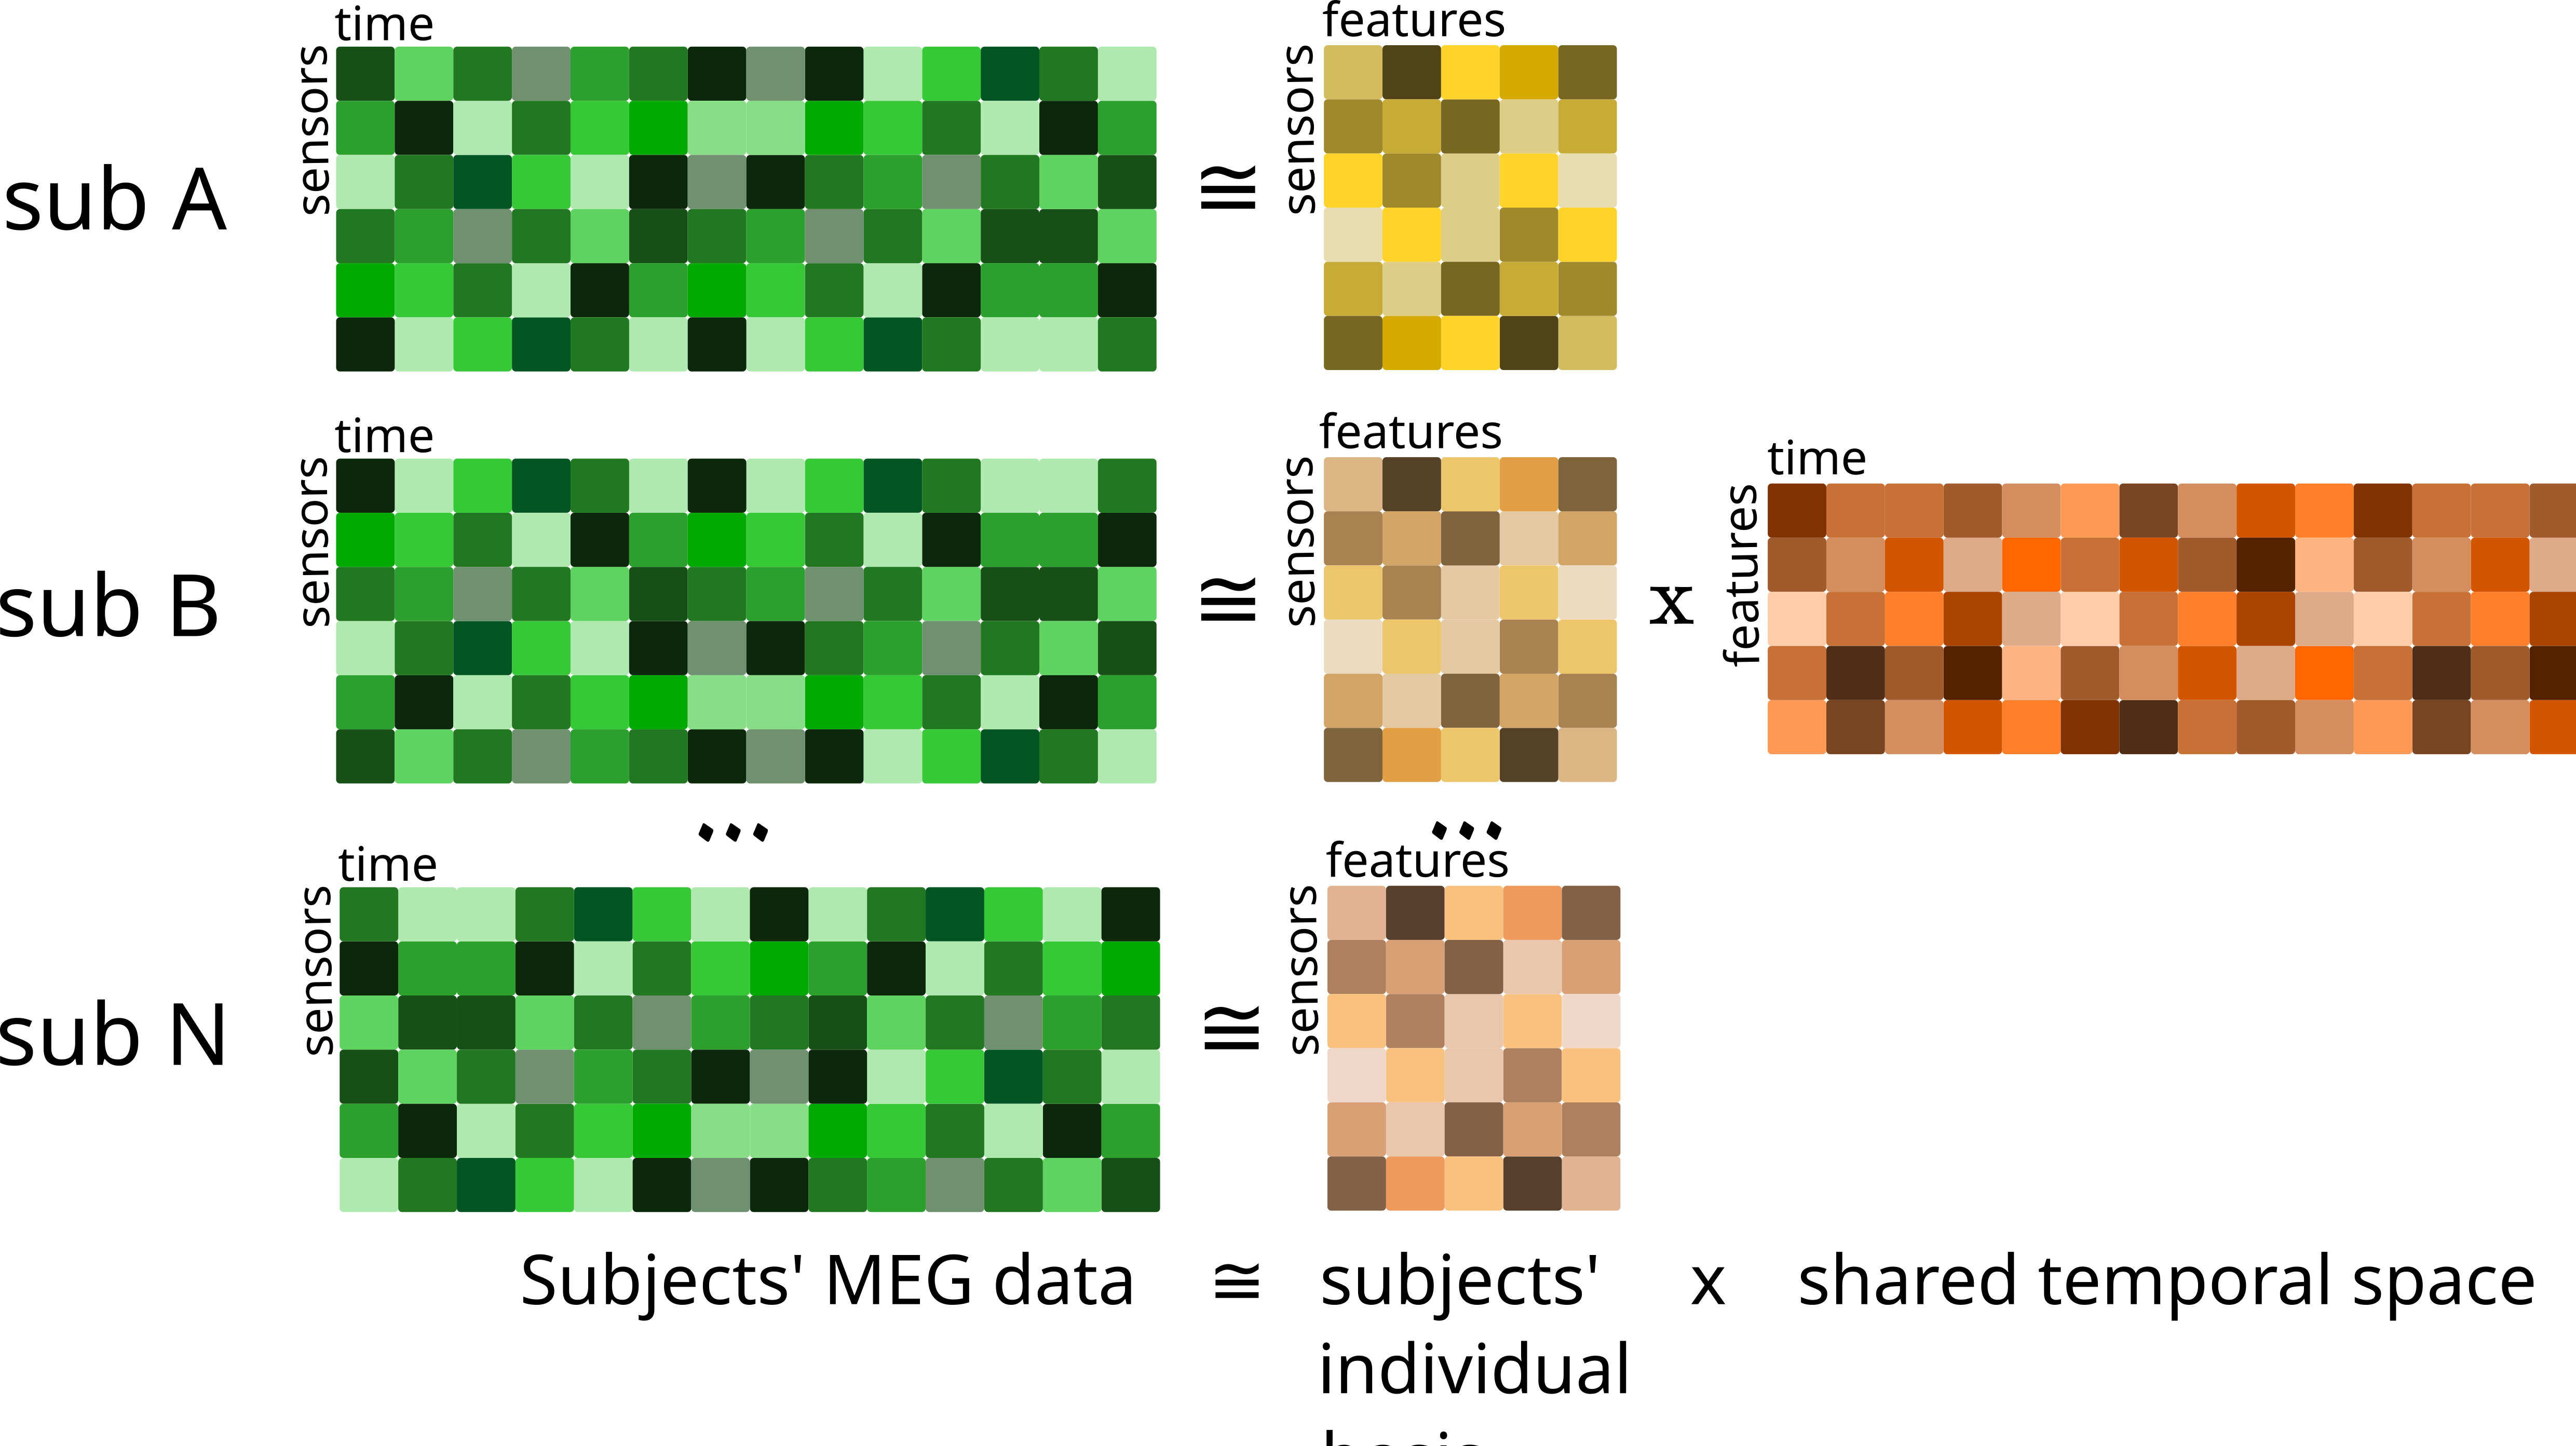
\includegraphics[width=0.9\textwidth]{memento/srm/srm_basics_3.png}
	\caption[SRM overview]{SRM overview: Sensor-by-time matrices are decomposed into a orthogonal subject specific basis matrix (sensor-by-features), a common shared feature matrix (features-by-time), and a subject-specific error}
	\label{fig:srm-basics-multi}
\end{figure}

\gls{SRM} has only few assumptions: %list assumptions here
One important assumption is, though, that participants experience the same sequence of stimulus events.
To meet this assumption, epochs from the experiment were brought into a standardized order (CITE CHEN PRESENTATION)
% to do: probabilistic shared response modeling

\subsubsection{Sanity checks}

While \gls{SRM} is successfully and widely used with fMRI data (cite Elizabeth), in particular for naturalistic acquisitions with free-viewing tasks and movie stimuli (cite Sam), the method is only rarely used in \gls{meg}.
Thus the methods' utilities was first tested with a number of analyses intended to serve as sanity checks.




I first sanity checked whether basic stimulus properties are retained in the lower-dimensional shared response space of the model.
For this, I leveraged the nine different probability and magnitude combinations that were used for the left stimulus option (letters A-I in Figure \ref{fig:memento_stim}).
An underlying assumption for this is that neural signals differ across stimulus types.

Regardless of whether MEG data in sensor space


% trial ordering

We normalized epoch data by z-scoring each epoch within sensors.
For this, a shared response model was trained on a subset of data.
Next, we calculated the correlation distance between the shared response during one type of trial to al other trial types, for both the left and the right stimulus option.


\section{Shared response modeling in spectral space}

MEG signal consists of oscillations with an amplitude, a frequency, and a phase.
Frequency, usually measured in hertz (Hz), is the number of times a specified event occurs within a specified time interval, while amplitude is the height, force or power of the wave, and power is the squared amplitude.
Phase involves the relationship between two or more signals that share the same frequency and describes the relationship between the position of the amplitude crests and troughs of two waveforms, measured in distance, time, or degrees.
If the peaks of two signals with the same frequency are in exact alignment at the same time, they are said to be in phase.
Conversely, if the peaks of two signals with the same frequency are not in exact alignment at the same time, they are said to be out of phase.
While shared response modeling, just like similar methods of hyper alignment [CITE], relies on the assumption that different participants display similar cognitive processes in response to the same tasks or stimuli [CITE], the exact timing or duration of such shared activity is subject to intra- and interindividual variation, and thus not necessarily phase-locked. [CITE]
[Link this to decision making tasks and previous methodological developments, such as Hidden Markov Models]

Spectral analysis consists of deconstructing a time domain signal of a given length into its constituent oscillatory components using Fourier analysis.
The resulting power spectrum displays a spectral decomposition, with the frequency domain of the oscillations on the x axis, and the amplitude on the y axis.
Thus, the signal is expressed as a function of frequency rather than time.
Such a transformation from a time-resolved representation of data to a representation in the frequency domain can be used to find shared signals with different temporal signatures [CITE probably every introductory MEG book].
Importantly, the model bases of an \gls{SRM} assign weights to sensors regardless of whether they contribute to a shared signal in time-resolved or spectral space.
Therefore, we can fit a shared response model on spectral data to find shared frequency components, but then use the model basis to transform time-resolved data (see Figure \ref{fig:spectral-srm}).
This not only allows the visualization of shared components as a time series, but also easier interpretation of components in the context of the experimental paradigm.


\begin{figure}
	\centering
	\begin{subfigure}{0.9\textwidth}
		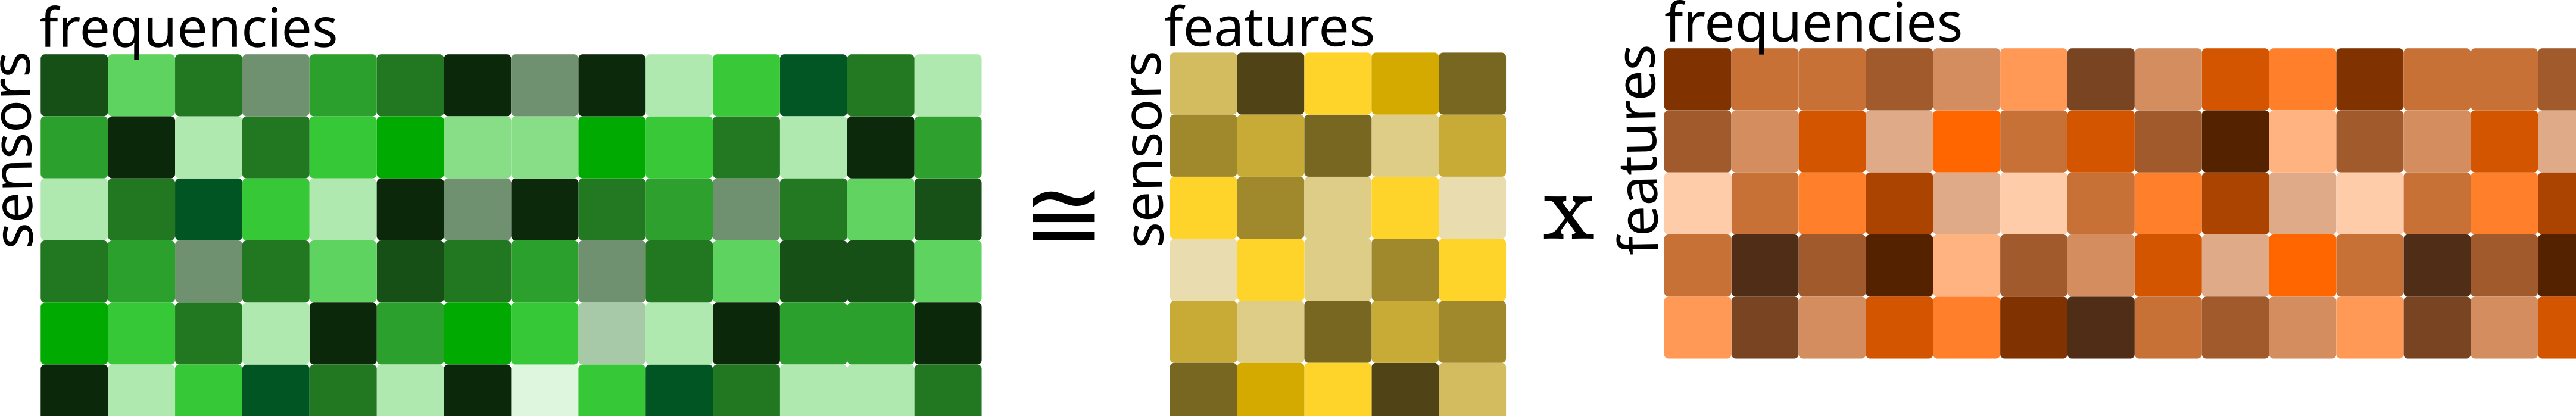
\includegraphics[width=\textwidth]{memento/spectral_srm/spectral_srm_basics_1.png}
		\caption{Fitting the shared response model on spectral data}
		\label{fig:spectral-srm1}
	\end{subfigure}
	\begin{subfigure}{0.9\textwidth}
		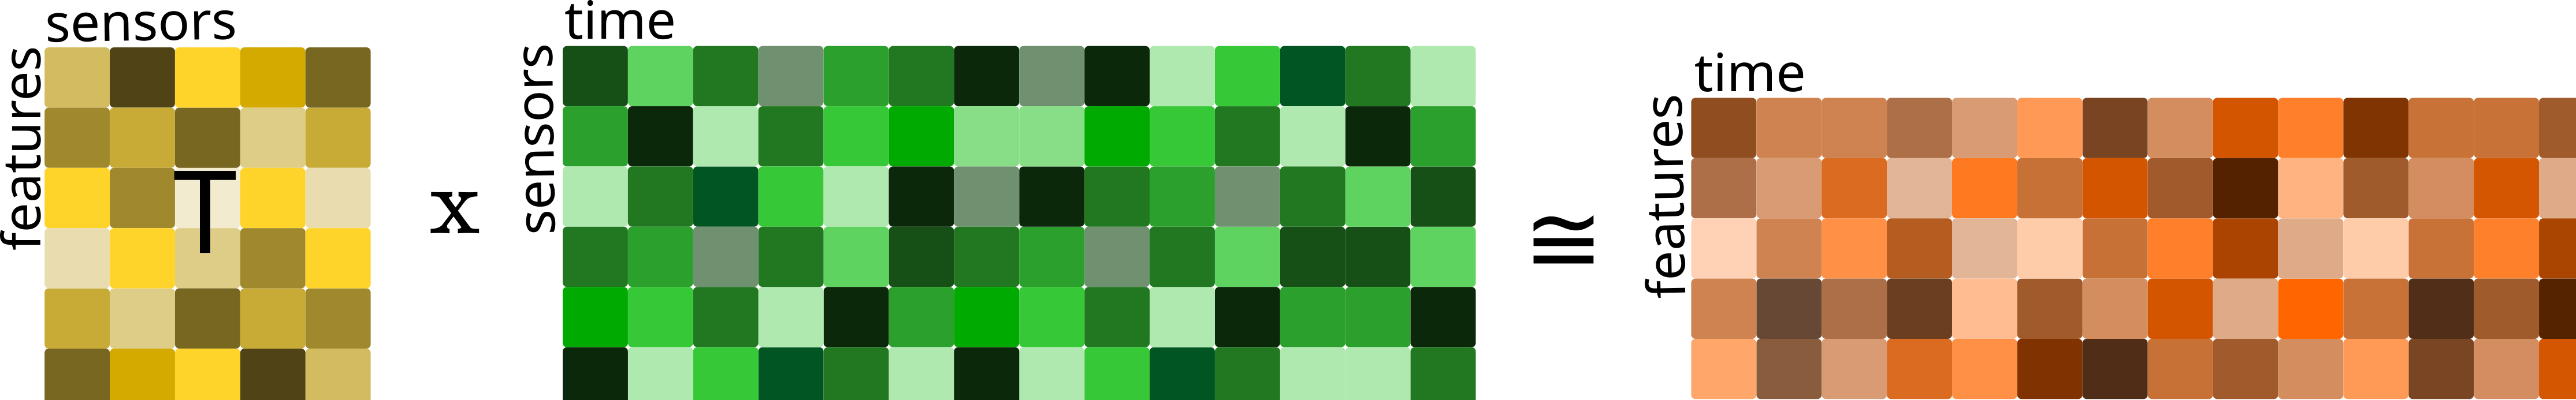
\includegraphics[width=\textwidth]{memento/spectral_srm/spectral_srm_basics_2.png}
		\caption{Transforming time resolved data into the shared space}
		\label{fig:spectral-srm2}
	\end{subfigure}
	\caption[Spectral shared response modeling]{Spectral shared response modeling: A shared response model decomposes spectral neural data (\ref{fig:spectral-srm1}, green) into a shared spectral space (features by frequencies; orange) and subject-specific basis (sensors by features; yellow). Because the subject specific bases transform sensor data independent on whether it is time resolved or spectral, they can be used to transform time resolved data (\ref{fig:spectral-srm2}; green) into time courses of the shared response spaces features.}
	\label{fig:spectral-srm}
\end{figure}

\subsection{Simulation study}


\begin{figure}
	\begin{subfigure}{1.0\textwidth}
		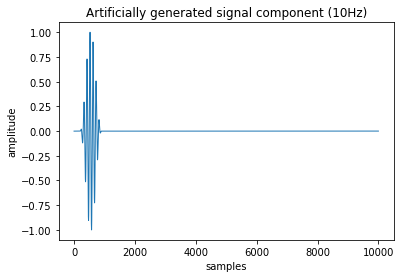
\includegraphics[width=.5\textwidth]{memento/simulation/sim_0.png}
		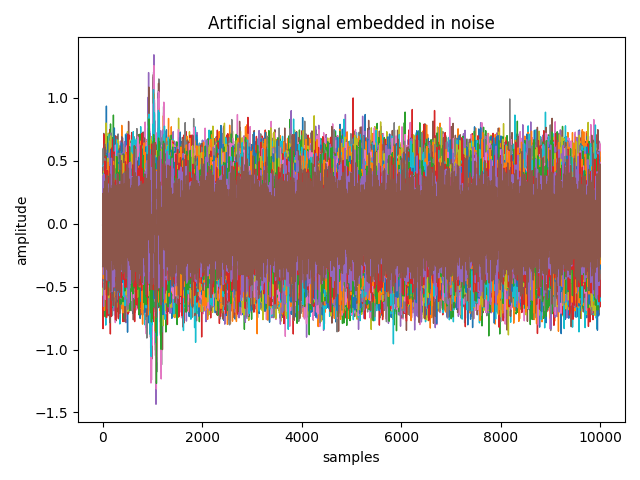
\includegraphics[width=.46\textwidth]{memento/simulation/sim_10.png}
	\end{subfigure}
	\caption{An artificial signal with 100000 samples and a 1000 sample spanning 10Hz main frequency component, pure (left) or partially embedded into 306 sensors with Gaussian noise (right). Roughly 20 percent of sensors contain the main signal in varying amounts, mirroring how brain signals are only present in certain sensors, and only in different strengths.}
	\label{fig:sim_artificial_signal}
\end{figure}

The following basic simulation illustrates the method:
In order to simulate \gls{meg} data from several subjects with a common frequency component that occurs at different points in time, we generate one ``ground truth'' signal with the same frequency and wave form, and embed it partially into 306 artificial sensors with Gaussian noise (Figure \ref{fig:sim_artificial_signal}).
To mirror how brain signals are only present in certain sensors and not with the same strength everywhere, only a fixed amount of sensors receives the signal.
For each sensor with a signal, a random weight between is drawn that determines the strength with which the signal is scaled.
This is repeated for N artificial subjects, but with a different random phase offset in the signal for each.
If the \gls{SRM} is successful, the shared response should reflect the ground truth signal despite phase offsets, and the subject-specific model bases should reflect the magnitudes of the weights for each sensor.\\
Using this data as the basis for shared response modeling, we now fit a probabilistic \gls{SRM} with $k=10$ features to recover the 10Hz signal as a shared component - either on time resolved data (Figure \ref{fig:sim-timeresolved}), or after transforming the data into its frequency spectrum (Figure \ref{fig:sim-spectral}).\\
When fit on time resolved data with phase shifts, the resulting shared space consists of components that differentially picked up signals from one or more participants, but represent it in a time series of repeated or overlapping signals.
This makes an interpretation of individual components difficult (Figure \ref{fig:sim-timeresolved-shared}).
The sensor weights that the model estimates for each component also do not show a clear association with the true weights used in the generation of the artificial data (Figure \ref{fig:sim-timeresolved-weights}).
In other words, with phase shifts between individual simulations' signals, different components of the shared space capture several participants' signals, but no \textit{general} ground truth signal.

\begin{figure}
	\begin{subfigure}{.49\textwidth}
		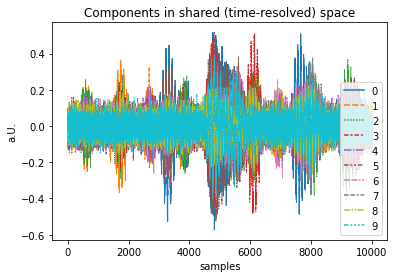
\includegraphics[width=\textwidth]{memento/simulation/sim_3.png}
		\caption{Shared space from time-resolved data}
		\label{fig:sim-timeresolved-shared}
	\end{subfigure}
	\begin{subfigure}{0.49\textwidth}
		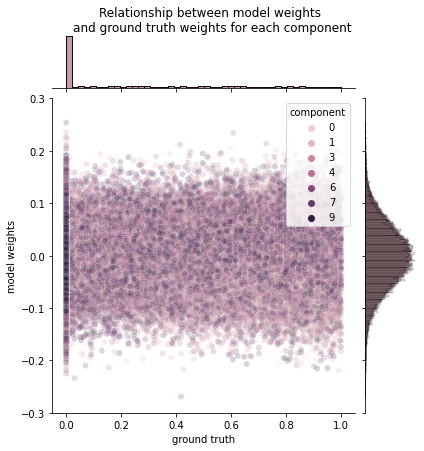
\includegraphics[width=\textwidth]{memento/simulation/sim_4.png}
		\caption{Recovered versus true weights}
		\label{fig:sim-timeresolved-weights}
	\end{subfigure}
	\caption{Outcome of fitting an \gls{SRM} on time resolved data with phase shifts: The components in shared space fail to capture a single ground truth, but show several subject's signals as consecutive or overlapping activity. The relationship between model weights and ground truth weights appears mostly random.}
	\label{fig:sim-timeresolved}
\end{figure}


However, transforming the signal into its frequency components, the spectral space, removes timing information, and with it, the phase offsets.
While the components in spectral space are not easy to interpret or differentiate (see Figure \ref{fig:sim-spectral-shared}), the scatterplot reveals that certain components' weights show a clear association to the weights used for model generation \ref{fig:sim-spectral-weights}.\\
This becomes apparent when shared components are visualized as time series by using the subject-specific weight matrices of the \gls{SRM} and individual subject's time-resolved data.
One or few components are consistently representing the original signal well across subjects, laying the basis for both identifying shared signal in phase-shifted data and interpreting the shared components resulting from it.


\begin{figure}
	\begin{subfigure}{.44\textwidth}
		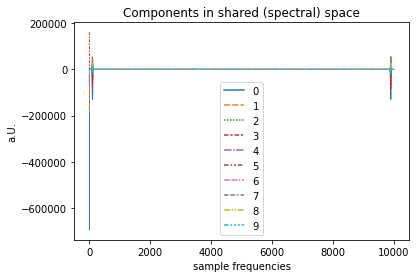
\includegraphics[width=\textwidth]{memento/simulation/sim_5.png}
			\caption{Shared space from spectral data}
		\label{fig:sim-spectral-shared}
	\end{subfigure}
	\begin{subfigure}{0.49\textwidth}
		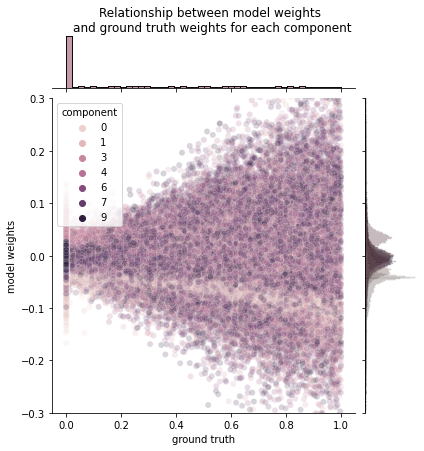
\includegraphics[width=\textwidth]{memento/simulation/sim_6.png}
			\caption{Recovered versus true weights}
		\label{fig:sim-spectral-weights}
	\end{subfigure}
	\hfill
	\begin{subfigure}{1.\textwidth}
		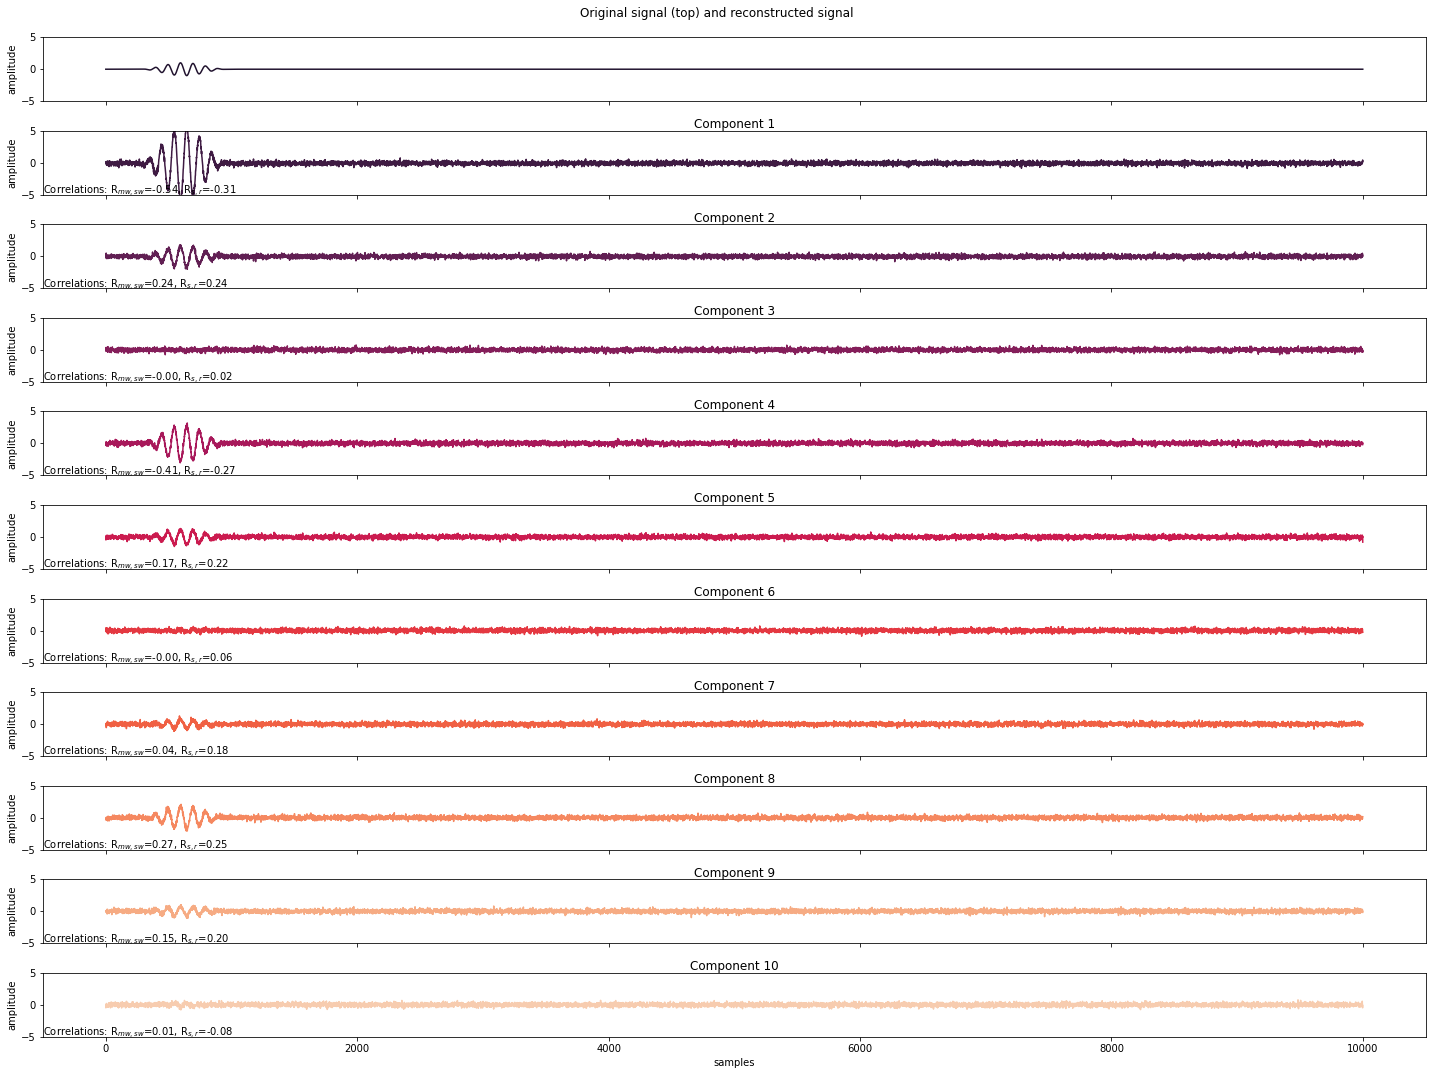
\includegraphics[width=.45\textwidth]{memento/simulation/sim_7.png}
		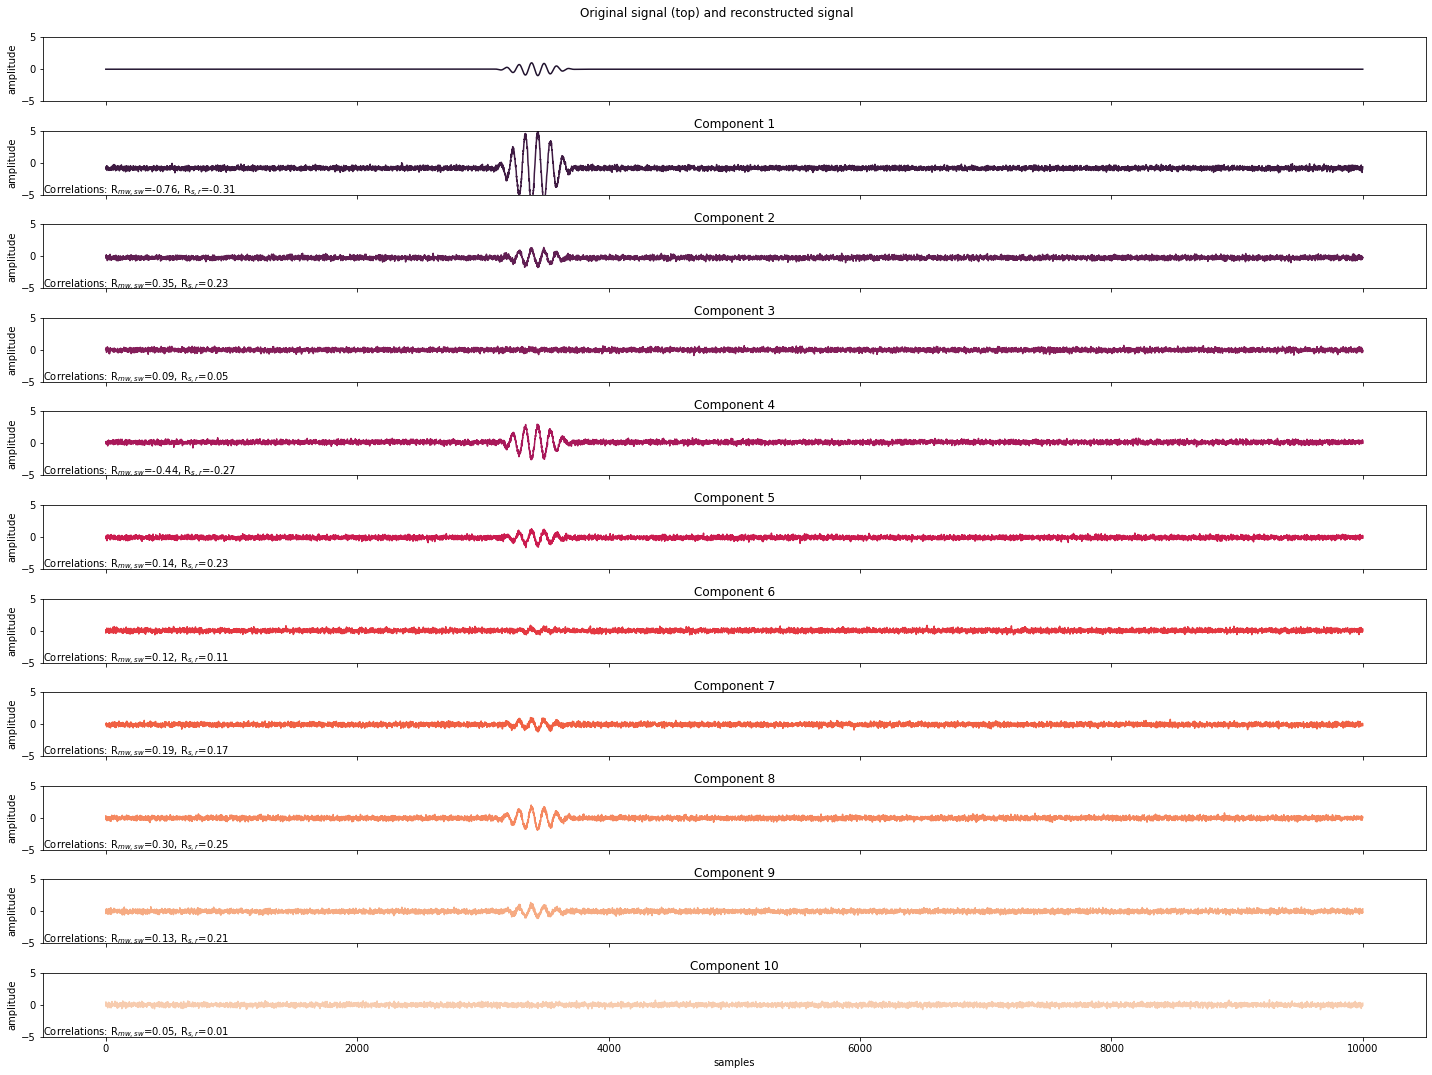
\includegraphics[width=.45\textwidth]{memento/simulation/sim_8.png}
		\caption{Shared components from \ref{fig:sim-spectral-shared}, visualized by transforming time resolved data of two different subjects}
		\label{fig:sim-spectral-transformed}
	\end{subfigure}
	\caption{Outcome of fitting an \gls{SRM} on spectrally transformed data: The components in shared space are spectral and difficult to interpret. But the relationship between model weights and ground truth weights clearly captures an association for some of the $k=10$ components. When time-resolved data from two different subjects is transformed using the subject specific bases from the \gls{SRM}, the individual subject's offset re-emerges.}
    \label{fig:sim-spectral}
\end{figure}


\subsection{Shared response modeling in spectral space on real data}

After the simulation study demonstrated principal feasibility of the method, I subsequently applied it to the neural recordings from the memento study.
The underlying aim was to investigate how decision-relevant properties are represented in working memory throughout the delay phase.
This was done with several exploratory analysis that followed the same general principle:
In a first step, data was split into a training and a test set.
For this, epochs were shuffled and randomly drawn to not introduce experiment fatigue as a confound.
A probabilistic shared response model was then fit on the spectrally transformed training data, yielding a shared spectral space (features by frequencies) and subject-specific basis (sensors by features) (\ref{fig:spectral-srm1}).
Importantly, the model had never seen the test data.
Using the subject-specific bases, the time-resolved test data was then transformed in the shared space while retaining the temporal resolution (\ref{fig:spectral-srm2}) to visualize the components the shared response model found.





\pagebreak

\section{Temporal decoding}

From Grootswagers et al. (2017): MVPA for MEG/EEG
The term “multivariate pattern analysis” (or MVPA) en-
compasses a diverse set of methods for analyzing neuro-
imaging data. The common element that unites these
approaches is that they take into account the relation-
ships between multiple variables (e.g., voxels in fMRI or
channels in MEG/EEG), instead of treating them as inde-
pendent and measuring relative activation strengths. The
term “decoding” refers to the prediction of a model from
the data (“encoding” approaches do the reverse, predict-
ing the data from the model, reviewed in Naselaris, Kay,
Nishimoto, \& Gallant, 2011; see also, e.g., Ding \& Simon,
2012, for an example of encoding models for MEG). The
most common application of decoding in cognitive neu-
roscience is the use of machine learning classifiers (e.g.,
correlation classifiers (Haxby et al., 2001) or discriminant
classifiers (Carlson et al., 2003; Cox \& Savoy, 2003) to
identify patterns in neuroimaging data, which correspond
to the experimental task or stimulus. The most popular
applications of MVPA are decoding (for recent reviews on
fMRI decoding, see e.g., Haynes, 2015; Pereira et al., 2009)
and, more recently, representational similarity analysis
(RSA: Kriegeskorte \& Kievit, 2013).

\subsection{machine learning concepts in scikit-learn}

\texttt{y} is the \textit{target}, also called \texttt{outputs}, \texttt{responses}, \texttt{label} or \texttt{ground truth}.¸ Its the \texttt{dependent variable} in supervised learning, passed to an \texttt{estimator}'s fit method as y.
\texttt{X} is the observed data. Its number of rows are the number of \texttt{samples}.
\texttt{features} are the individual elements of a vector representing a sample. In a data matrix, features are represented as columns. Elsewhere features are also known as attributes, predictors, regressors, or independent variables.
\texttt{samples} typically denote a single feature vector. Elsewhere, a sample is called an instance, data point, or observation. \texttt{n\_samples} indicates the number of samples in a dataset, being the number of rows in a data array \texttt{X}


A \texttt{classifier} is a predictor with a finite set of discrete possible output values, and must implement "fit", "predict", and "score" methods, and could implement "decision\_function", "predict\_proba" and "predict\_log\_proba" methods.
An \texttt{estimator} is an object that manages the estimation and decoding of a model. An estimators fit method takes samples X, target y, and sample properties (e.g., weights). Once fitted, the "predict\_proba" method can return probability estimates for each class from some input data X. A \texttt{score} is a method that evaluates predictions on a given dataset, returning a single

\texttt{evaluation metrics} accept a ground truth and a prediction (e.g., output of predict, predict\_proba, etc)

\texttt{Transformers} (or \texttt{transforms}) can clean, reduce, expand, or generate feature representation.
 is
\texttt{Pipelines} sequentially chain transforms with a final estimator, and reduce the possibilities of forgetting transformations that could lead to inconsistent preprocessing applications between training and testing data and of leaking test data into training data. The purpose of a pipeline is to assemble several steps that can be cross-validated together whiule

\section{Results}
\pagebreak

\section{Discussion}
For the past decades, scientific publishing has favored significant over nonsignificant findings \citep{dwan2008systematic}, a condition termed \textit{publication bias} or \textit{file drawer problem} \citep{rosenthal1979file}.

Low statistical power reduces not only the likelihood to find a true effect, but also the likelihood that statistically significant results reflect a true effect \citep{button2013power}.
And as increased noise in small samples inflates the effect size of significant results \citep{loken2017measurement}, published low-powered studies likely overestimate the
% !TeX root = ../main-english.tex
% !TeX spellcheck = en-US
% !TeX encoding = utf8
% -*- coding:utf-8 mod:LaTeX -*-

%This smart spell only works if no changes have been made to the chapter
%using the options proposed in preambel/chapterheads.tex.
\setchapterpreamble[u]{%
	\dictum[Isaac Newton]{If I have seen further it is by standing on the shoulders of Giants}
}

\chapter{Conclusion}
\label{discussion}

The original aim of this work was to find novel insights about brain state transitions in a delayed decision making task from previously unpublished data by connecting and building up on prior work by other researchers.
However, the context in which this project was conducted made research data management and research software engineering more central than originally planned.
Viewed in conjunction, this thesis has been a testament to the foundational importance that organizational and technical aspects of scientific conduct play in research endeavors.\\
Chapter \ref{chap:k1} laid out an overview of the study of working memory maintenance, in particular novel methods that viewed neural signals as trajectories through high-dimensional state spaces.
It further introduced preexisting tools and solutions for managing research data and projects.
The \gls{FAIR} principles and the \gls{BIDS} standard are established elements of good \gls{rdm}, and DataLad a promising software tool for data versioning, transport, and digital provenance capture.
In conjunction, they enable researchers to create scientific outputs that are portable and reusable as stand-alone, well-described units, without reliance on the original authors -- and thus, a fitting tool set to conduct the brain-state analysis in Chapter \ref{chap:k4}.\\
However, Chapter \ref{chap:k1} also shed light on DataLad's shortcomings and deficiencies.
Thus, my work on the DataLad Handbook, outlined in Chapter \ref{chap:k2} and rooted in the area of research software engineering, improved some of these with documentation and workflows.
This constituted not only a beneficial foundation for my own DataLad-supported analysis in Chapter \ref{chap:k4}, but also led to lasting resources for the general public and improved software usabibility.
The Handbook's popularity and its association with increased relevance of the software tool yielded evidence for the importance of user-focused documentation.
Although this work is not a traditional academic paper, it can, similar to research software, published findings, or open code impact scientific conduct positively.\\
Continuing in a similar spirit, Chapter \ref{chap:k3} focused on two central aspects in research data management, specifically reusability and reproducibility, and showed how they connected to each other:
Reproducibility is a basis for reusability, and both are the outcome of research data management that becomes increasingly more FAIR.
But Chapter \ref{chap:k3} also outlined the practical difficulties of creating reusable research outputs that arise despite the existence of the \gls{FAIR} principles because full FAIRness can not always be achieved.
To address them, I conceived a set of four pragmatic research data management strategies that can make research objects more reusable, even when they are not yet fully \gls{FAIR}.
While our work recognizes the FAIR principles, it makes a pragmatic compromise between the aspirational ideal state, and the continuously developing research and meta data landscape in computational sciences.
In passing, as a byproduct of \gls{rdm}, its outcomes go a long way towards FAIR, and by applying the four properties of exhaustively versioned, actionable, modular and portable to research projects, become re-usable by default.
Chapter \ref{chap:k3} then concluded with a computational framework that put these strategies into practice, and highlighted our proof of principle work to test its applicability and scalability on a neuroscientific dataset of the largest scale.\\
Our framework brought together a range of work that the previous chapters outlined already.
At the center of our framework lies thoughtful research data and reproducibility management, not as an afterthought, but -- given the technical challenges computational reproducibility poses -- as a sturdy and necessary basis.
In the spirit of reusable and FAIR digital research objects, it creates outcomes that lend themselves to reuse naturally.
Especially in large-scale computations, current results will be the inputs of future projects, and their built-in reusability provides the necessary trust for this.
The introduction also established DataLad as a software tool to deliver this research data management.
Its development principles and features in the spirit of decentralized software development translate into utility for our framework.
For one, it is able to connect a range of established services or and open source tools to ease adoption and maximize flexibility.
And although the workflows and concepts our framework draws from are not based in the domain of reproducible data processing, they lend themselves well for this application, and what made distributed software development productive, fast, and reliable, now helps to do the same for data analysis.
Fundamental to the success and usability of DataLad and its use in this framework is its documentation, as argued in Chapter \ref{chap:k2}.
On a high level, the framework constitutes yet another use case, only possible because the tools' features are combined into something greater than the sum of its parts.
Many years of refining user-centered workflows and software usability formed the basis for this.
The available documentation allows interested readers to learn beyond the publication, up to a point where they can extend it to their own use cases.
A testament to this, and to the utility of the framework is its adoption into dedicated new tools already in an early stage of its development.
\citet{heunis2023catalog} makes use of it for reproducible metadata aggregation, it plays a role in the CuBIDS packages for the reproducible curation of \gls{BIDS} datasets \citep{covitz2022curation}, and a dedicated software tool, BABS, has been created to improve the usability of the workflow even more \citep{zhao2023reproducible}.\\
Chapter \ref{chap:k4} then put the technical and organizational work of previous chapters into action.
The idiosyncratic structure of the \textit{memento} dataset has posed a significant challenge to identify relevant files, distinguish processing states, understand the dataset as a whole, and base processing on it.
The conversion to the \gls{BIDS} standard for \gls{meg} was an indispensable prerequisite to working with this data.
The spatio-temporally distributed nature of the project, spread over three institutions and two generations of researchers working with the dataset, placed reusability and portability demands on my work that the previous chapters laid the foundations to.
I was unable to find the delay representation of stimulus properties which the experiment had originally set out to find.
However, I was able to extend previous analyses with novel ideas, methods that are yet unconventional in \gls{meg}, and interesting exploratory findings that can spark further research.
With the \gls{rdm} principles I theorized in Chapter \ref{chap:k3}, documented in Chapter \ref{chap:k2}, helped to software engineer in Chapter \ref{chap:k1}, and applied in Chapter \ref{chap:k4}, future re-users can obtain or recompute my results, or investigate differences between re-computations after adjusting pipelines or parametrization with novel research ideas.
The intermediate research outcomes of this project thus are a valuable stepping stone for further research.





%For the past decades, scientific publishing has favored significant over nonsignificant findings \citep{dwan2008systematic}, a condition termed \textit{publication bias} or \textit{file drawer problem} \citep{rosenthal1979file}.






%Low statistical power reduces not only the likelihood to find a true effect, but also the likelihood that statistically significant results reflect a true effect \citep{button2013power}.
%And as increased noise in small samples inflates the effect size of significant results \citep{loken2017measurement}, published low-powered studies likely overestimate the effects that they report.
%In a systematic review by \citet{pavlov2022oscillatory}, the average number of participants in experimental studies of verbal or visual working memory was $N_{verbal}=19.3$ and $N_{visual}=23.3$, respectively.

%However, \citet{pavlov2022oscillatory} highlighted the lack of agreement in the field in a systematic review recently, and pointed to various confounding factors in past studies. They outlined, for example, that gamma band oscillations found in \gls{eeg} studies are more likely to be muscle components.
%This uncertainty makes it difficult to hypothesize.







\printbibliography


\appendix
% !TeX encoding=utf8
% !TeX spellcheck = en-US

\chapter{Publications}
%\markboth{Publications}{Publications}

The following publications and conference contributions of mine were relevant for the thesis at hand.

%% In these lists the publications are numbered by date of publications
%% and the author of the thesis can be printed in bold.

\section*{Scientific publications}
% \section*{Wissenschaftliche Veröffentlichungen}
\begin{refsection}
\nocite{Halchenko2021, NISO2022119623, HankePestilliWagnerMarkiewiczPolineHalchenko+2021+17+25, wagner2020datalad, wagner2022fairly}
\begin{refcontext}[sorting=nyt]  
	\printbibliography[heading=none, resetnumbers=true]
\end{refcontext}
\end{refsection}

\section*{Submissions to international conferences}
% \section*{Beiträge auf internationalen Konferenzen}
\begin{refsection}
\nocite{wagner202310, wagnerohbm2022, wagnerohbm2021, poldrackohbm2020, wagner_adina_s_2020_7906718}

%\printbibliography[env=numbered+bold, heading=none, sorting=ynt, resetnumbers=true]
\begin{refcontext}[sorting=nyt]  
	\printbibliography[heading=none, resetnumbers=true]
\end{refcontext}
\end{refsection}

\section*{Submissions to national conferences}
% \section*{Beiträge auf nationalen Konferenzen}
\begin{refsection}
\nocite{adina_s_wagner_2021_4541323}

%\printbibliography[env=numbered+bold, heading=none, sorting=ynt, resetnumbers=true]
\begin{refcontext}[sorting=nyt]  
	\printbibliography[heading=none, resetnumbers=true]
\end{refcontext}


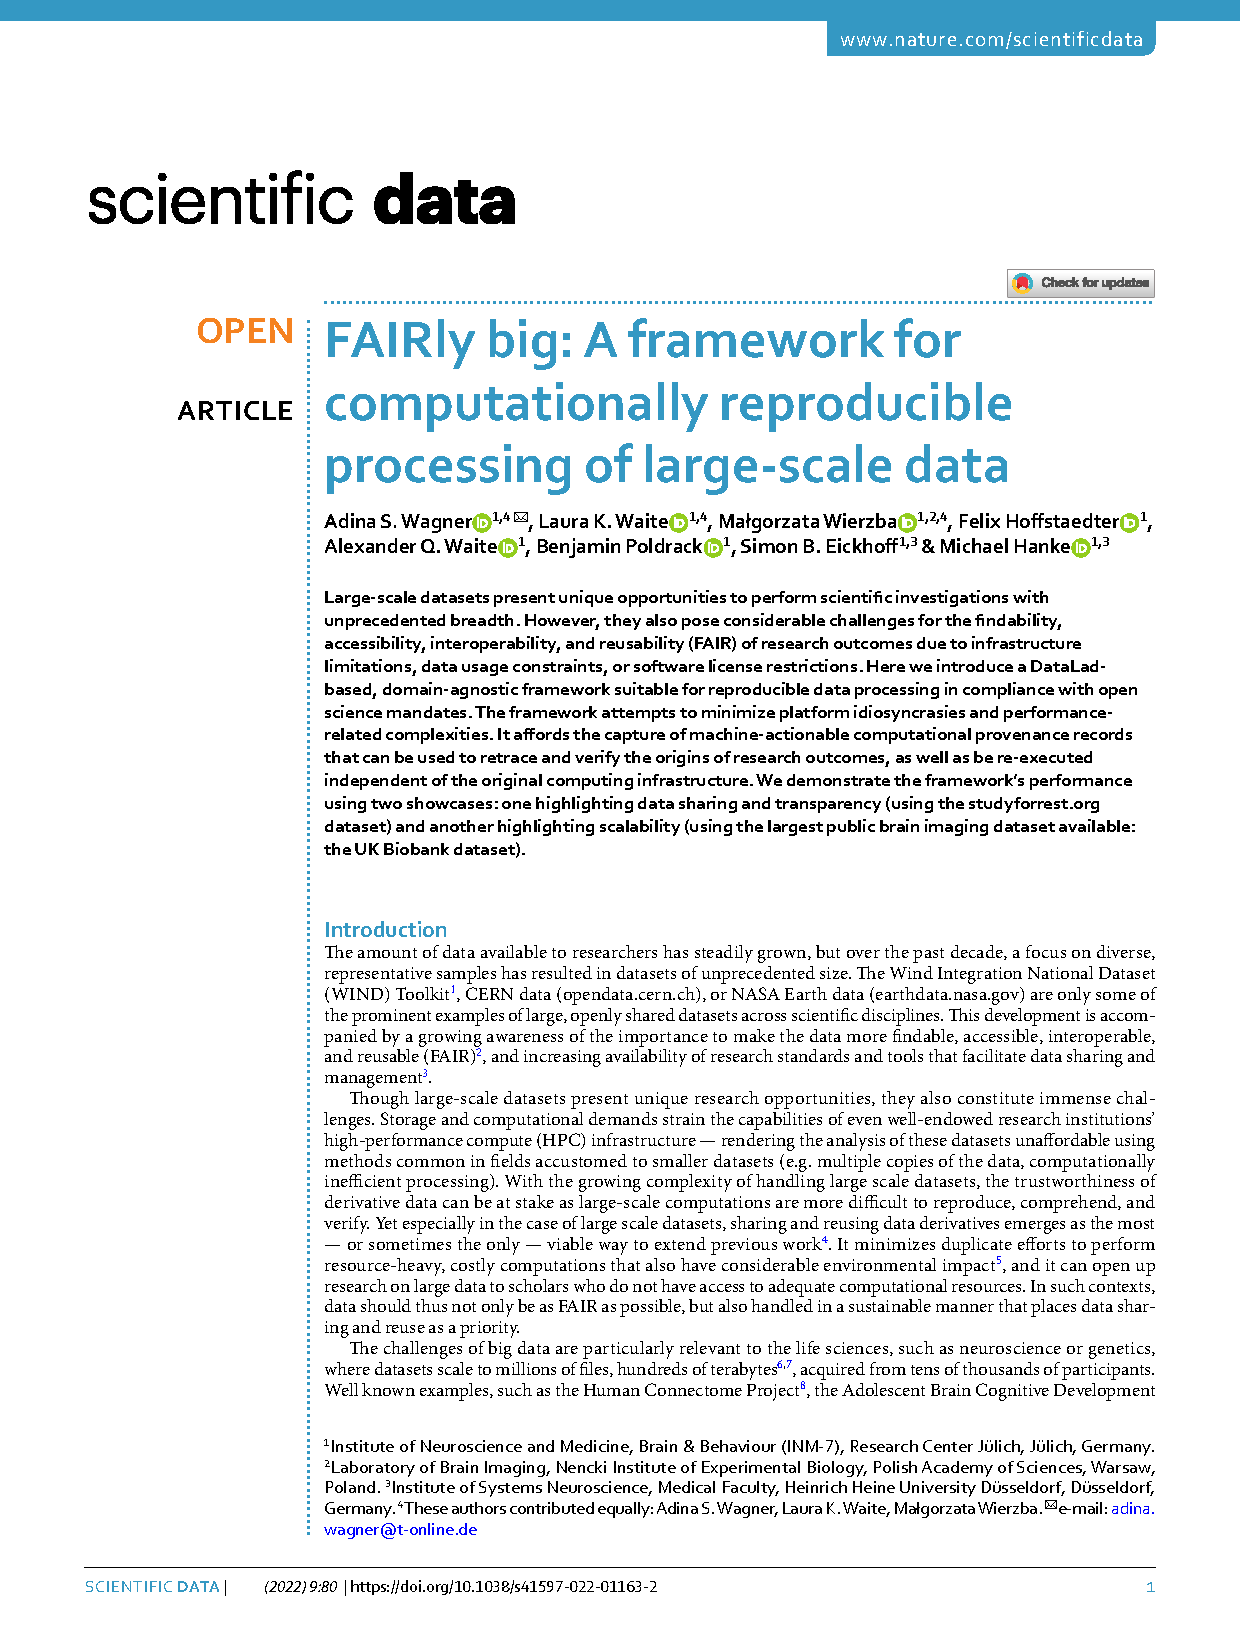
\includepdf[pages=1-17]{content/appendix_pub_fairlybig.pdf}
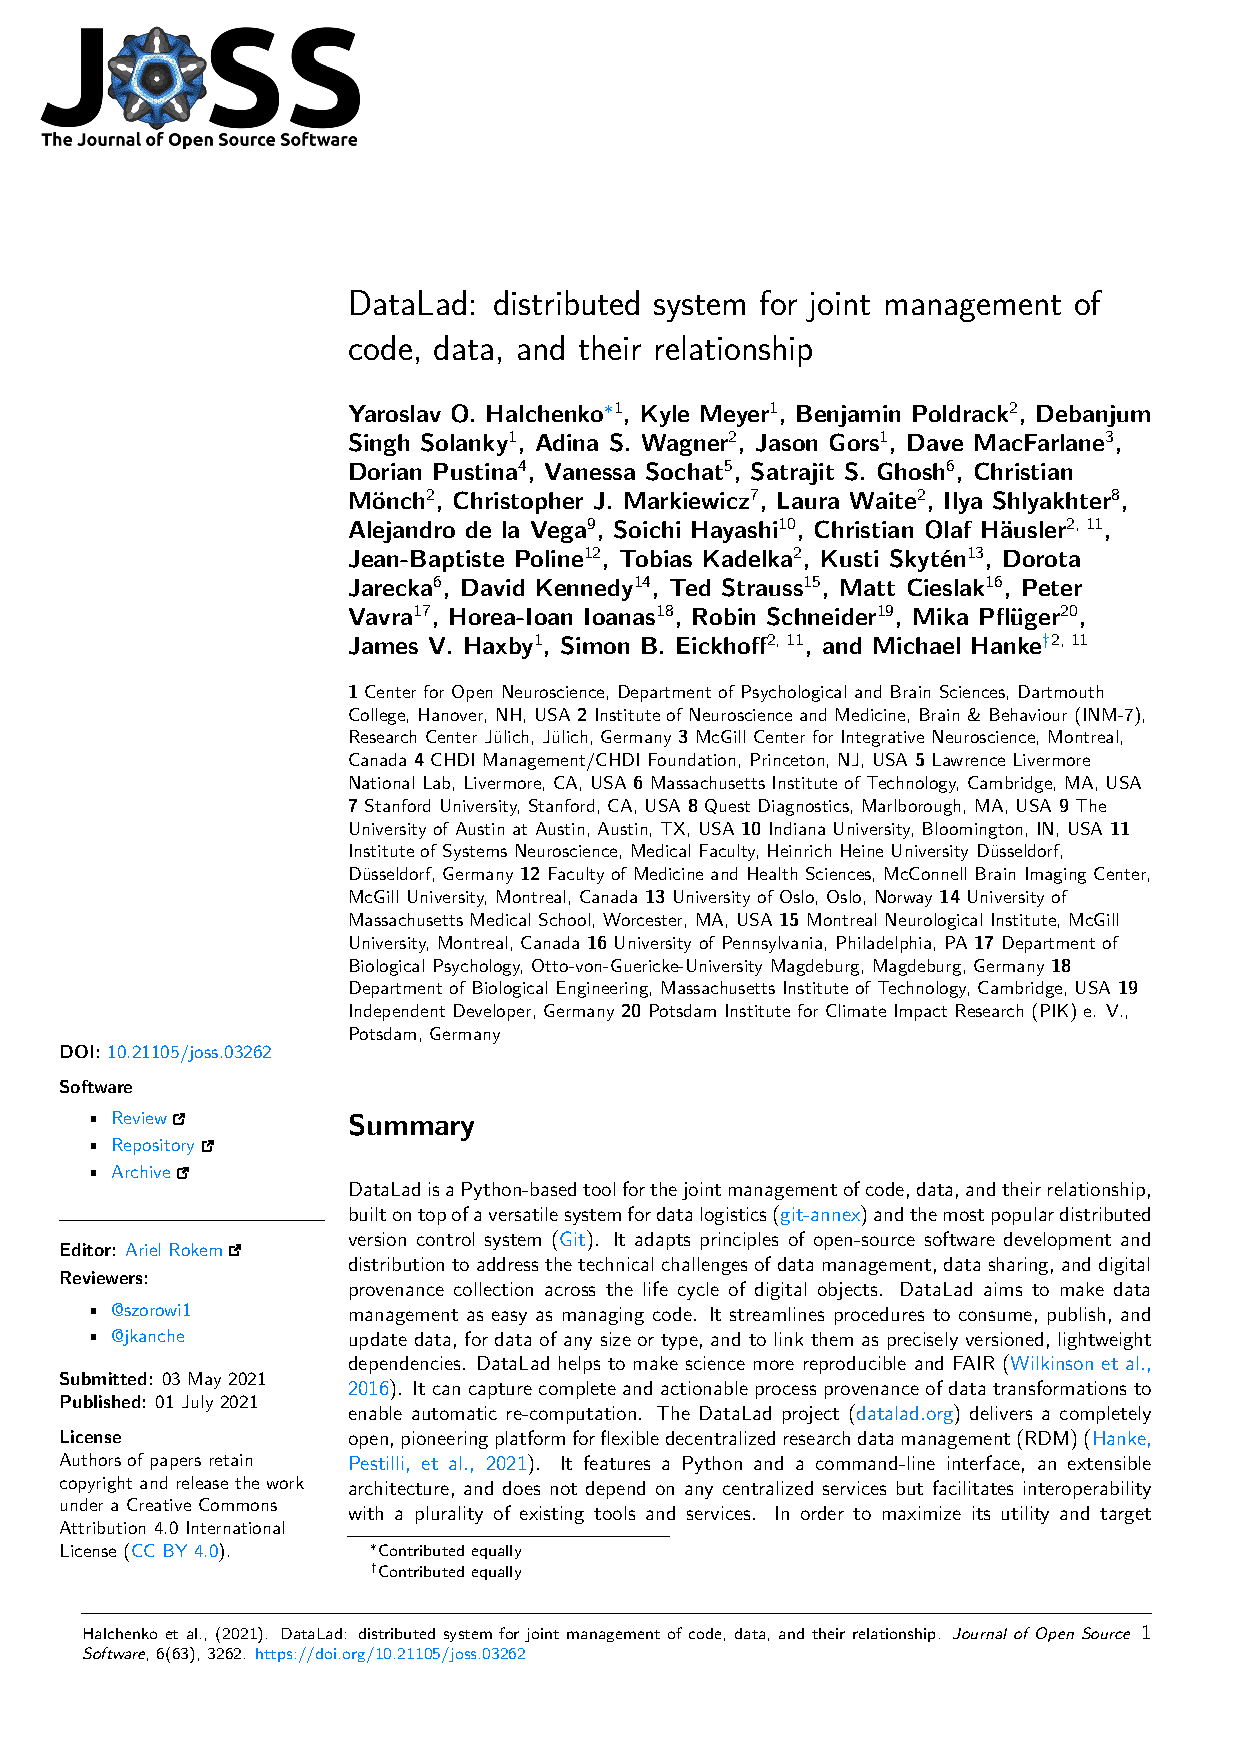
\includepdf[pages=1-8]{content/appendix_pub_datalad.pdf}

\end{refsection}
%

% !TeX root = main-english.tex
% !TeX spellcheck = en-US
% !TeX encoding = utf8
% -*- coding:utf-8 mod:LaTeX -*-

%This smart spell only works if no changes have been made to the chapter
%using the options proposed in preambel/chapterheads.tex.
\setchapterpreamble[u]{%
  \dictum[Albert Einstein]{We cannot solve our problems with the same level of thinking that created them}
}
\chapter{LaTeX Hints}
\label{chap:latexhints}

One sentence per line.
This rule is important for the usage of version control systems.
A new line is generated with a blank line.
As you would do in Word:
New paragraphs are generated by pressing enter.
In LaTeX, this does not lead to a new paragraph as LaTeX joins subsequent lines.
In case you want a new paragraph, just press enter twice (!).
This leads to an empty line.
In word, there is the functionality to press shift and enter.
This leads to a hard line break.
The text starts at the beginning of a new line.
In LaTeX, you can do that by using two backslashes (\textbackslash\textbackslash).
This is rarely used.

Please do \textit{not} use two backslahes for new paragraphs.
For instance, this sentence belongs to the same paragraph, whereas the last one started a new one.
A long motivation for that is provided at \url{http://loopspace.mathforge.org/HowDidIDoThat/TeX/VCS/#section.3}.

One can write \emph{emphasized text (rendered in italics)} and \textbf{bold text}.

\section{File Encoding and Support of Umlauts}
\label{sec:firstsectioninlatexhints}
The template offers foll UTF-8 support.
All recent editors should not have issues with that.

\section{Citations}


References are set by means of \texttt{\textbackslash cite[key]}.

\begin{filecontents*}[overwrite]{\democodefile}
Example: \cite{WSPA} or by author input: \citet{WSPA}.
\end{filecontents*}
\PrintDemo{style=parallel}

The following sentence demonstrates
\begin{inparaenum}[1.]
  \item the capitalization of author names at the beginning of the sentence,
  \item the correct citation using author names and the reference,
  \item that the author names are a hyperlink to the bibliography and that
  \item the bibliography contains the name prefix \qq{van der} of \qq{Wil M.\,P.\ van der Aalst}.
\end{inparaenum}

\begin{filecontents*}[overwrite]{\democodefile}
\Citet{RVvdA2016} present a study on the effectiveness of workflow management systems.
\end{filecontents*}
\PrintDemo{style=parallel}

The following sentence demonstrates that you can overwrite the text part of the generated label using \texttt{label} in a bibliopgrahie"=entry, but the year and the uniqueness is still generated by biber.

\begin{filecontents*}[overwrite]{\democodefile}
The workflow engine Apache ODE \cite{ApacheODE} executes \BPEL processes reliably.
\end{filecontents*}
\PrintDemo{style=parallel}

\begin{filecontents*}[overwrite]{\democodefile}
Words are best enclosed using \texttt{\textbackslash qq\{..\}}, then the correct quotes are used.
\end{filecontents*}
\PrintDemo{style=parallel}

When creating the Bibtex file it is recommended to make sure that the DOI is listed.

\section{Formulas and Equations}
\label{sec:mf}

\begin{filecontents*}[overwrite]{\democodefile}
Equations $f(x)=x$ inside the text can be provided.
\end{filecontents*}
\PrintDemo{style=parallel}

A list with all available mathematical symbols is provided at \url{http://texdoc.net/pkg/symbols-a4}.

\begin{filecontents*}[overwrite]{\democodefile}
As example the set of natural numbers is given by $\mathbb{N}$.
\end{filecontents*}
\PrintDemo{style=parallel}

For the documentation of editing mathematical formulas read the package documentation of \texttt{amsmath}\footnote{\url{http://texdoc.net/pkg/amsmath}}.

Equation~\ref{eq:test} is numbered and can be referenced in the text:
\begin{filecontents*}[overwrite]{\democodefile}
\begin{align}
  \label{eq:test}
  x = y
\end{align}
\end{filecontents*}
\PrintDemo{style=parallel}

Following equation is not numbered because of using \texttt{\textbackslash align*} as environment.
\begin{filecontents*}[overwrite]{\democodefile}
\begin{align*}
  x = y
\end{align*}
\end{filecontents*}
\PrintDemo{style=parallel}

The template offers \verb+\abs+ to enable the bars scaling well at the absolute value:

\begin{filecontents*}[overwrite]{\democodefile}
$\abs{X}$.
\end{filecontents*}
\PrintDemo{style=parallel}

More details about mathematical environments provides the documentation available at \url{http://www.ctan.org/tex-archive/help/Catalogue/entries/voss-mathmode.html}.


%%%%%%%%%%%%%%%%%%%%%%%%%%%%%%%%%%%%%%%%%%%%%%%%%%%%%%%%%%%%%%%%%%%%%%%%%%%%%%
\section{Sourcecode}
%%%%%%%%%%%%%%%%%%%%%%%%%%%%%%%%%%%%%%%%%%%%%%%%%%%%%%%%%%%%%%%%%%%%%%%%%%%%%%
\Cref{lst:ListingANDlstlisting} shows how to emmbed source code.
With \texttt{\textbackslash lstinputlisting} the source code can be loaded directly from files.

%Listing-Umgebung wurde durch \newfloat{Listing} definiert
\begin{Listing}
  \begin{lstlisting}
<listing name="second sample">
  <content>not interesting</content>
</listing>
\end{lstlisting}
  \caption{The code is separated by two horizontal lines in the listings environment.}
  \label{lst:ListingANDlstlisting}
\end{Listing}

\begin{filecontents*}[overwrite]{\democodefile}
Source code is also available in the text \lstinline|<listing />|.
\end{filecontents*}
\PrintDemo{style=parallel}


%%%%%%%%%%%%%%%%%%%%%%%%%%%%%%%%%%%%%%%%%%%%%%%%%%%%%%%%%%%%%%%%%%%%%%%%%%%%%%
\section{Pseudocode}
%%%%%%%%%%%%%%%%%%%%%%%%%%%%%%%%%%%%%%%%%%%%%%%%%%%%%%%%%%%%%%%%%%%%%%%%%%%%%%
\Cref{alg:sample} shows a sample algorithm.
\begin{Algorithmus} %Use the environment only if you want to place the algorithm similar to graphics from TeX
  \caption{Sample algorithm}
  \label{alg:sample}
  \begin{algorithmic}
\Procedure{Sample}{$a$,$v_e$}
\State $\mathsf{parentHandled} \gets (a = \mathsf{process}) \lor \mathsf{visited}(a'), (a',c,a) \in \mathsf{HR}$
\State \Comment $(a',c'a) \in \mathsf{HR}$ denotes that $a'$ is the parent of $a$
\If{$\mathsf{parentHandled}\,\land(\mathcal{L}_\mathit{in}(a)=\emptyset\,\lor\,\forall l \in \mathcal{L}_\mathit{in}(a): \mathsf{visited}(l))$}
\State $\mathsf{visited}(a) \gets \text{true}$
\State $\mathsf{writes}_\circ(a,v_e) \gets
\begin{cases}
\mathsf{joinLinks}(a,v_e) & \abs{\mathcal{L}_\mathit{in}(a)} > 0\\
\mathsf{writes}_\circ(p,v_e)
& \exists p: (p,c,a) \in \mathsf{HR}\\
(\emptyset, \emptyset, \emptyset, false) & \text{otherwise}
\end{cases}
$
\If{$a\in\mathcal{A}_\mathit{basic}$}
  \State \Call{HandleBasicActivity}{$a$,$v_e$}
\ElsIf{$a\in\mathcal{A}_\mathit{flow}$}
  \State \Call{HandleFlow}{$a$,$v_e$}
\ElsIf{$a = \mathsf{process}$} \Comment Directly handle the contained activity
  \State \Call{HandleActivity}{$a'$,$v_e$}, $(a,\bot,a') \in \mathsf{HR}$
  \State $\mathsf{writes}_\bullet(a) \gets \mathsf{writes}_\bullet(a')$
\EndIf
\ForAll{$l \in \mathcal{L}_\mathit{out}(a)$}
  \State \Call{HandleLink}{$l$,$v_e$}
\EndFor
\EndIf
\EndProcedure
  \end{algorithmic}
\end{Algorithmus}

\clearpage
And if you want to write an algorithm that goes over several pages, you can only do this with the following \textbf{dirty} hack:

{
\begin{minipage}{\textwidth}
  \hrule height .8pt width\textwidth
  \vskip.3em%\vskip\abovecaptionskip\relax
  \stepcounter{Algorithmus}
  \addcontentsline{alg}{Algorithmus}{\protect\numberline{\theAlgorithmus}{\ignorespaces Description \relax}}
  \noindent\textbf{Algorithmus \theAlgorithmus} Description
  %\stepcounter{algorithm}
  %\addcontentsline{alg}{Algorithmus}{\thealgorithm{}\hskip0em Description}
  %\textbf{Algorithmus \thealgorithm} Description
  \vskip.3em%\vskip\belowcaptionskip\relax
  \hrule height .5pt width\textwidth
\end{minipage}
%without the following line, the text is nerer at the rule
\vskip-.3em
%
code goes here\\
test2\\
%
\vskip-.7em
\hrule height .5pt width\textwidth
}


%%%%%%%%%%%%%%%%%%%%%%%%%%%%%%%%%%%%%%%%%%%%%%%%%%%%%%%%%%%%%%%%%%%%%%%%%%%%%%
\section{Figures}
%%%%%%%%%%%%%%%%%%%%%%%%%%%%%%%%%%%%%%%%%%%%%%%%%%%%%%%%%%%%%%%%%%%%%%%%%%%%%%
The \cref{fig:chor1} and \ref{fig:chor2} are important to understand this document.
In the appendix \vref{fig:AnhangsChor} shows again the complete choreography.

%The parameters in square brackets are optional - e.g. [htb!]
%htb! means: Dear LaTeX, please place this image here first ("_h_ere"). If this does not work, place it at the "_t_op" of the page. And if this is not possible, please place it at the "_b_ottom" of the page. And please, please prefer here and above, even if it doesn't look so optimal ("!")
%These should NOT be used if possible. LaTeX's algorithm for placing the glide environment is already very good!
\begin{figure}
  \centering
  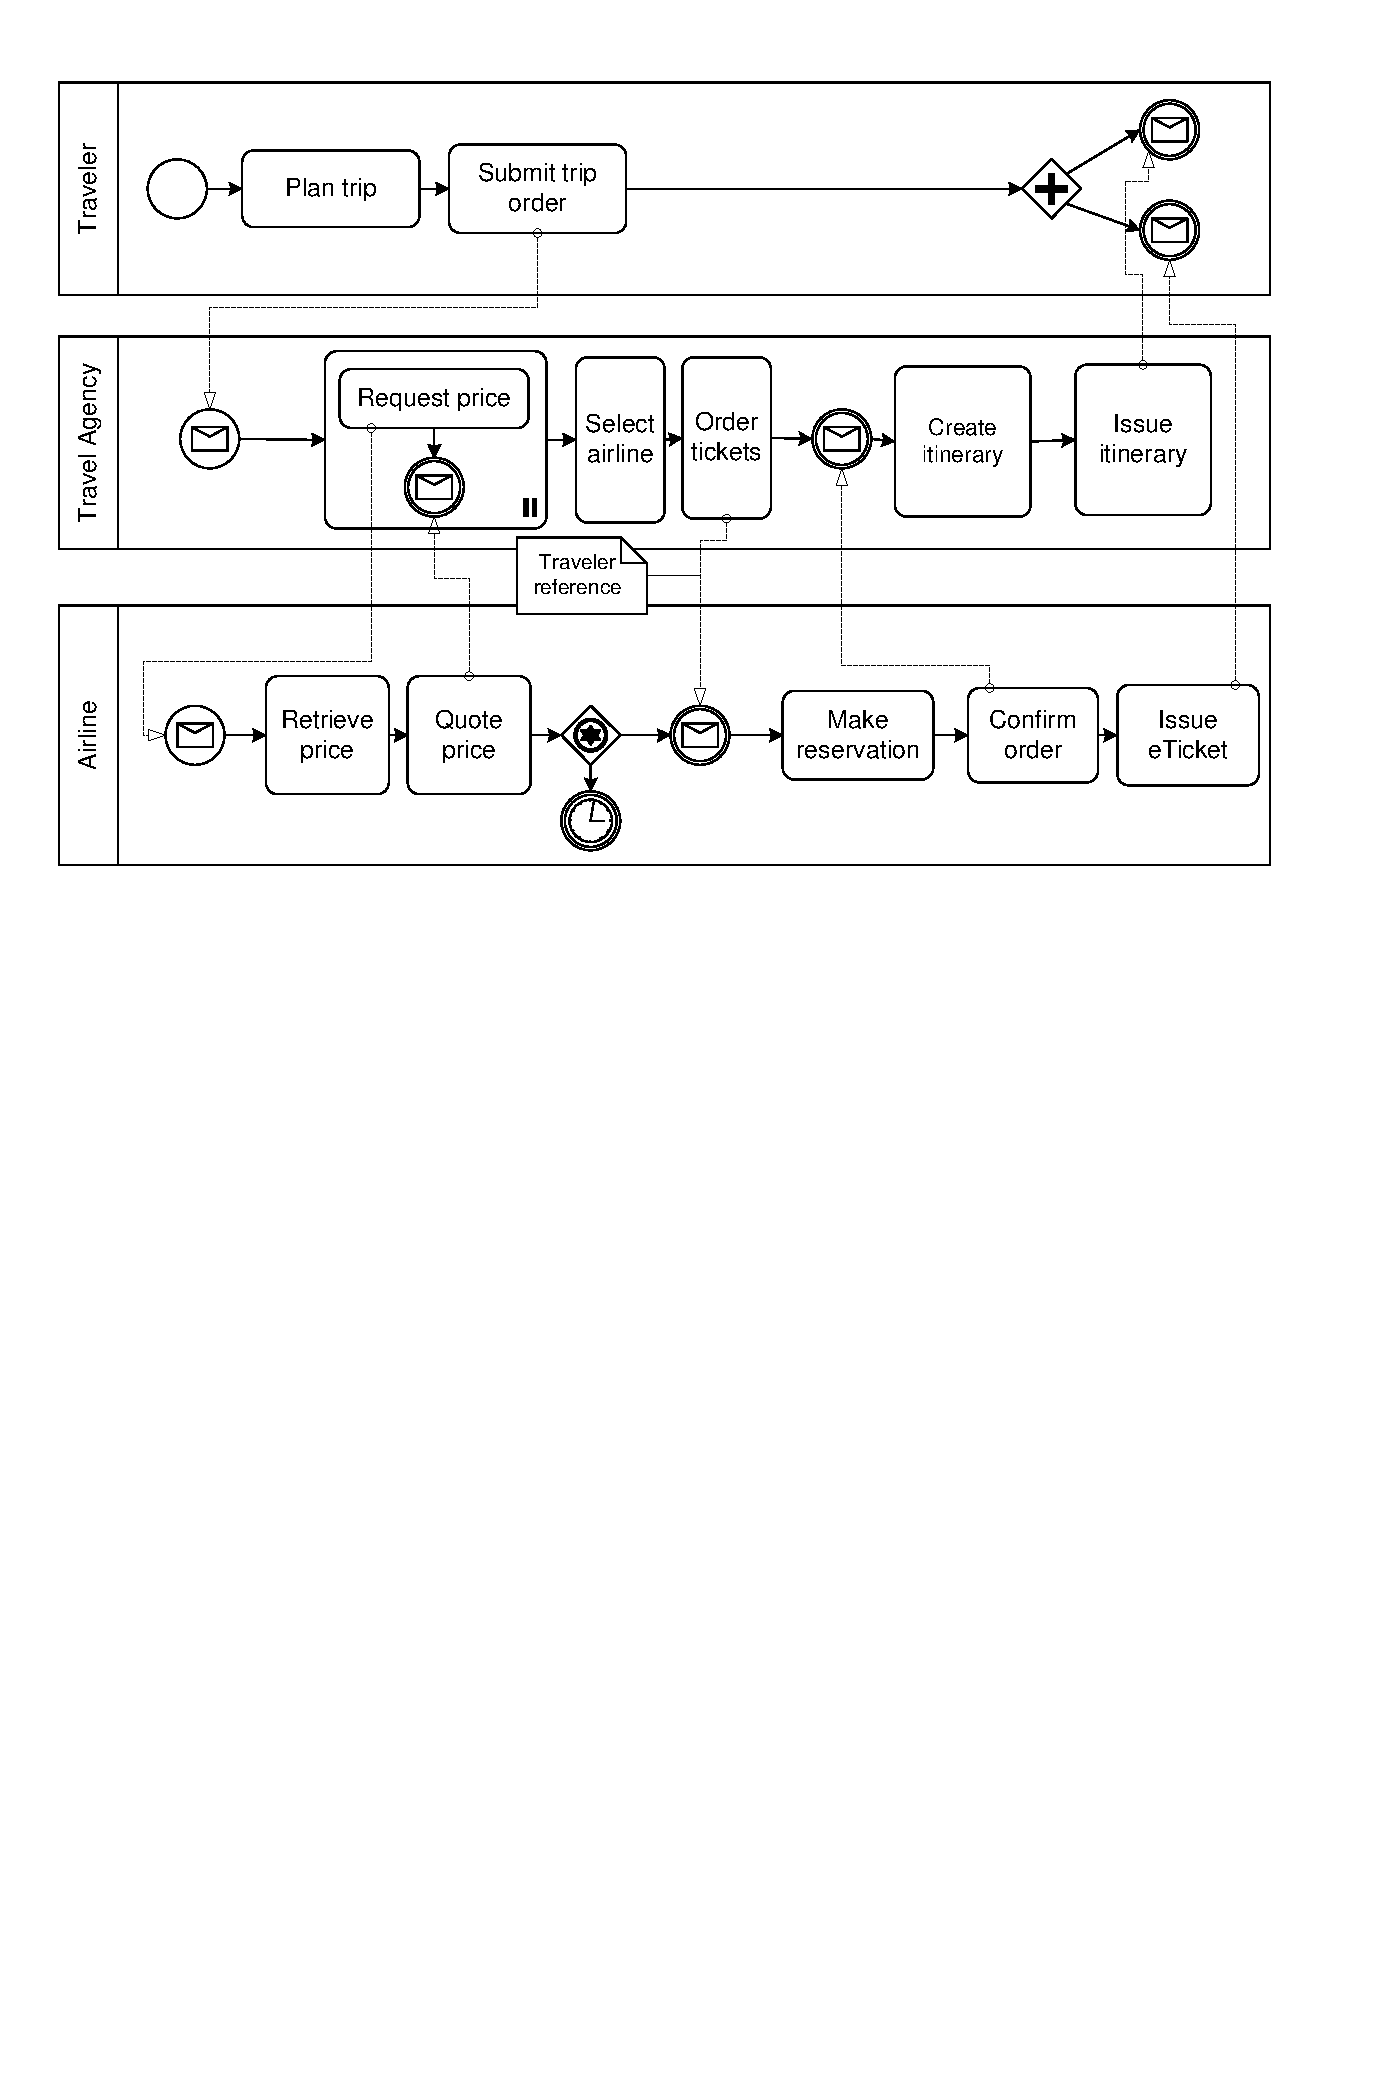
\includegraphics[width=\textwidth]{choreography.pdf}
  \caption{Example Choreography}
  \label{fig:chor1}
\end{figure}

\begin{figure}
  \centering
  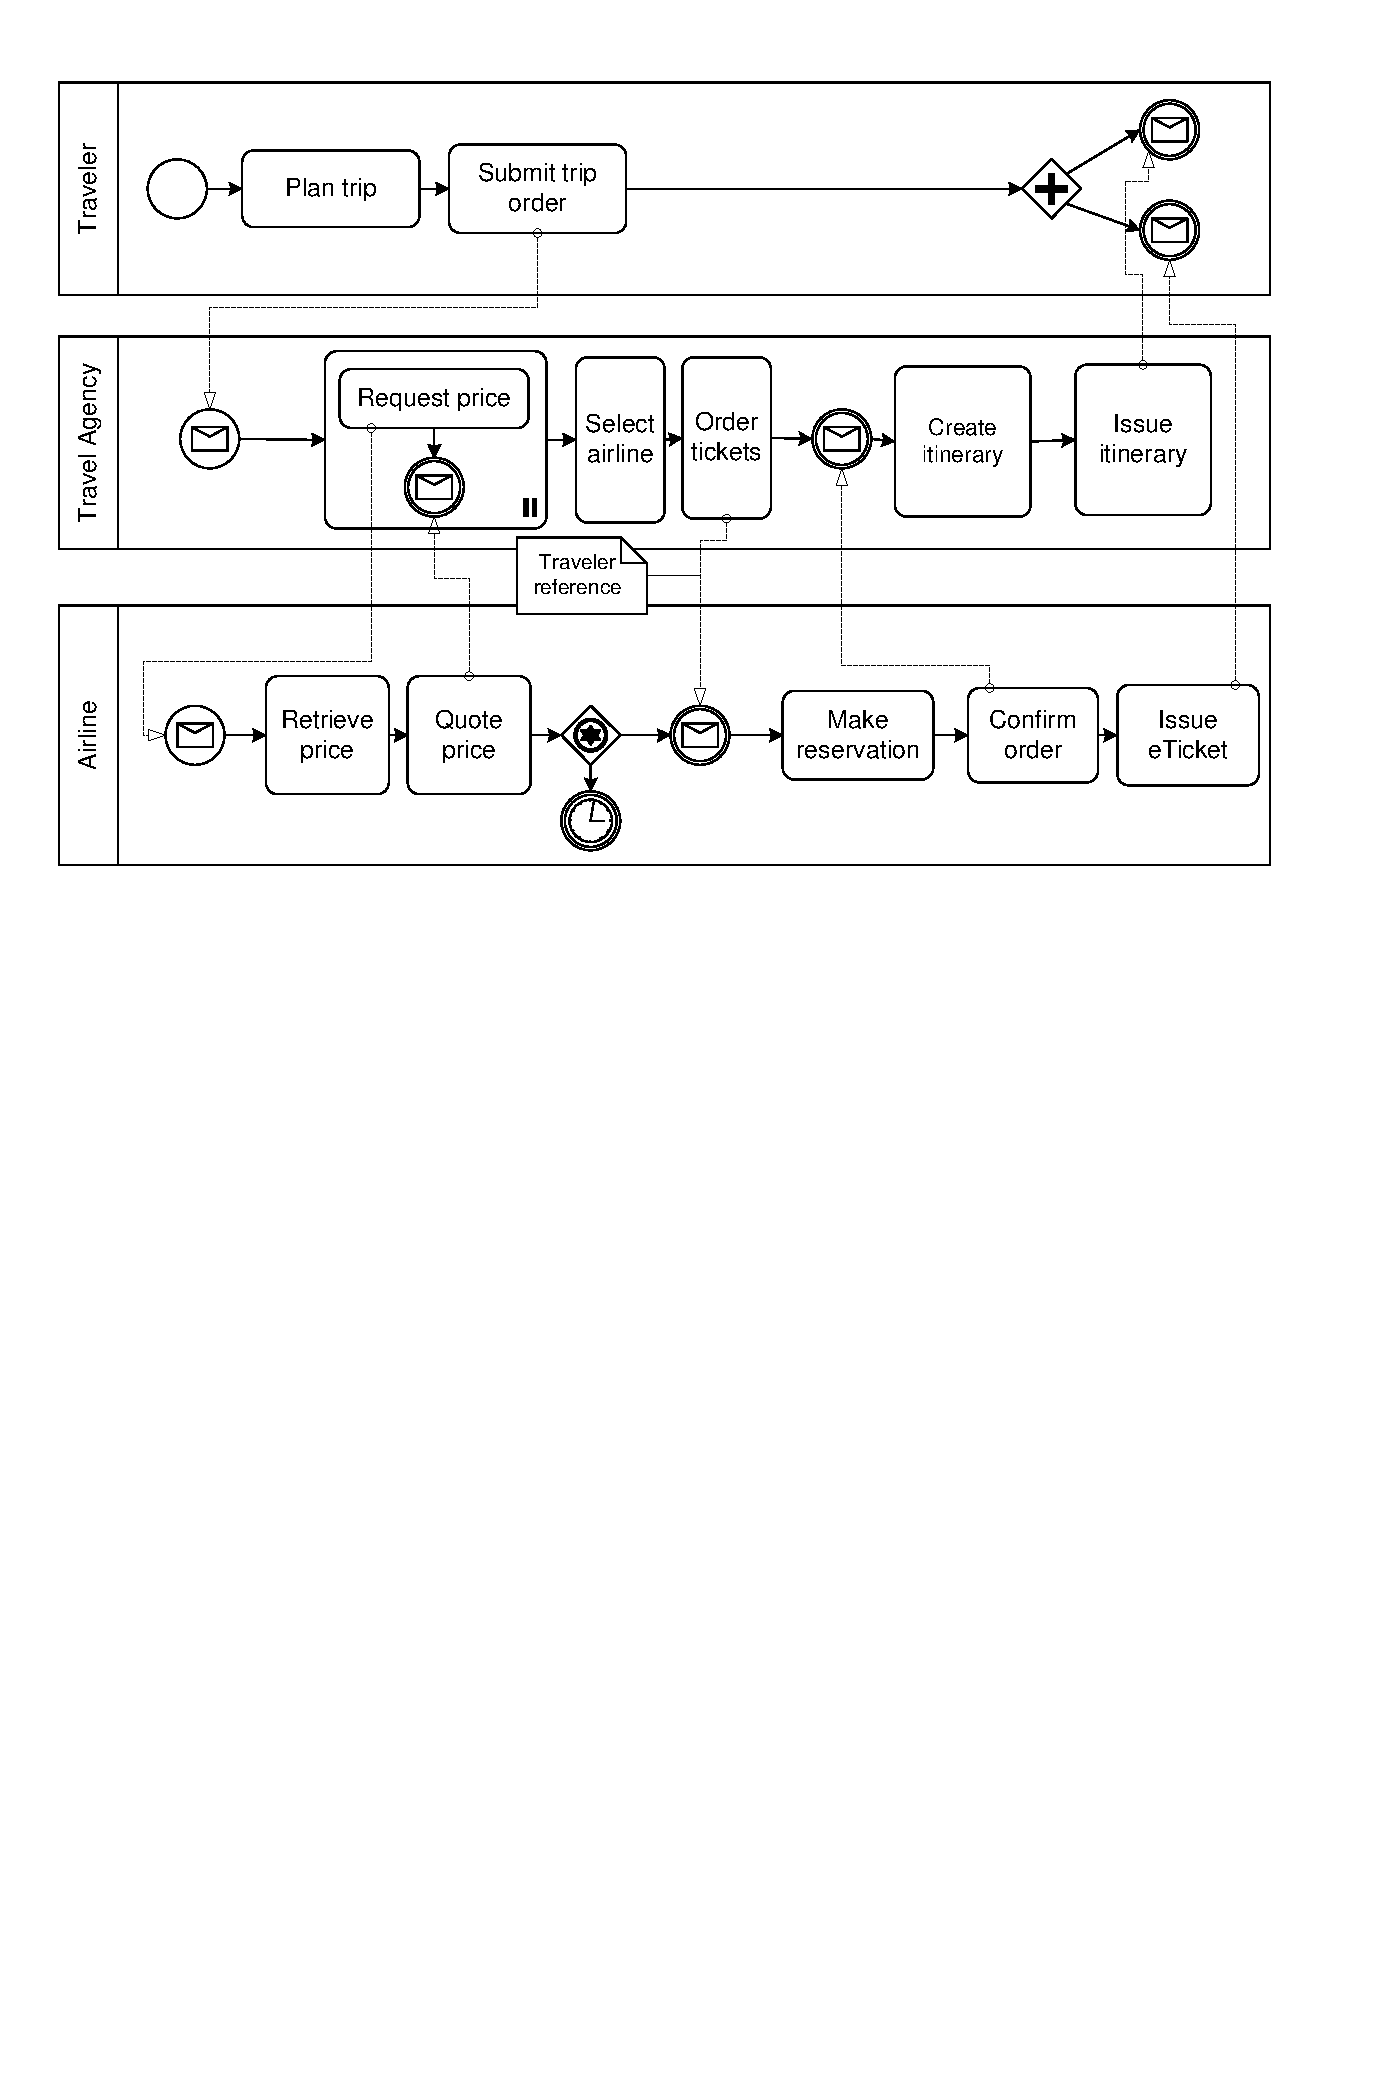
\includegraphics[width=.8\textwidth]{choreography.pdf}
  \caption[Example Choreography]{The example choreography. Now slightly smaller to demonstrate \texttt{\textbackslash textwidth}. And also the use of alternative captions for the list of images. However, the latter is only conditionally recommended, because who reads so much text under a picture? Or is it just a matter of style?}
  \label{fig:chor2}
\end{figure}


\begin{figure}
  \hfill
  \begin{subfigure}{.3\textwidth}
    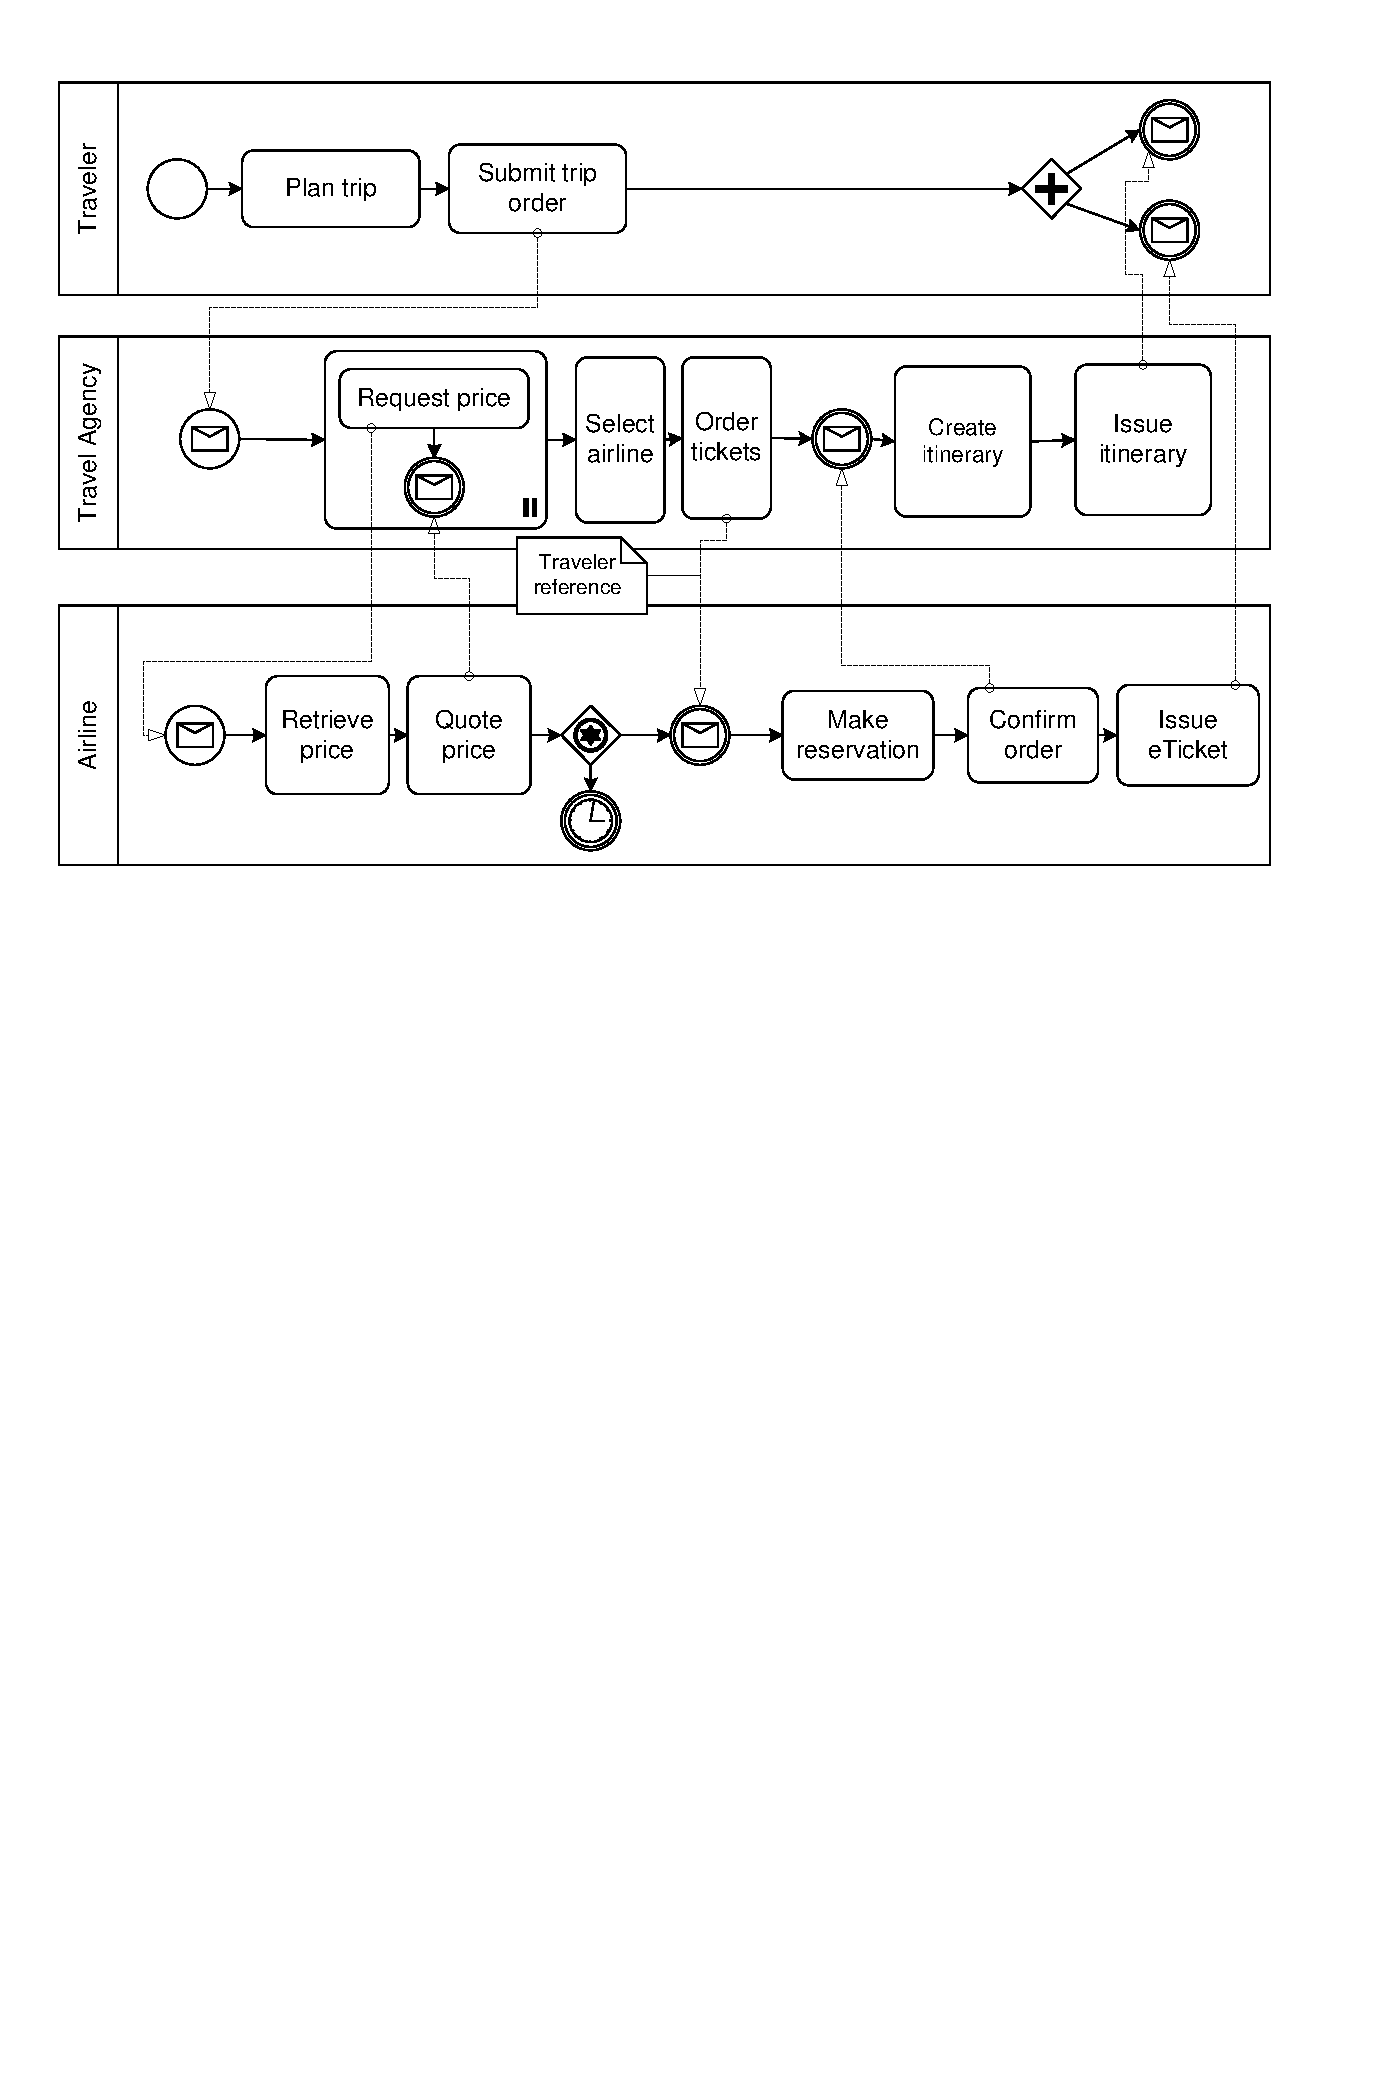
\includegraphics[width=\textwidth]{choreography.pdf}
    \caption{Choreography 1}
    \label{fig:subfigA}
  \end{subfigure}
  \hfill
  \begin{subfigure}{.3\textwidth}
    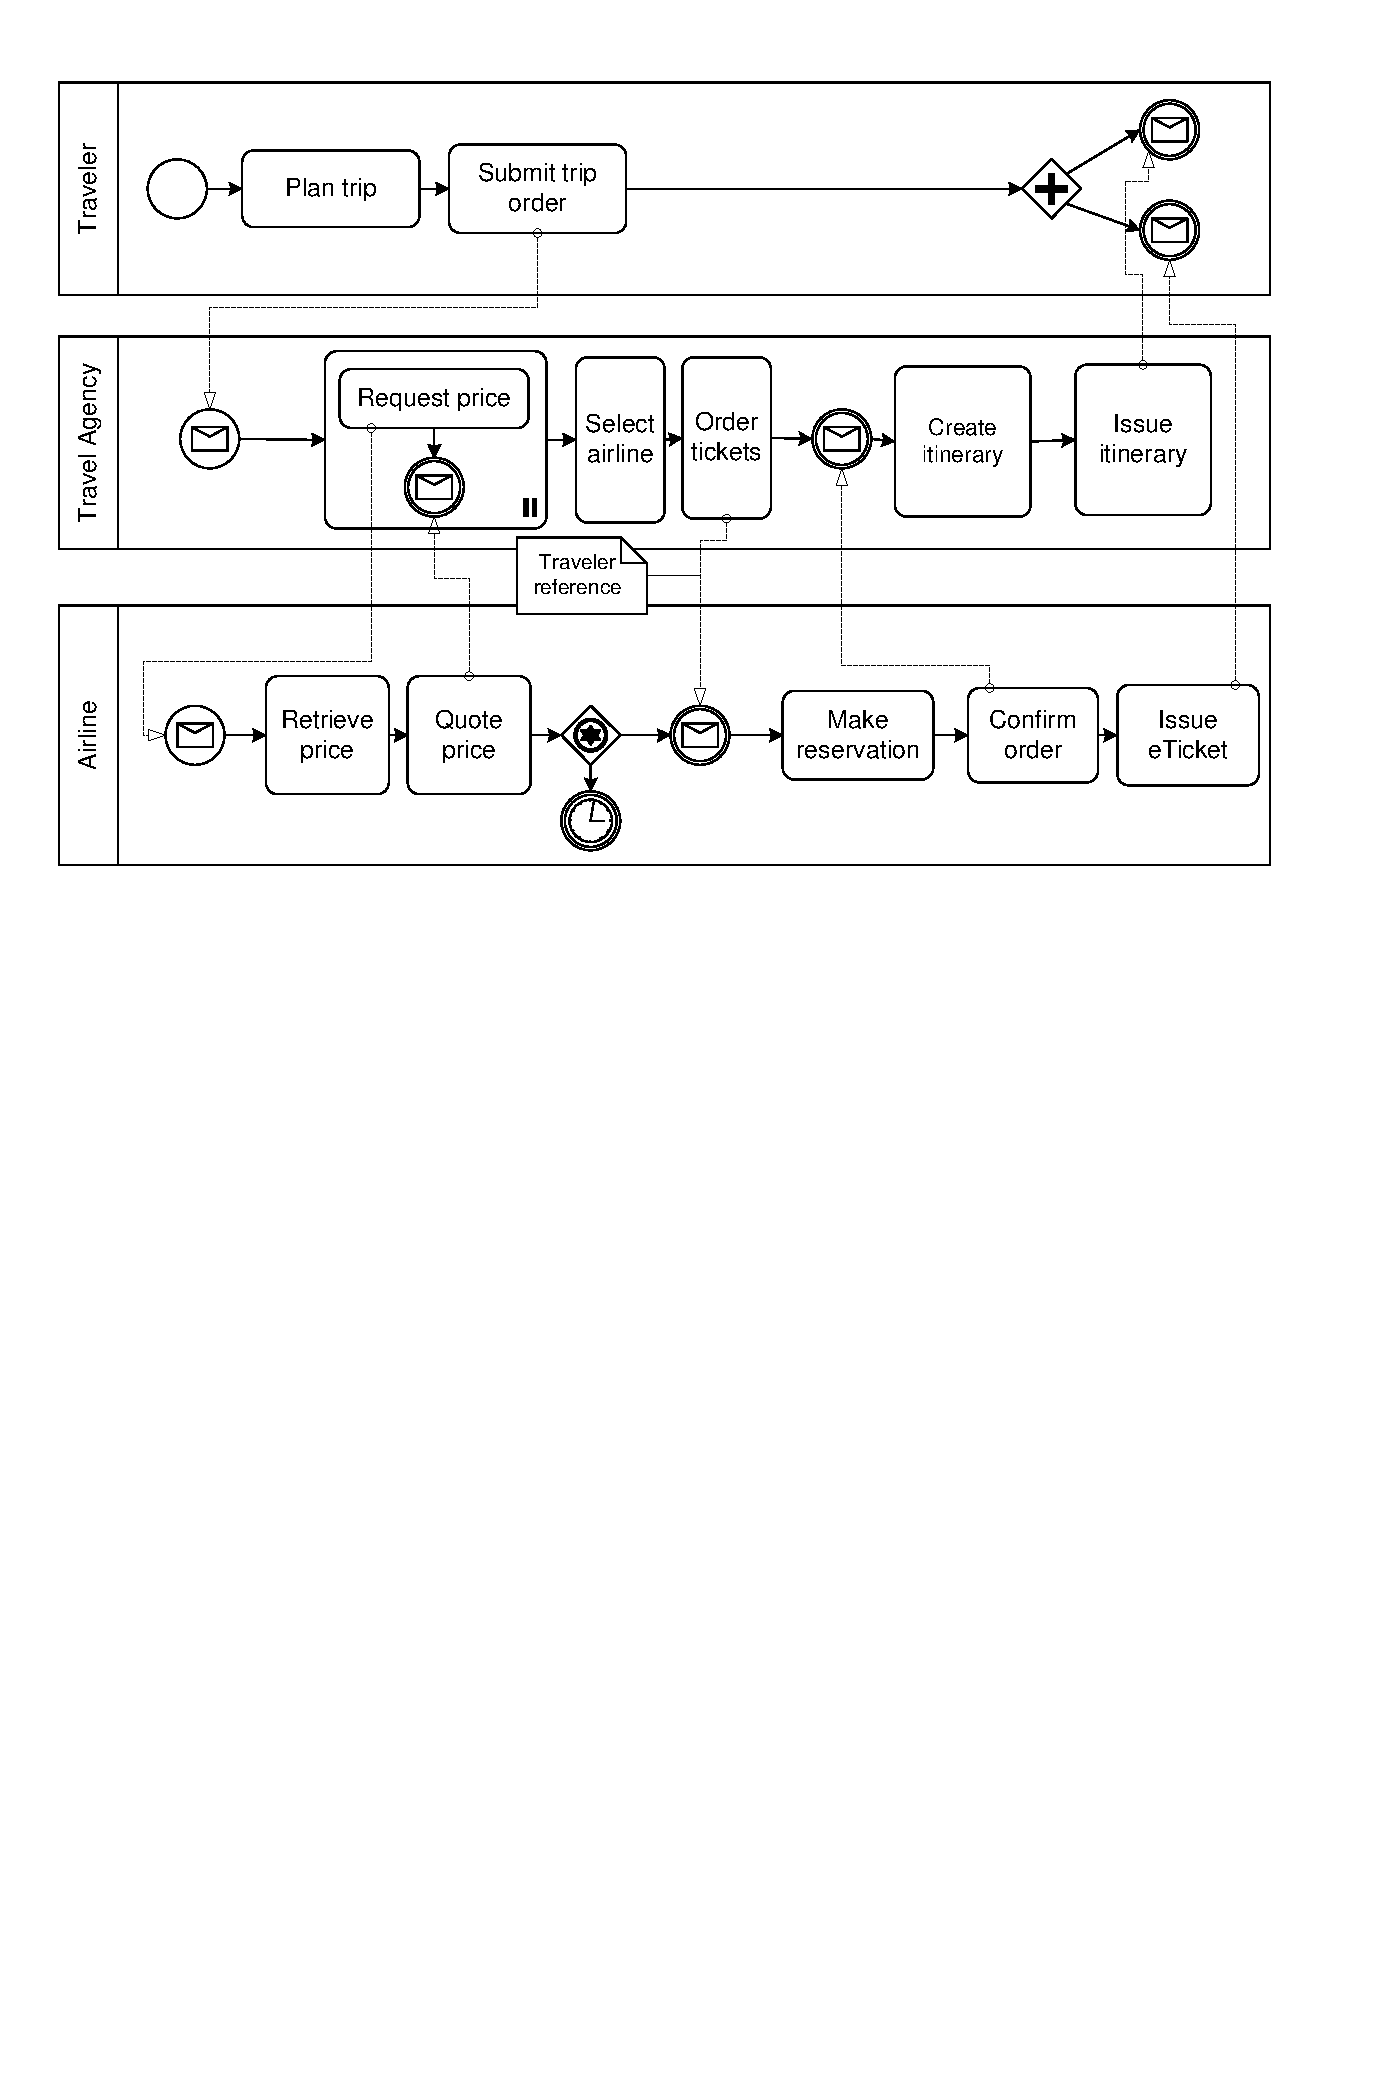
\includegraphics[width=\textwidth]{choreography.pdf}
    \caption{Choreography 2}
    \label{fig:subfigB}
  \end{subfigure}
  \hfill
  \begin{subfigure}{.3\textwidth}
    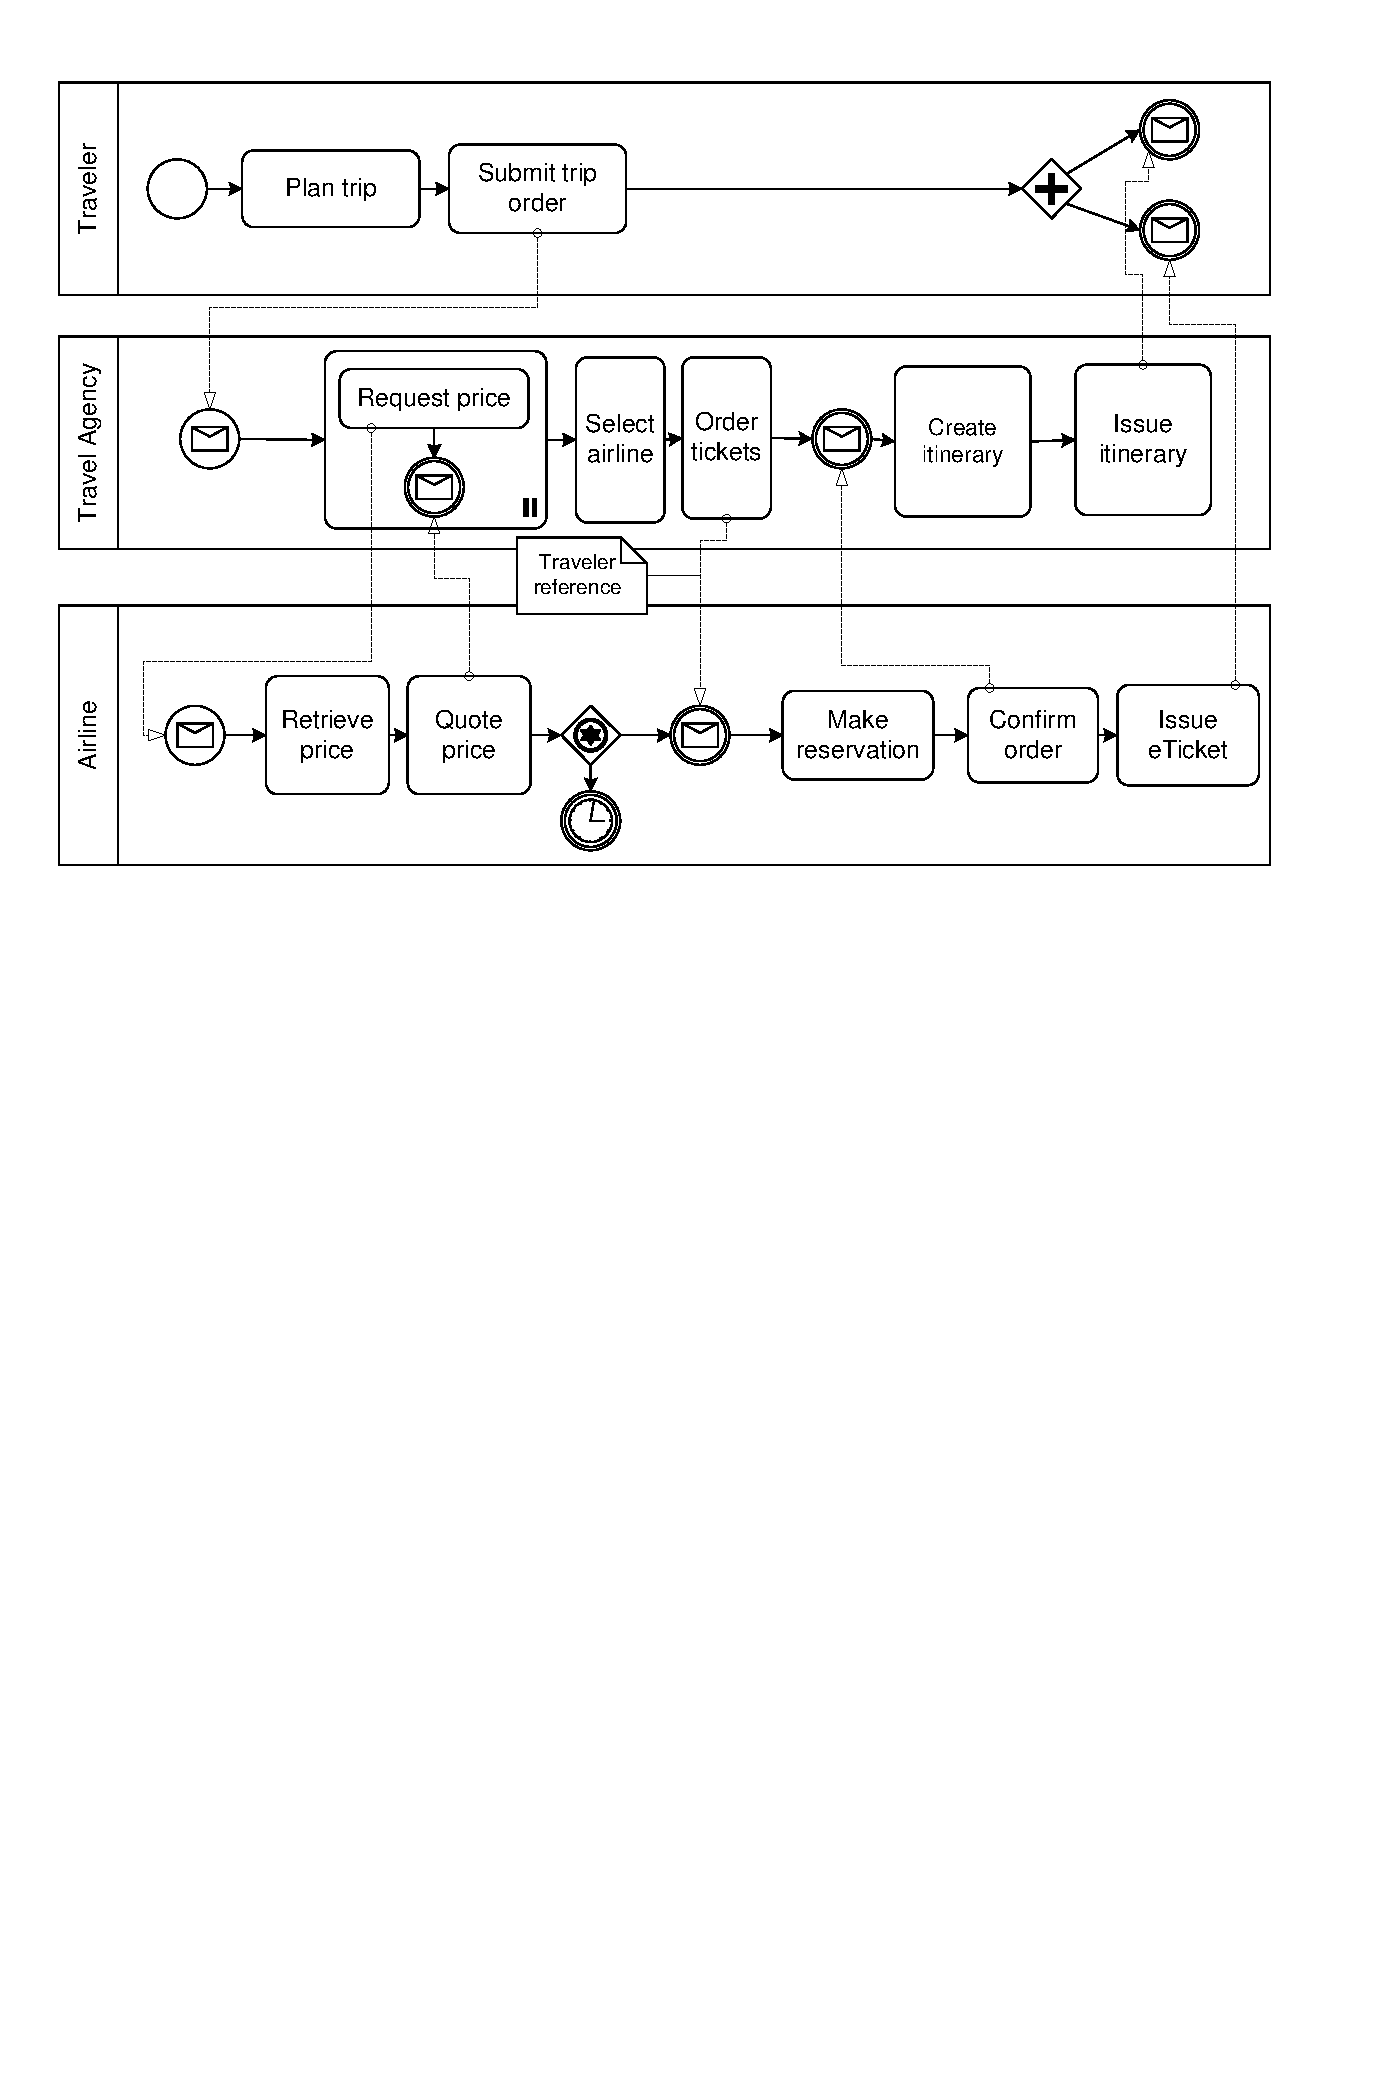
\includegraphics[width=.9\textwidth]{choreography.pdf}
    \caption{Choreography 3}
    \label{fig:subfigC}
  \end{subfigure}
  \caption{Example to place 3 illustrations next to each other. Further, it is possible to reference each separately.}
  \label{fig:subfig_example}
\end{figure}

\Cref{fig:subfig_example} shows the usage of the package subcaption.
It is indeed possible to reference to sub figures: \Cref{fig:subfigA}.

It is possible to convert SVGs to PDF directly during compilation.
This is described in the source code of latex-tipps.tex, but commented out.

\iffalse % <-- Take this away if inkscape is in the path
  The SVG in \cref{fig:directSVG} is directly included, while the text in the SVG in \cref{fig:latexSVG} is set using pdflatex.
  If you want to see the graphics, inkscape must be in PATH and in the text source \texttt{\textbackslash{}iffalse} and \text{\textbackslash{}iftrue} have to be commented out.

  \begin{figure}
    \centering
    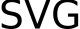
\includegraphics{svgexample.svg}
    \caption{SVG directly included}
    \label{fig:directSVG}
  \end{figure}

  \begin{figure}
    \centering
    \def\svgwidth{.4\textwidth}
    \includesvg{svgexample}
    \caption{Text in SVN set via \LaTeX{}}
    \label{fig:latexSVG}
  \end{figure}
\fi % <-- Take this away if inkscape is in the path



\section{More Illustrations}
\Cref{fig:AnhangsChor,fig:AnhangsChor2} show two choreographies, which should further explain the facts. The second figure is rotated 90 degrees to demonstrate the \texttt{pdflscape} package.

\begin{figure}
  \centering
  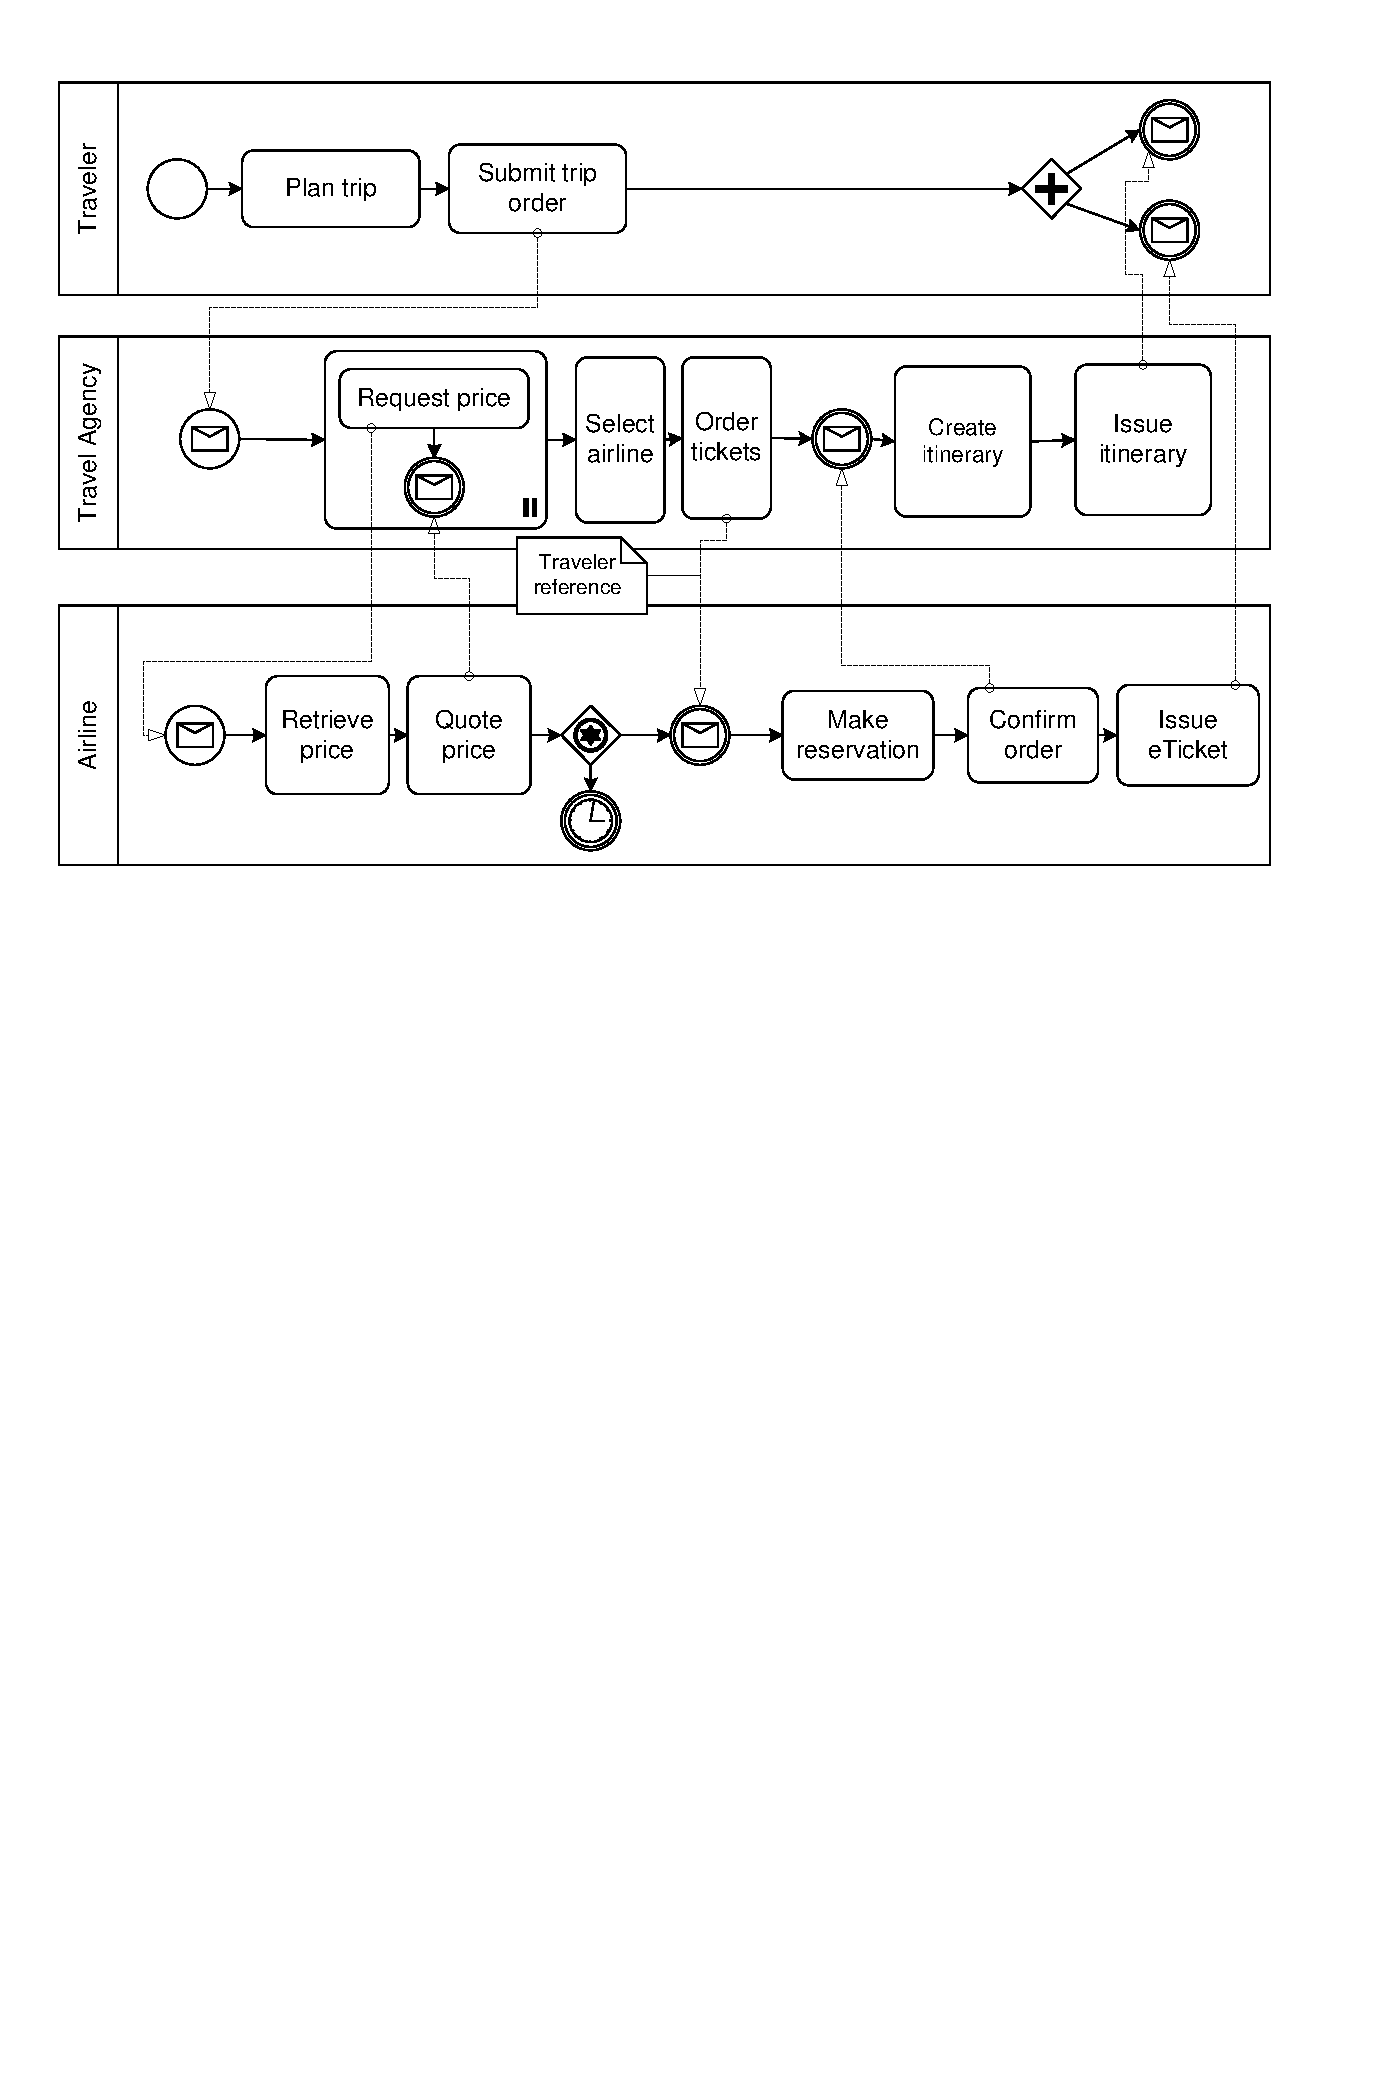
\includegraphics[width=\textwidth]{choreography.pdf}
  \caption{Example Choreography I}
  \label{fig:AnhangsChor}
\end{figure}

\begin{landscape}
  %sidewaysfigure
  \begin{figure}
    \centering
    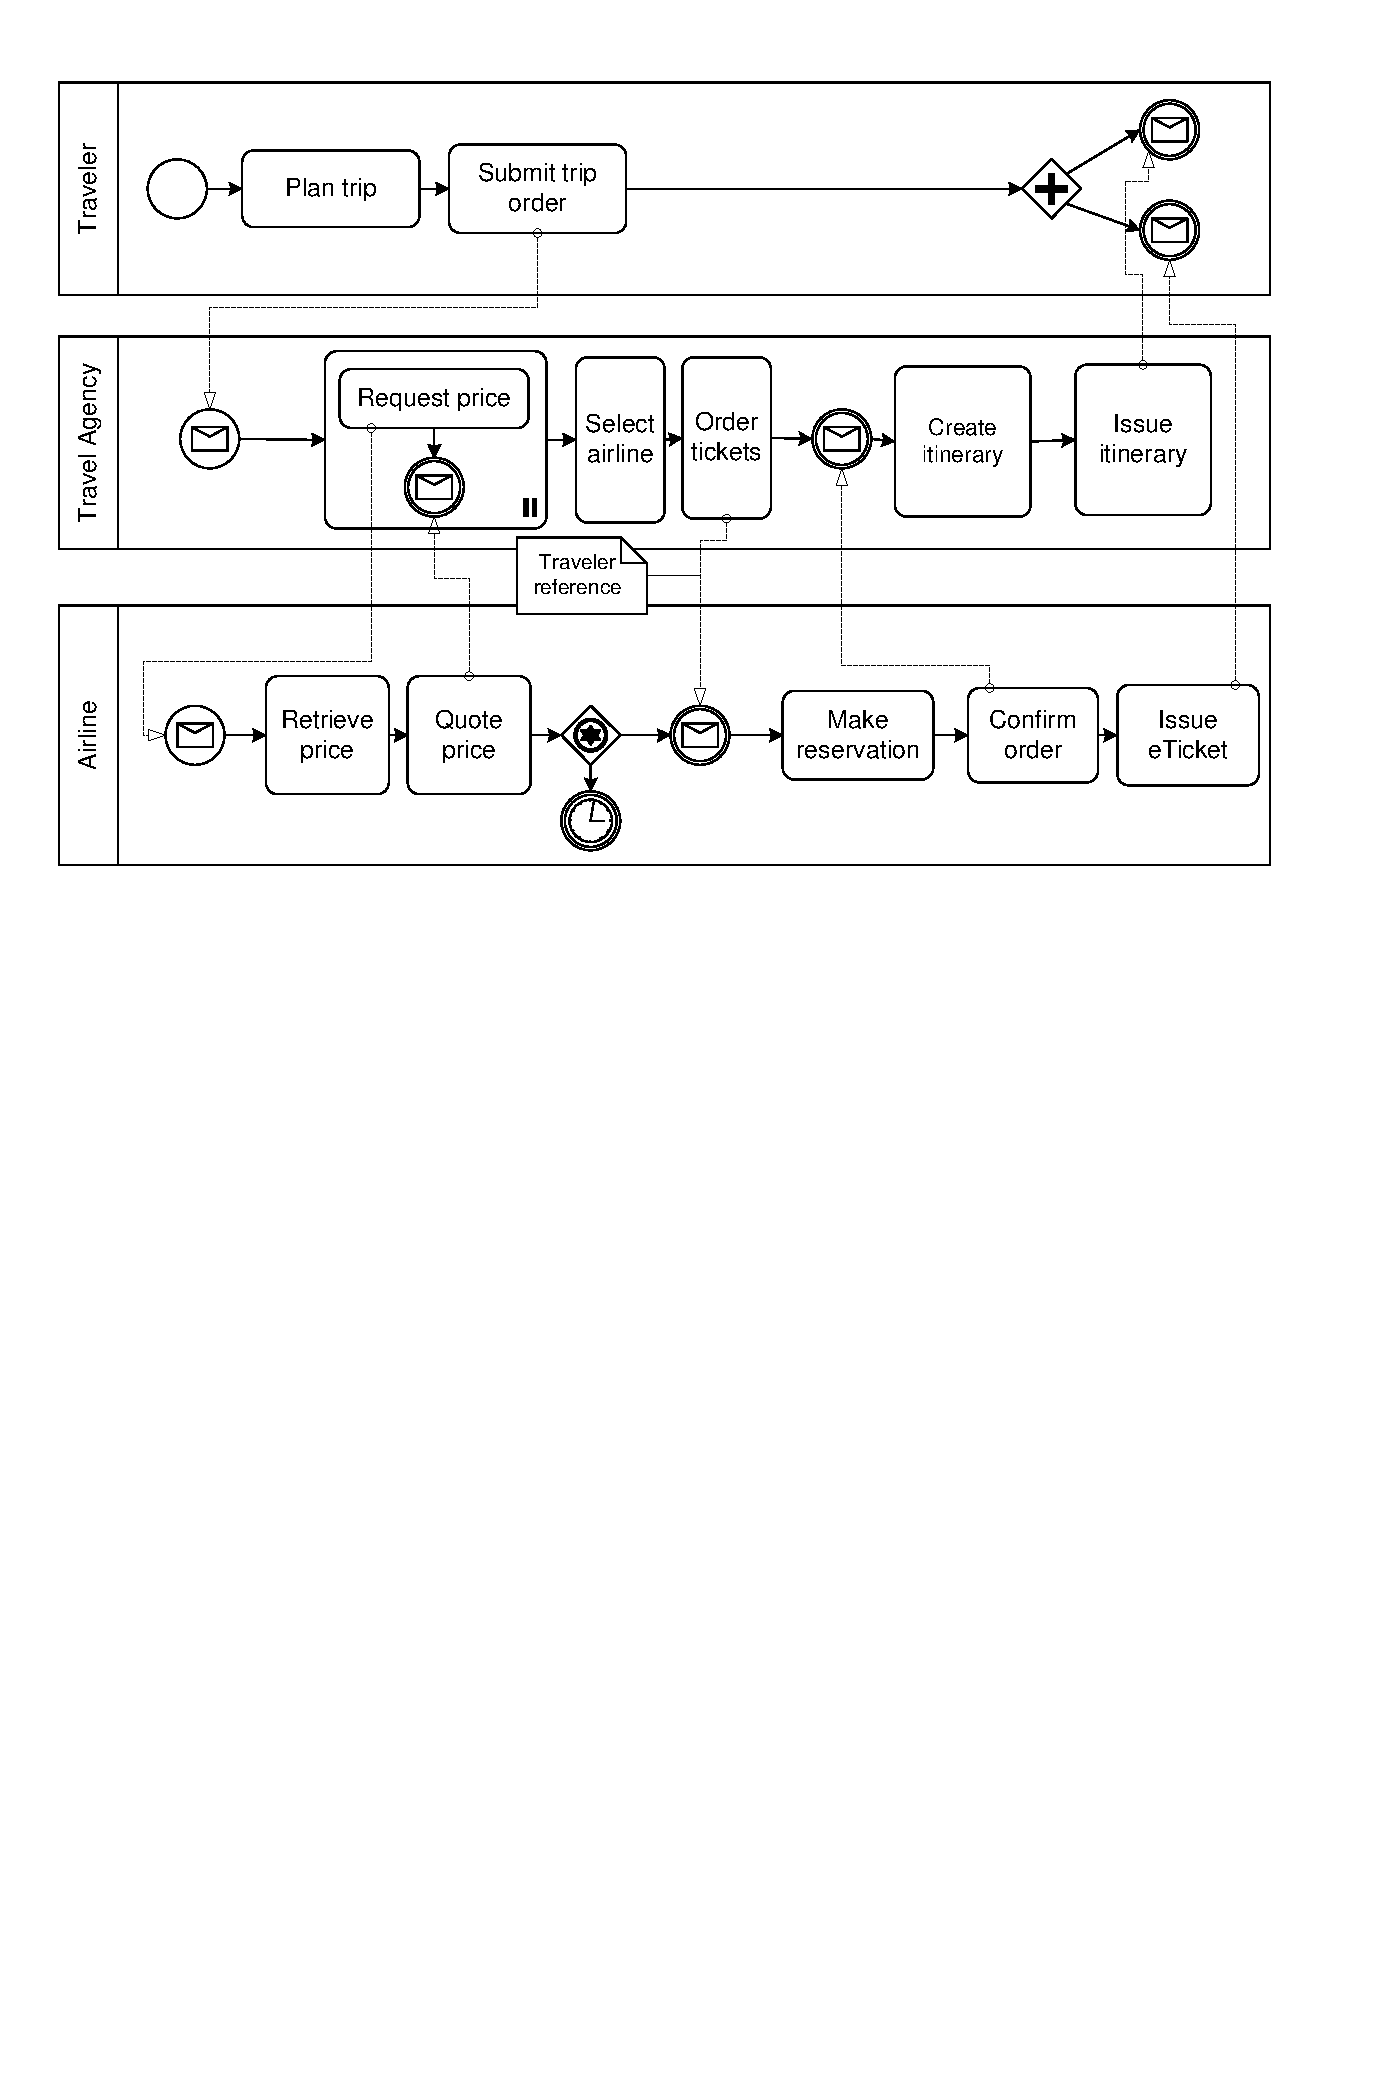
\includegraphics[width=\textwidth]{choreography.pdf}
    \caption{Example Choreography II}
    \label{fig:AnhangsChor2}
  \end{figure}
\end{landscape}


\IfFileExists{pgfplots.sty}{
  %%%%%%%%%%%%%%%%%%%%%%%%%%%%%%%%%%%%%%%%%%%%%%%%%%%%%%%%%%%%%%%%%%%%%%%%%%%%%%
  \section{Plots with pgfplots}
  %%%%%%%%%%%%%%%%%%%%%%%%%%%%%%%%%%%%%%%%%%%%%%%%%%%%%%%%%%%%%%%%%%%%%%%%%%%%%%
  The package pdfplots provides plotting of functions directly in \LaTeX~like with matlab or gnuplot. Some visual examples are available here\footnote{\url{http://texdoc.net/pkg/visualtikz}}.
  \begin{figure}[h]
    \centering
    \begin{tikzpicture}
      \begin{axis}[xlabel=$x$,
          ylabel=$\sin(x)$]
        \addplot {sin(deg(x))};  % Print sine function
      \end{axis}
    \end{tikzpicture}
    \caption{Plot of $\sin(x)$ direclty inside the figure environment with pgfplots.}
  \end{figure}

  \begin{figure}[h]
    \centering
    \begin{tikzpicture}
      \begin{axis}[xlabel=$x$,
          ylabel=$y$]
        \addplot table [x=a, y=c, col sep=comma] {data/data.csv};  % Read coordinates from csv file and plot them
      \end{axis}
    \end{tikzpicture}
    \caption{Coordinates $x$ and $y$ read from csv file and plotted pgfplots.}
  \end{figure}

}{}


%%%%%%%%%%%%%%%%%%%%%%%%%%%%%%%%%%%%%%%%%%%%%%%%%%%%%%%%%%%%%%%%%%%%%%%%%%%%%%
\section{Figures with tikz}
%%%%%%%%%%%%%%%%%%%%%%%%%%%%%%%%%%%%%%%%%%%%%%%%%%%%%%%%%%%%%%%%%%%%%%%%%%%%%%
The tikz is a package for creating graphics programmatically. With this package grids or other regular strucutres can be easliy generated.

\begin{figure}[ht]
  \centering
  \begin{tikzpicture}
    \draw(0,0) rectangle (4,4);
    \foreach \x in {0.5,1,1.5,2,2.5,3,3.5}
    \foreach \y in {0.5,1,1.5,2,2.5,3,3.5}
    \draw(\x,\y) circle (1pt);
  \end{tikzpicture}
  \caption{A regular grid genrated with easily with two for loops.}\label{fig:tikz_example}
\end{figure}


%%%%%%%%%%%%%%%%%%%%%%%%%%%%%%%%%%%%%%%%%%%%%%%%%%%%%%%%%%%%%%%%%%%%%%%%%%%%%%
\section{UML diagrams using tikz-uml}
%%%%%%%%%%%%%%%%%%%%%%%%%%%%%%%%%%%%%%%%%%%%%%%%%%%%%%%%%%%%%%%%%%%%%%%%%%%%%%

\Cref{fig:uml} presents a class diagram typeset using tikz-uml.

\begin{figure}
  \centering
  \begin{tikzpicture}
  \begin{umlpackage}{p}
  \begin{umlpackage}{sp1}
  \umlclass[template=T]{A}{
    n : uint \\ t : float
  }{}
  \umlclass[y=-3]{B}{
    d : double
  }{
    \umlvirt{setB(b : B) : void} \\ getB() : B}
  \end{umlpackage}
  \begin{umlpackage}[x=10,y=-6]{sp2}
  \umlinterface{C}{
    n : uint \\ s : string
  }{}
  \end{umlpackage}
  \umlclass[x=2,y=-10]{D}{
    n : uint
    }{}
  \end{umlpackage}

  \umlassoc[geometry=-|-, arg1=tata, mult1=*, pos1=0.3, arg2=toto, mult2=1, pos2=2.9, align2=left]{C}{B}
  \umlunicompo[geometry=-|, arg=titi, mult=*, pos=1.7, stereo=vector]{D}{C}
  \umlimport[geometry=|-, anchors=90 and 50, name=import]{sp2}{sp1}
  \umlaggreg[arg=tutu, mult=1, pos=0.8, angle1=30, angle2=60, loopsize=2cm]{D}{D}
  \umlinherit[geometry=-|]{D}{B}
  \umlnote[x=2.5,y=-6, width=3cm]{B}{A note with respect to class B}
  \umlnote[x=7.5,y=-2]{import-2}{A anotation}
  \end{tikzpicture}
  \caption{Class diagram generated with tikz-uml. Example adapted from Nicolas Kielbasiewicz.}
  \label{fig:uml}
\end{figure}

\section{UML diagrams using PlantUML}

In case \lualatex{} is used and PlantUML is installed, UML diagrams can be defined using PlantUML.

% Only works if "--shell-escape" is activated. Please activate only if you are sure, your compilation settings are correct
%\IfFileExists{plantuml.sty}{\input{latexhints-english-plantuml}}{}


%%%%%%%%%%%%%%%%%%%%%%%%%%%%%%%%%%%%%%%%%%%%%%%%%%%%%%%%%%%%%%%%%%%%%%%%%%%%%%
\section{Linguistic Forests}
%%%%%%%%%%%%%%%%%%%%%%%%%%%%%%%%%%%%%%%%%%%%%%%%%%%%%%%%%%%%%%%%%%%%%%%%%%%%%%

\begin{filecontents*}[overwrite]{\democodefile}
\begin{forest}
  [VP
    [DP]
    [V’
      [V]
      [DP]
    ]
  ]
\end{forest}
\end{filecontents*}
\PrintDemo{style=parallel}


%%%%%%%%%%%%%%%%%%%%%%%%%%%%%%%%%%%%%%%%%%%%%%%%%%%%%%%%%%%%%%%%%%%%%%%%%%%%%%
\section{Tables}
%%%%%%%%%%%%%%%%%%%%%%%%%%%%%%%%%%%%%%%%%%%%%%%%%%%%%%%%%%%%%%%%%%%%%%%%%%%%%%
\cref{tab:Ergebnisse} shows results and \cref{tab:Werte} shows how numerical data can be represented in a table.
\begin{table}
  \centering
  \begin{tabular}{ccc}
    \toprule
    \multicolumn{2}{c}{\textbf{summed}} & \textbf{Title}                                                          \\ \midrule
    Table                                      & as                                                           & in      \\
    \url{tabsatz.pdf}                            & recommended                                                     & gesetzt \\

    \multirow{2}{*}{Example}                    & \multicolumn{2}{c}{a nice example}                                \\
                                                 & \multicolumn{2}{c}{for using \qq{multirow}}           \\
    \bottomrule
  \end{tabular}
  \caption[Example Table]{Exampe Table -- see \url{http://www.ctan.org/tex-archive/info/german/tabsatz/}}
  \label{tab:Ergebnisse}
\end{table}

\begin{table}
  \centering
  \begin{tabular}{l *{8}{d{3.2}}}
    \toprule

                         & \multicolumn{2}{c}{\textbf{Parameter 1}} & \multicolumn{2}{c}{\textbf{Parameter 2}} & \multicolumn{2}{c}{\textbf{Parameter 3}} & \multicolumn{2}{c}{\textbf{Parameter 4}}                                                                                                                                       \\
    \cmidrule(r){2-3}\cmidrule(lr){4-5}\cmidrule(lr){6-7}\cmidrule(l){8-9}

    \textbf{Bedingungen} & \multicolumn{1}{c}{\textbf{M}}           & \multicolumn{1}{c}{\textbf{SD}}          & \multicolumn{1}{c}{\textbf{M}}           & \multicolumn{1}{c}{\textbf{SD}}          & \multicolumn{1}{c}{\textbf{M}} & \multicolumn{1}{c}{\textbf{SD}} & \multicolumn{1}{c}{\textbf{M}} & \multicolumn{1}{c}{\textbf{SD}} \\
    \midrule

    W                    & 1.1                                      & 5.55                                     & 6.66                                     & .01                                      &                                &                                 &                                &                                 \\
    X                    & 22.22                                    & 0.0                                      & 77.5                                     & .1                                       &                                &                                 &                                &                                 \\
    Y                    & 333.3                                    & .1                                       & 11.11                                    & .05                                      &                                &                                 &                                &                                 \\
    Z                    & 4444.44                                  & 77.77                                    & 14.06                                    & .3                                       &                                &                                 &                                &                                 \\
    \bottomrule
  \end{tabular}

  \caption{Example table for 4 constraints (W-Z), each having 4 parameters with (M und SD). Note: use always the same number of decimal places.}
  \label{tab:Werte}
\end{table}

\IfFileExists{pgfplotstable.sty}{

\subsection{Tables with pgfplots}
With the pgfplotstable package tables can be directly generated from a csv file.

\begin{table}[h]
\centering
\pgfplotstabletypeset[
col sep = comma,
every head row/.style={before row=\toprule,after row=\midrule},
every last row/.style={after row=\bottomrule},
display columns/0/.style={string type,column name={}}
]
{data/data.csv}
\caption{Table direclty generated from the values of a csf file.}
\end{table}
}{}


\section{Tables spanning multiple pages}


\begin{longtable}{|l|l|l|}
\caption{A sample long table.} \label{tab:long} \\

\hline \multicolumn{1}{|c|}{\textbf{First column}} & \multicolumn{1}{c|}{\textbf{Second column}} & \multicolumn{1}{c|}{\textbf{Third column}} \\ \hline
\endfirsthead

\multicolumn{3}{c}%
{{\bfseries \tablename\ \thetable{} -- continued from previous page}} \\
\hline \multicolumn{1}{|c|}{\textbf{First column}} & \multicolumn{1}{c|}{\textbf{Second column}} & \multicolumn{1}{c|}{\textbf{Third column}} \\ \hline
\endhead

\hline \multicolumn{3}{|r|}{{Continued on next page}} \\ \hline
\endfoot

\hline \hline
\endlastfoot

A & BC & D \\
A & BC & D \\
A & BC & D \\
A & BC & D \\
A & BC & D \\
A & BC & D \\
A & BC & D \\
A & BC & D \\
A & BC & D \\
A & BC & D \\
A & BC & D \\
A & BC & D \\
A & BC & D \\
A & BC & D \\
A & BC & D \\
A & BC & D \\
A & BC & D \\
A & BC & D \\
A & BC & D \\
A & BC & D \\
A & BC & D \\
A & BC & D \\
A & BC & D \\
A & BC & D \\
A & BC & D \\
A & BC & D \\
A & BC & D \\
A & BC & D \\
A & BC & D \\
A & BC & D \\
A & BC & D \\
A & BC & D \\
A & BC & D \\
A & BC & D \\
A & BC & D \\
A & BC & D \\
A & BC & D \\
A & BC & D \\
A & BC & D \\
A & BC & D \\
A & BC & D \\
A & BC & D \\
A & BC & D \\
A & BC & D \\
A & BC & D \\
A & BC & D \\
A & BC & D \\
A & BC & D \\
A & BC & D \\
A & BC & D \\
A & BC & D \\
A & BC & D \\
A & BC & D \\
A & BC & D \\
A & BC & D \\
A & BC & D \\
A & BC & D \\
A & BC & D \\
A & BC & D \\
A & BC & D \\
A & BC & D \\
A & BC & D \\
A & BC & D \\
A & BC & D \\
A & BC & D \\
A & BC & D \\
A & BC & D \\
A & BC & D \\
A & BC & D \\
A & BC & D \\
A & BC & D \\
A & BC & D \\
A & BC & D \\
A & BC & D \\
A & BC & D \\
A & BC & D \\
A & BC & D \\
A & BC & D \\
A & BC & D \\
A & BC & D \\
\end{longtable}


%%%%%%%%%%%%%%%%%%%%%%%%%%%%%%%%%%%%%%%%%%%%%%%%%%%%%%%%%%%%%%%%%%%%%%%%%%%%%%
\section{Abbreviations}
%%%%%%%%%%%%%%%%%%%%%%%%%%%%%%%%%%%%%%%%%%%%%%%%%%%%%%%%%%%%%%%%%%%%%%%%%%%%%%
At the first pass the \gls{fr} was 5.
At the second pass was \gls{fr} 3.
The plural form can be seen here: \glspl{er}.
To demonstrate what the list of abbreviations looks like for longer description texts, \glspl{rdbms} must be mentioned here.

With \verb+\gls{...}+ you can enter abbreviations, the first time you call it, the long form is used.
When reusing \verb+\gls{..}+ the short form is automatically displayed.
The abbreviation is also automatically inserted in the abbreviation list.
With \verb+\glspl{...}+ the plural form is used.
If you want the short form to appear directly at the first use, you can use \verb+\glsunset{..}+ to mark an abbreviation as already used.
The opposite is achieved with \verb+\glsreset{..}+.

Abbreviations are defined in \verb+\content\ausarbeitung.tex+ by means of \verb+\newacronym{...}{...}{...}+.

More information at: \url{http://tug.ctan.org/macros/latex/contrib/glossaries/glossariesbegin.pdf}
%%%%%%%%%%%%%%%%%%%%%%%%%%%%%%%%%%%%%%%%%%%%%%%%%%%%%%%%%%%%%%%%%%%%%%%%%%%%%%
\section{References}
%%%%%%%%%%%%%%%%%%%%%%%%%%%%%%%%%%%%%%%%%%%%%%%%%%%%%%%%%%%%%%%%%%%%%%%%%%%%%%
For distant sections \qq{varioref} is recommended:
\qq{See \vref{sec:mf}}.
The command \texttt{\textbackslash{}vref} works similar to \texttt{\textbackslash{}cref} the difference beeing that a reference to the page is additionally added.
\texttt{vref}: \qq{\vref{sec:firstsectioninlatexhints}}, \texttt{cref}: \qq{\cref{sec:firstsectioninlatexhints}}, \texttt{ref}: \qq{\ref{sec:firstsectioninlatexhints}}.

If \qq{varioref} causes difficulties, then \qq{cref} can be used instead.
This also creates the word \qq{section} automatically: \cref{sec:mf}.
This is also possible for illustrations etc.
In English please use \verb1\Cref{...}1 (with large \qq{C} at the beginning).

%With MiKTeX installation from 2012-01-16 no longer necessary.
%If a section becomes longer than one page and you want to refer to a specific place in the section with \texttt{\textbackslash{}vref}, then you should use \texttt{\textbackslash{}phantomsection} then using \texttt{vref} will also display the correct page number.

%%The link location will be placed on the line below.
%%Tipp von http://en.wikibooks.org/wiki/LaTeX/Labels_and_Cross-referencing#The_hyperref_package_and_.5Cphantomsection
%\phantomsection
%\label{alabel}
%View the example for \texttt{\textbackslash{}phantomsection} in the \LaTeX{} source code.

%Here is the example: See Section \vref{hack1} and Section \vref{hack2}.
%%%%%%%%%%%%%%%%%%%%%%%%%%%%%%%%%%%%%%%%%%%%%%%%%%%%%%%%%%%%%%%%%%%%%%%%%%%%%%
\section{Definitions}
%%%%%%%%%%%%%%%%%%%%%%%%%%%%%%%%%%%%%%%%%%%%%%%%%%%%%%%%%%%%%%%%%%%%%%%%%%%%%%
\begin{definition}[Title]
  \label{def:def1}
  Definition Text
\end{definition}

\Cref{def:def1} shows \ldots

%%%%%%%%%%%%%%%%%%%%%%%%%%%%%%%%%%%%%%%%%%%%%%%%%%%%%%%%%%%%%%%%%%%%%%%%%%%%%%
\section{Footnotes}
%%%%%%%%%%%%%%%%%%%%%%%%%%%%%%%%%%%%%%%%%%%%%%%%%%%%%%%%%%%%%%%%%%%%%%%%%%%%%%
Footnotes are provided by the command \verb+\footnote{...}+\footnote{\label{fussnote}Example footnote.}. Citing footnotes is possible by provinding a label\verb+\footnote{\label{...}...}+ and cite the footnote with \verb+\cref{...}+ in the text\cref{fussnote}.
%%%%%%%%%%%%%%%%%%%%%%%%%%%%%%%%%%%%%%%%%%%%%%%%%%%%%%%%%%%%%%%%%%%%%%%%%%%%%%

%%%%%%%%%%%%%%%%%%%%%%%%%%%%%%%%%%%%%%%%%%%%%%%%%%%%%%%%%%%%%%%%%%%%%%%%%%%%%%
\section{Various Things}
%%%%%%%%%%%%%%%%%%%%%%%%%%%%%%%%%%%%%%%%%%%%%%%%%%%%%%%%%%%%%%%%%%%%%%%%%%%%%%
\label{sec:diff}
\ifdeutsch
  Numbers (123\,654\,789) are nicely set.
  Either in a line or as non-lining figure.
  The latter is reached by parameter \texttt{osf} at package \texttt{libertine} or.\ \texttt{mathpazo} in \text{fonts.tex}.
\fi

\begin{filecontents*}[overwrite]{\democodefile}
\begin{compactenum}[I.]
  \item You can also keep the numbering compact thanks to paralist
  \item and switch to a different numbering
\end{compactenum}
\end{filecontents*}
\PrintDemo{style=parallel}

The words \qq{workflow} and \qq{dwarflike} can be copied from the PDF and pasted to a text file.

\begin{filecontents*}[overwrite]{\democodefile}
In case \LuaLaTeX{} is used as compiler, there is no ligature at \qq{f\/l} in the word \qq{dwarflike} (in contrast to \qq{fl} at \qq{workflow}).
In other words: \qq{dwarflike} and \qq{dwarf\/like} look the same in the PDF.
In case they do not, there is an issue with Lua\LaTeX{} and the selnolig package.
\end{filecontents*}
\PrintDemo{style=parallel}
% Meta comment: The precise form of the optimal ligation suppression command may vary depending on the character pairs involved - see https://tex.stackexchange.com/q/28437/9075


%%%%%%%%%%%%%%%%%%%%%%%%%%%%%%%%%%%%%%%%%%%%%%%%%%%%%%%%%%%%%%%%%%%%%%%%%%%%%%
\section{Closing remarks}
%%%%%%%%%%%%%%%%%%%%%%%%%%%%%%%%%%%%%%%%%%%%%%%%%%%%%%%%%%%%%%%%%%%%%%%%%%%%%%
Please feel free to provide enhancements for this template and create a new ticket on GitHub (\url{https://github.com/latextemplates/uni-stuttgart-computer-science-template/issues}).


\pagestyle{empty}
\renewcommand*{\chapterpagestyle}{empty}
\Versicherung
\end{document}
